%---------------------------------------------------------------------------------------
%	PACKAGES AND THEMES
%---------------------------------------------------------------------------------------
\documentclass[aspectratio=169,xcolor=dvipsnames]{beamer} % handout

\newcommand{\backupbegin}{
   \newcounter{finalframe}
   \setcounter{finalframe}{\value{framenumber}}
}
\newcommand{\backupend}{
   \setcounter{framenumber}{\value{finalframe}}
}

\newcommand\T{\rule{0pt}{2.6ex}}       % Top strut
\newcommand\B{\rule[-1.2ex]{0pt}{0pt}} % Bottom strut
\usepackage{array}
\newcolumntype{P}[1]{>{\centering\arraybackslash}p{#1}}
\newcolumntype{M}[1]{>{\centering\arraybackslash}m{#1}}
\usetheme{SimplePlus}
\usepackage{xcolor}
\usepackage{hyperref}
\usepackage{graphicx} % Allows including images/logos
\usepackage{booktabs} % Allows the use of \toprule, \midrule and \bottomrule in tables
\usepackage{comment}
\usepackage{tikz}
\usepackage{mhchem}
\usepackage{setspace}
\usepackage{array}
\newcolumntype{L}[1]{>{\raggedright\let\newline\\\arraybackslash\hspace{0pt}}m{#1}}
\newcolumntype{C}[1]{>{\centering\let\newline\\\arraybackslash\hspace{0pt}}m{#1}}
\newcolumntype{R}[1]{>{\raggedleft\let\newline\\\arraybackslash\hspace{0pt}}m{#1}}
\usepackage{setspace}
\usepackage{amsmath}
\usepackage{siunitx}
\sisetup{detect-all}
\usepackage{pifont}
\newcommand{\xmark}{\ding{55}}
\usepackage{svg}
\usepackage[absolute,overlay]{textpos}
\usepackage{bm}
\newcommand{\greencheck}{{\color{ForestGreen}\checkmark}}
\newcommand{\redcross}{{\color{Red}\xmark}}

% all pages logos
\logo{
    \begin{picture}(0,0)
        \put(0,0){\makebox(-60,235)[rt]{\includesvg[width=1cm]{images/logos/unibg_logo_single.svg}}}
         \put(0,0){\makebox(-25,235)[rt]{
\includegraphics[width=0.7cm]{images/logos/gaps.png}}}
    \end{picture}
}

\setbeamercovered{transparent}
\setbeamertemplate{footline}[frame number]{}


%-------------------------------------------------------------------------------
%	PDF METADATA
%-------------------------------------------------------------------------------

\hypersetup{
    pdfauthor={Luca Ghislotti},
    pdftitle={Characterisation of the readout electronics of the Si(Li) tracker for the first flight of the GAPS experiment},
    pdfsubject={This thesis work describes the characterisation work that has been carried out on the flight items of the lithium-drifted silicon tracker of the GAPS experiment and includes an in-depth description of the validation techniques used for all detector components and the results obtained during the testing process.},
    pdfkeywords={GAPS, Dark Matter, ASIC, Microelectronics},
    pdfproducer={Overleaf},
    pdfcreator={PdfTeX}
}


%---------------------------------------------------------------------------------------
%	TITLE PAGE
%---------------------------------------------------------------------------------------

\title[]{\large{Characterisation of the readout electronics of the Si(Li) tracker\\ for the first flight of the GAPS experiment}} % The short title appears at the bottom of every slide, the full title is only on the title page

\author[Luca Ghislotti] {Luca Ghislotti\\Master Thesis Defence\\ \vspace{0.3cm}\small September $30^{\text{th}}$, 2022}

\institute[UniBG]{
    \\Supervisor: prof. Massimo Manghisoni \\
    Co-Supervisors: Ph.D. Elisa Riceputi, M.Sc. Paolo Lazzaroni
}

\date{Computer Engineering\\Academic Year 2021/2022} % Date

% title page logos
\titlegraphic { 
    \begin{picture}(0,0)
        % VERSION WITH UNIBG AND GAPS LOGOS
        \put(25,164){\makebox(0,0)[rt]{
\includegraphics[width=4cm]{images/logos/unibg-logo.png}}}
        \put(90,170){\makebox(0,0)[rt]{
\includegraphics[width=1.4cm]{images/logos/gaps.png}}}
    \end{picture}
}

\begin{document}


%---------------------------------------------------------------------------------------
%	TITLE PAGE
%---------------------------------------------------------------------------------------

\frame[plain]{
    \vspace{-0.5cm}
    \titlepage
}


%---------------------------------------------------------------------------------------
%	General AntiParticle Spectrometer (GAPS)
%---------------------------------------------------------------------------------------

\begin{frame}{General AntiParticle Spectrometer (GAPS)}
\fontsize{9pt}{1}\selectfont
   \begin{columns}
   \vspace{0.05cm}
    \column{0.58\textwidth}
        \vskip0.2cm
        \pause
        GAPS is an \textbf{Antarctic balloon experiment} designed to detect low-energy cosmic antinuclei as an indirect signature of \textbf{Dark Matter}\\\pause
        \vspace{0.3cm}
        \textbf{\large \textcolor{ForestGreen}{The instrument}}\\
        \vspace{0.25cm}
        \textbf{\textcolor{Red}{Time-of-Flight System (TOF)}}
        \begin{itemize}
            \item 220 plastic scintillator paddles with Si-PM readout
        \end{itemize}\pause
        \vspace{0.15cm}
        \textbf{\textcolor{Red}{Si(Li) Tracker}}
        \begin{itemize}
            \item About 1000 lithium-drifted silicon (Si(Li)) detectors
            \item 10 layers with 10 cm spacing
            \item 12x12 Si(Li) detectors per layer
            \item Modular structure (360 modules)
        \end{itemize}\pause
        \vspace{0.25cm}
        The experiment is developed by an international collaboration that includes Japanese, US and Italian institutes and it is funded by \textbf{NASA}, \textbf{INFN}, \textbf{ASI} and \textbf{JAXA}\\ \pause
        \vspace{0.2cm}
        The \textbf{first flight} is scheduled for late 2023 from the McMurdo National Science Foundation (NSF) Station in Antarctica     
    \column{0.38\textwidth}
        \begin{figure}
        \centering
        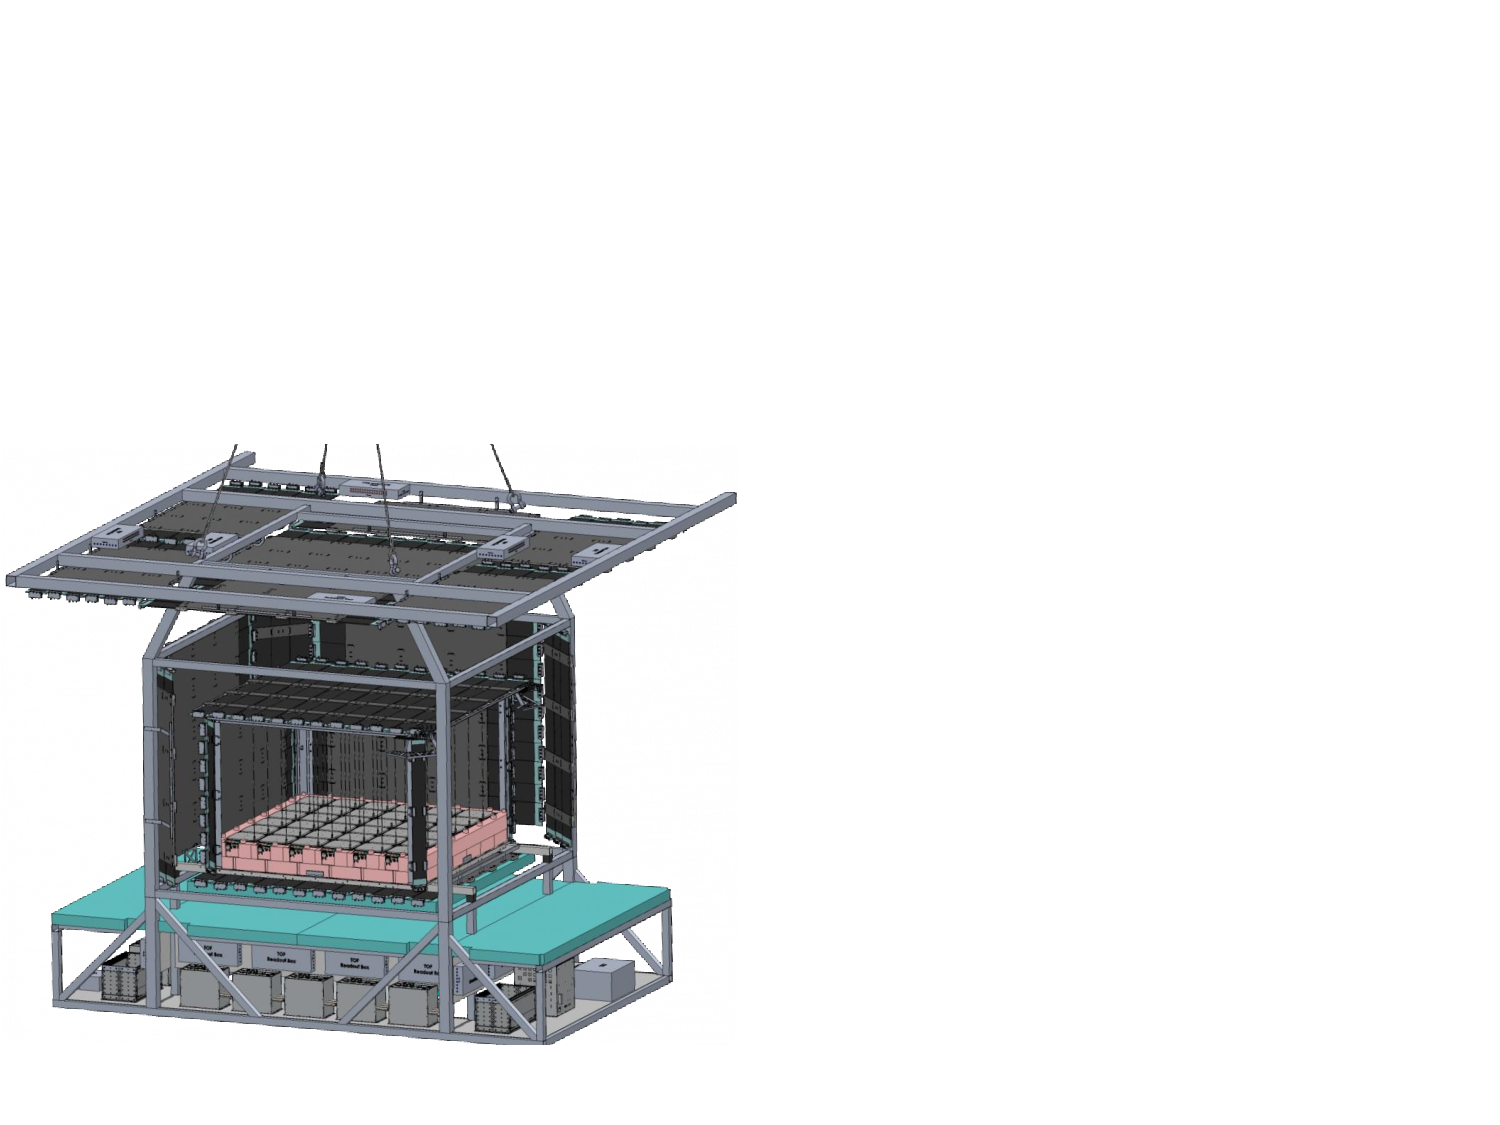
\includegraphics[width=0.95\textwidth]{images/experiment_intro/tracker_menjiao.pdf}
        \end{figure}
        \centering
        
\includegraphics[width=0.8\textwidth]{images/logos/loghi_presentazione.pdf}
    \end{columns}
\end{frame}


%---------------------------------------------------------------------------------------
%	Si(Li) tracker structure
%---------------------------------------------------------------------------------------

\begin{frame}{Si(Li) tracker structure}
    \fontsize{9pt}{1}\selectfont
    \settowidth{\leftmargini}{\usebeamertemplate{enumerate item}}
    \addtolength{\leftmargini}{\labelsep}
    \vspace{0.1cm}
    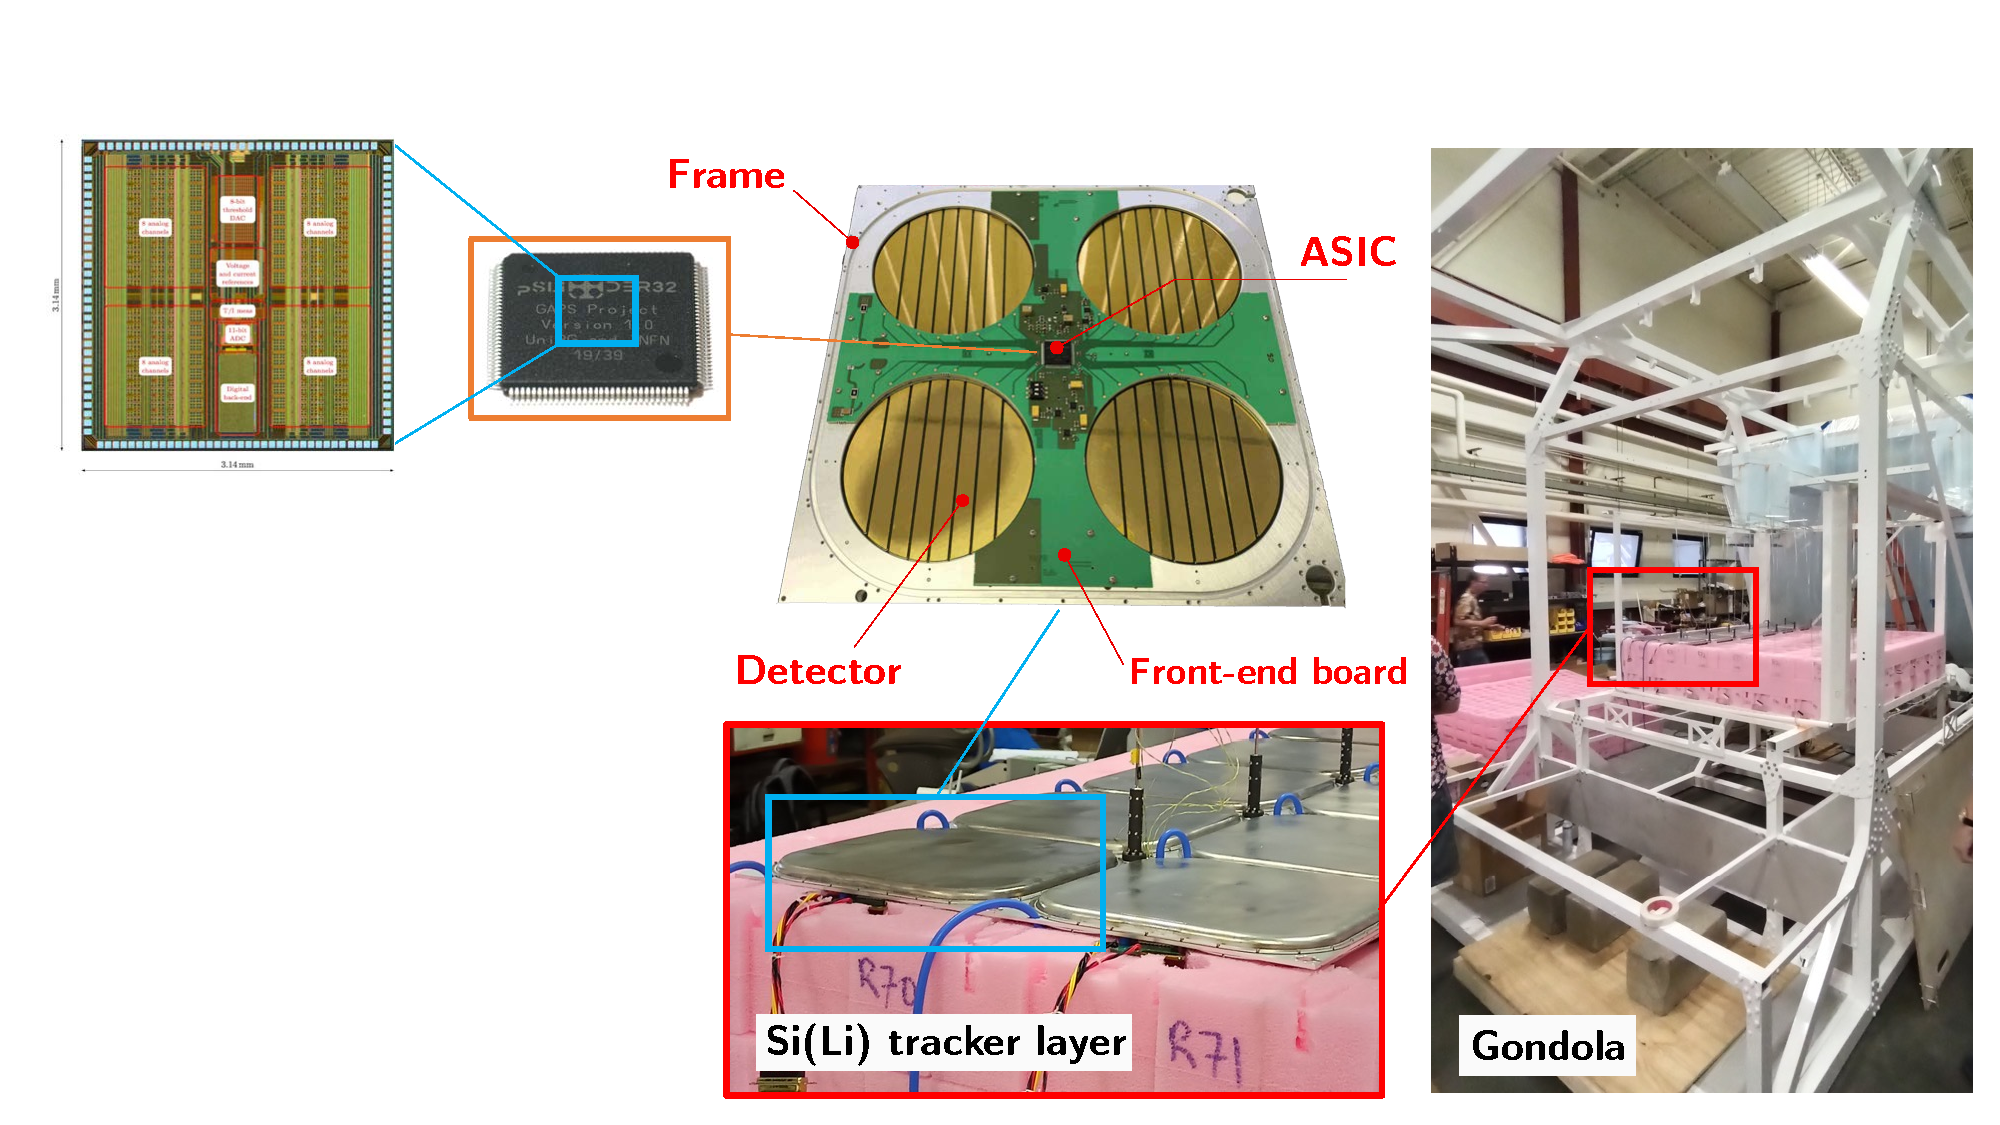
\includegraphics[width=0.99\textwidth]{images/experiment_intro/manghisoni_SIE_ASSEMBLY.pdf}
    \begin{textblock*}{0.35\textwidth}(0.5cm, 4.2cm)
        \textbf{\textcolor{ForestGreen}{Module}}
        \fontsize{8.5pt}{1}\selectfont
        \vspace{0.05cm}
        \begin{itemize}
            \item 1 readout ASIC
            \item 1 Front-End Board (FEB)
            \item 4 Si(Li) detectors (8 strips each)
        \end{itemize}
        \vspace{0.1cm}
        \fontsize{9pt}{1}\selectfont
        \textbf{\textcolor{ForestGreen}{Front-end electronics requirements}}
        \fontsize{8.5pt}{1}\selectfont
        \vspace{0.05cm}
        \begin{itemize}
            \item Channels per ASIC: \textbf{32}
            \item Operating temperature: \textbf{\SI{-40}{\celsius}}
            \item Power dissipation: $\leq$ \textbf{\SI{10}{\milli\watt/ch}}
            \item Dynamic range: \textbf{\SI{10}{\kilo\electronvolt} - \SI{100}{\mega\electronvolt}}
            \item Analog resolution: \textbf{\SI{4}{\kilo\electronvolt} (FWHM)}
            \item Threshold: \textbf{\SI{20}{\kilo\electronvolt}}
        \end{itemize}
    \end{textblock*}
\end{frame}


%---------------------------------------------------------------------------------------
%	SOMMARIO
%---------------------------------------------------------------------------------------

% SOMMARIO (\tableofcontents)
\begin{frame}{Thesis work: overview}
    \settowidth{\leftmargini}{\usebeamertemplate{enumerate item}}
    \addtolength{\leftmargini}{\labelsep}
    \begin{columns}
        \column{0.6\textwidth}
        \vspace{-0.2cm}
        \fontsize{11pt}{1}\selectfont
        \pause
        \begin{enumerate}
            \setlength\itemsep{1em}
            \fontsize{10pt}{1}\selectfont
            \item \textbf{Evaluation of temperature effects on ASIC performance}
            \begin{itemize}
                \fontsize{8.5pt}{1}\selectfont
                \setlength\itemsep{0.3em}
                \item Current reference
                \item Input-output channel trans-characteristic
                \item Global threshold voltage
                \item Equivalent Noise Charge at \SI{-40}{\celsius}
            \end{itemize}\pause
            \fontsize{10pt}{1}\selectfont
            \item \textbf{Si(Li) tracker flight components validation}
            \begin{itemize}
                \fontsize{8.5pt}{1}\selectfont
                \setlength\itemsep{0.3em}
                \item Front-End Boards
                \item Dummy-1 front-end boards
                \item Flex-rigid boards
                \item Connectors for termination
                \item Front-end board shields
            \end{itemize}\pause
            \fontsize{10pt}{1}\selectfont
            \item \textbf{X-ray and particle detection with an assembled Si(Li) tracker module}
            \begin{itemize}
                \fontsize{8.5pt}{1}\selectfont
                \setlength\itemsep{0.3em}
                \item X-ray detection with an Americium 241 source
                \item Cosmic muon detection using an external scintillator
            \end{itemize}
        \end{enumerate}
        \column{0.3\textwidth}
        \centering
        \vskip0.1cm
        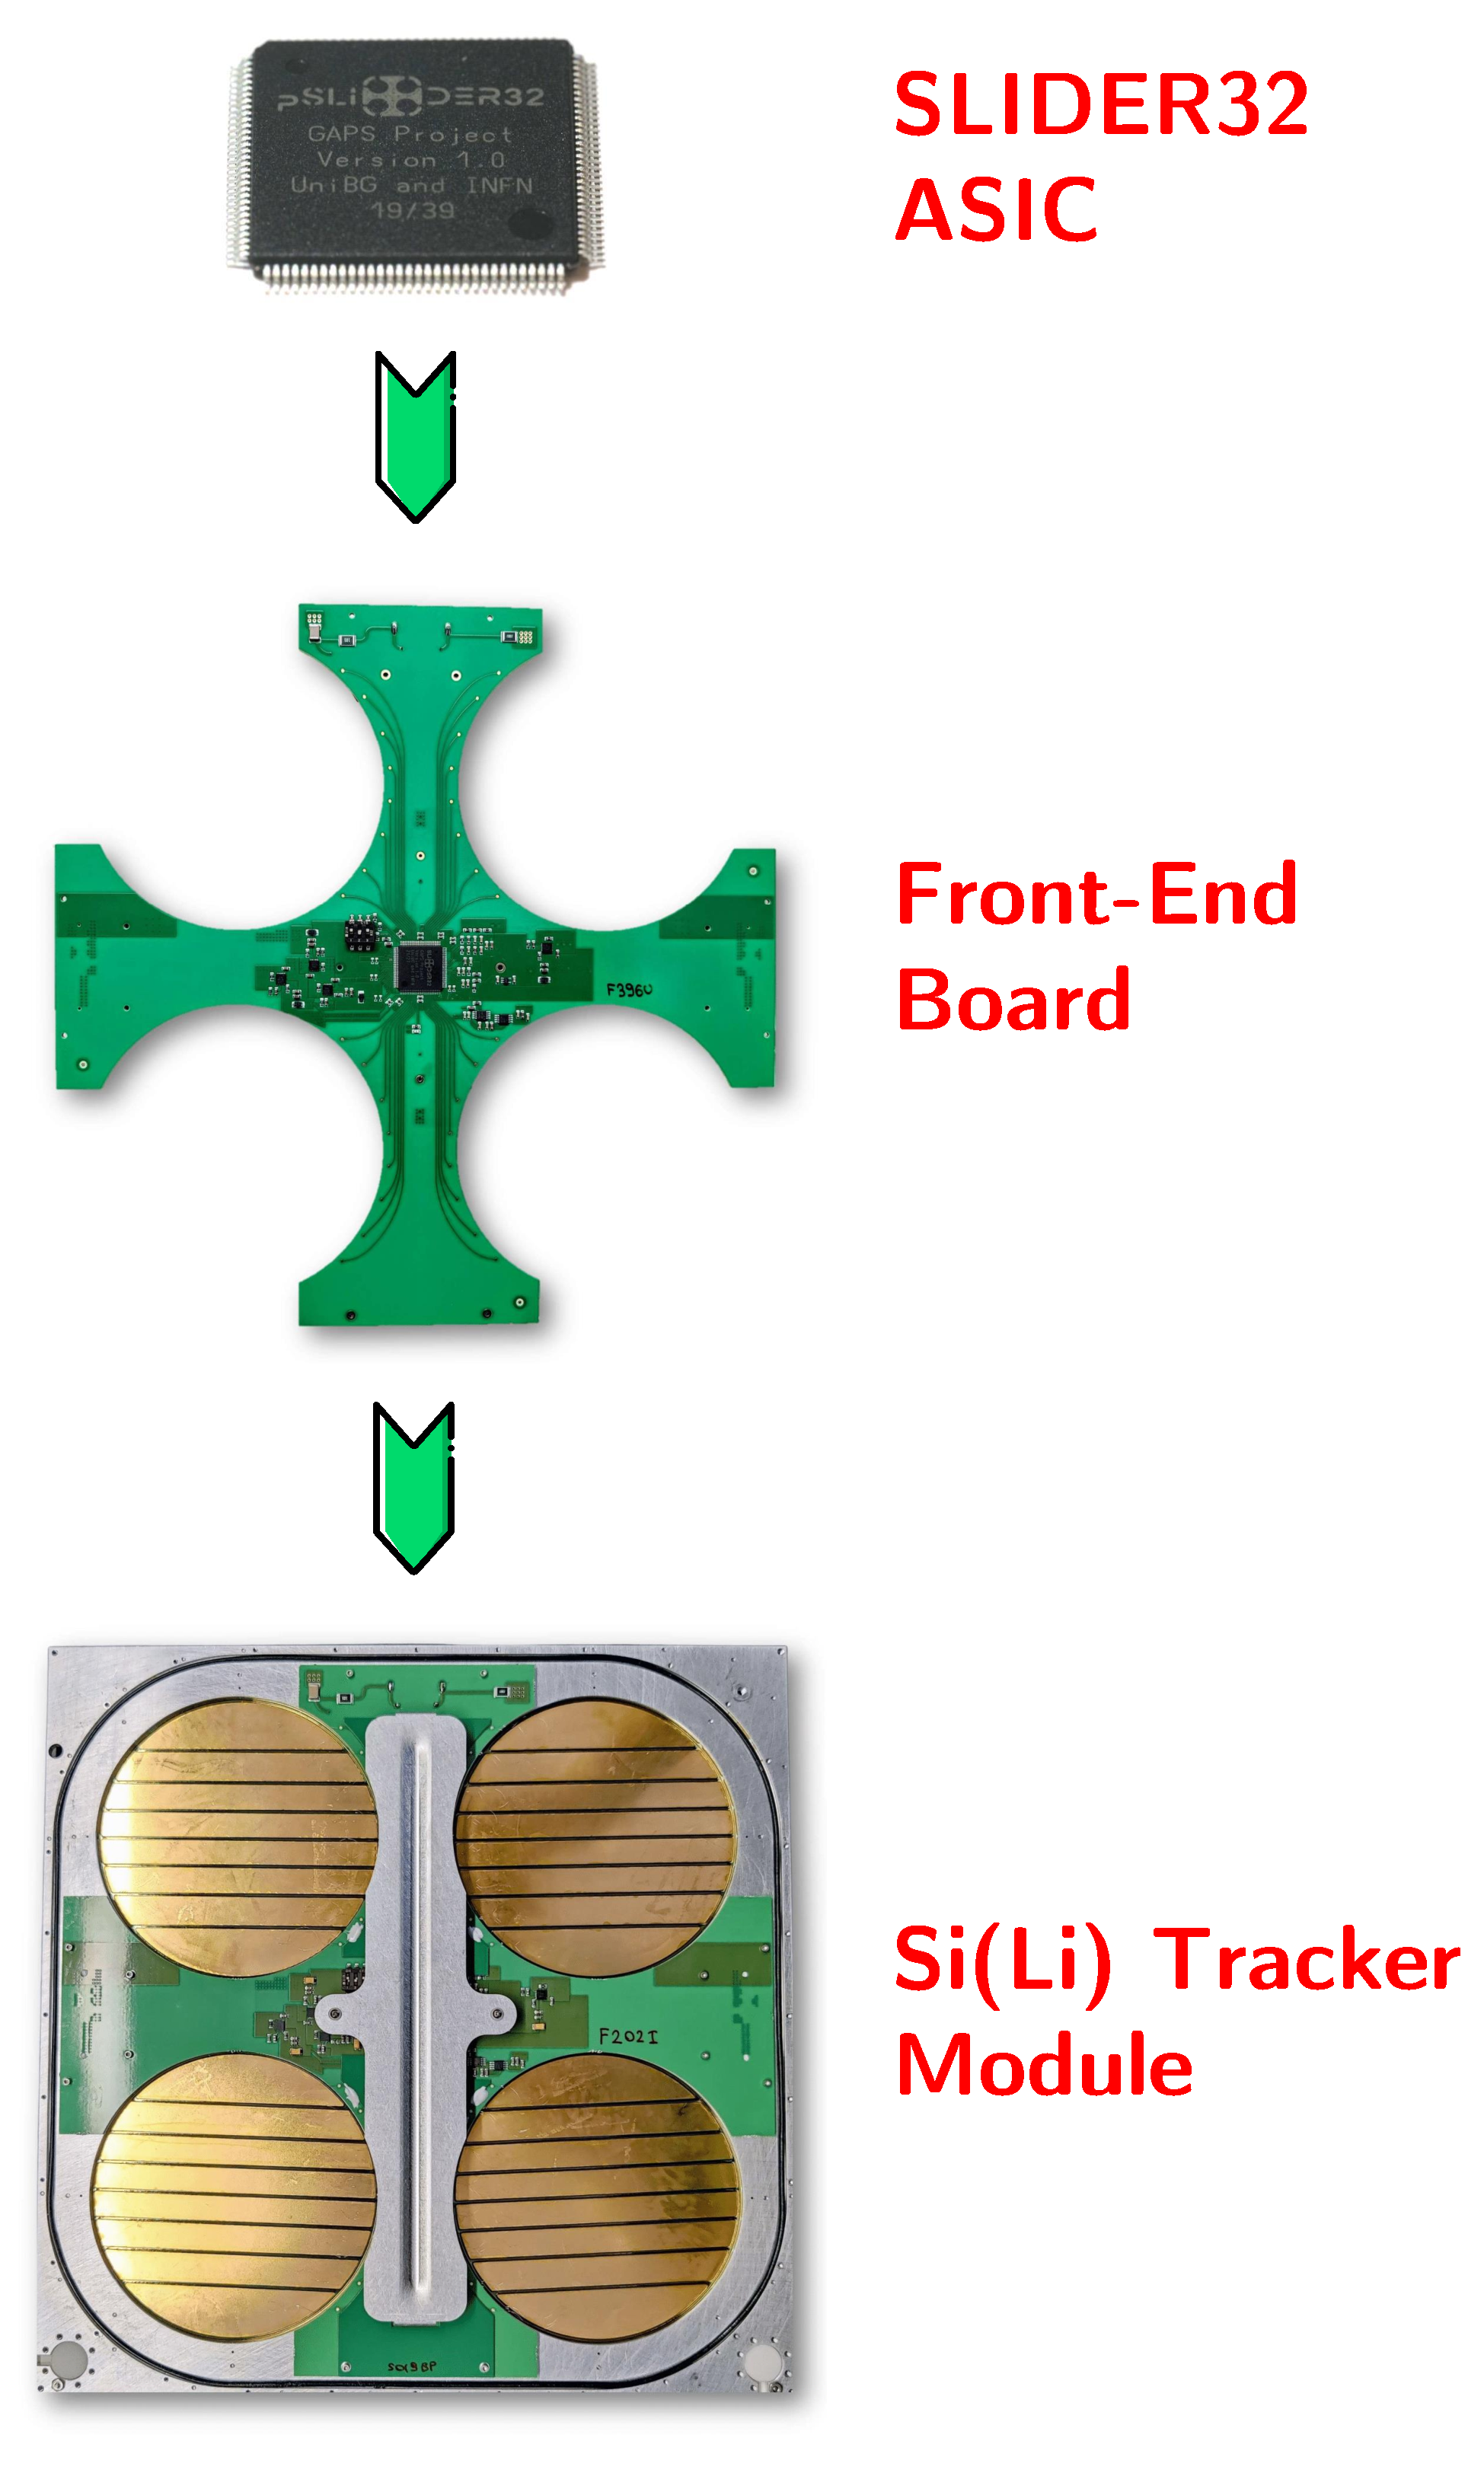
\includegraphics[height=0.85\textheight]{images/random/workflow.pdf}
    \end{columns}
\end{frame}

%---------------------------------------------------------------------------------------
%	ASIC characterisation at different temperatures
%--------------------------------------------------------------------------------------- 

\begin{frame}{ASIC characterisation at different temperatures}
\fontsize{8.5pt}{1}\selectfont
    \begin{columns}[T]
    \column{0.475\textwidth}
        \vskip0.3cm
        \fontsize{9pt}{1}\selectfont
        \textbf{\textcolor{ForestGreen}{SLIDER32 ASIC test setup}}\\
        \vskip0.15cm
        \fontsize{8.5pt}{1}\selectfont
        Tests conducted on the SLIDER32 readout ASIC with a purposely designed test board were aimed at evaluate temperature effects on:
        \begin{enumerate}
            \item \textcolor{Red}{\textbf{Bandgap reference current}}
            \item \textcolor{Red}{\textbf{Channel input-output characteristic}}
            \item \textcolor{Red}{\textbf{DAC for setting the global threshold voltage}}
        \end{enumerate}
        \vskip0.05cm
        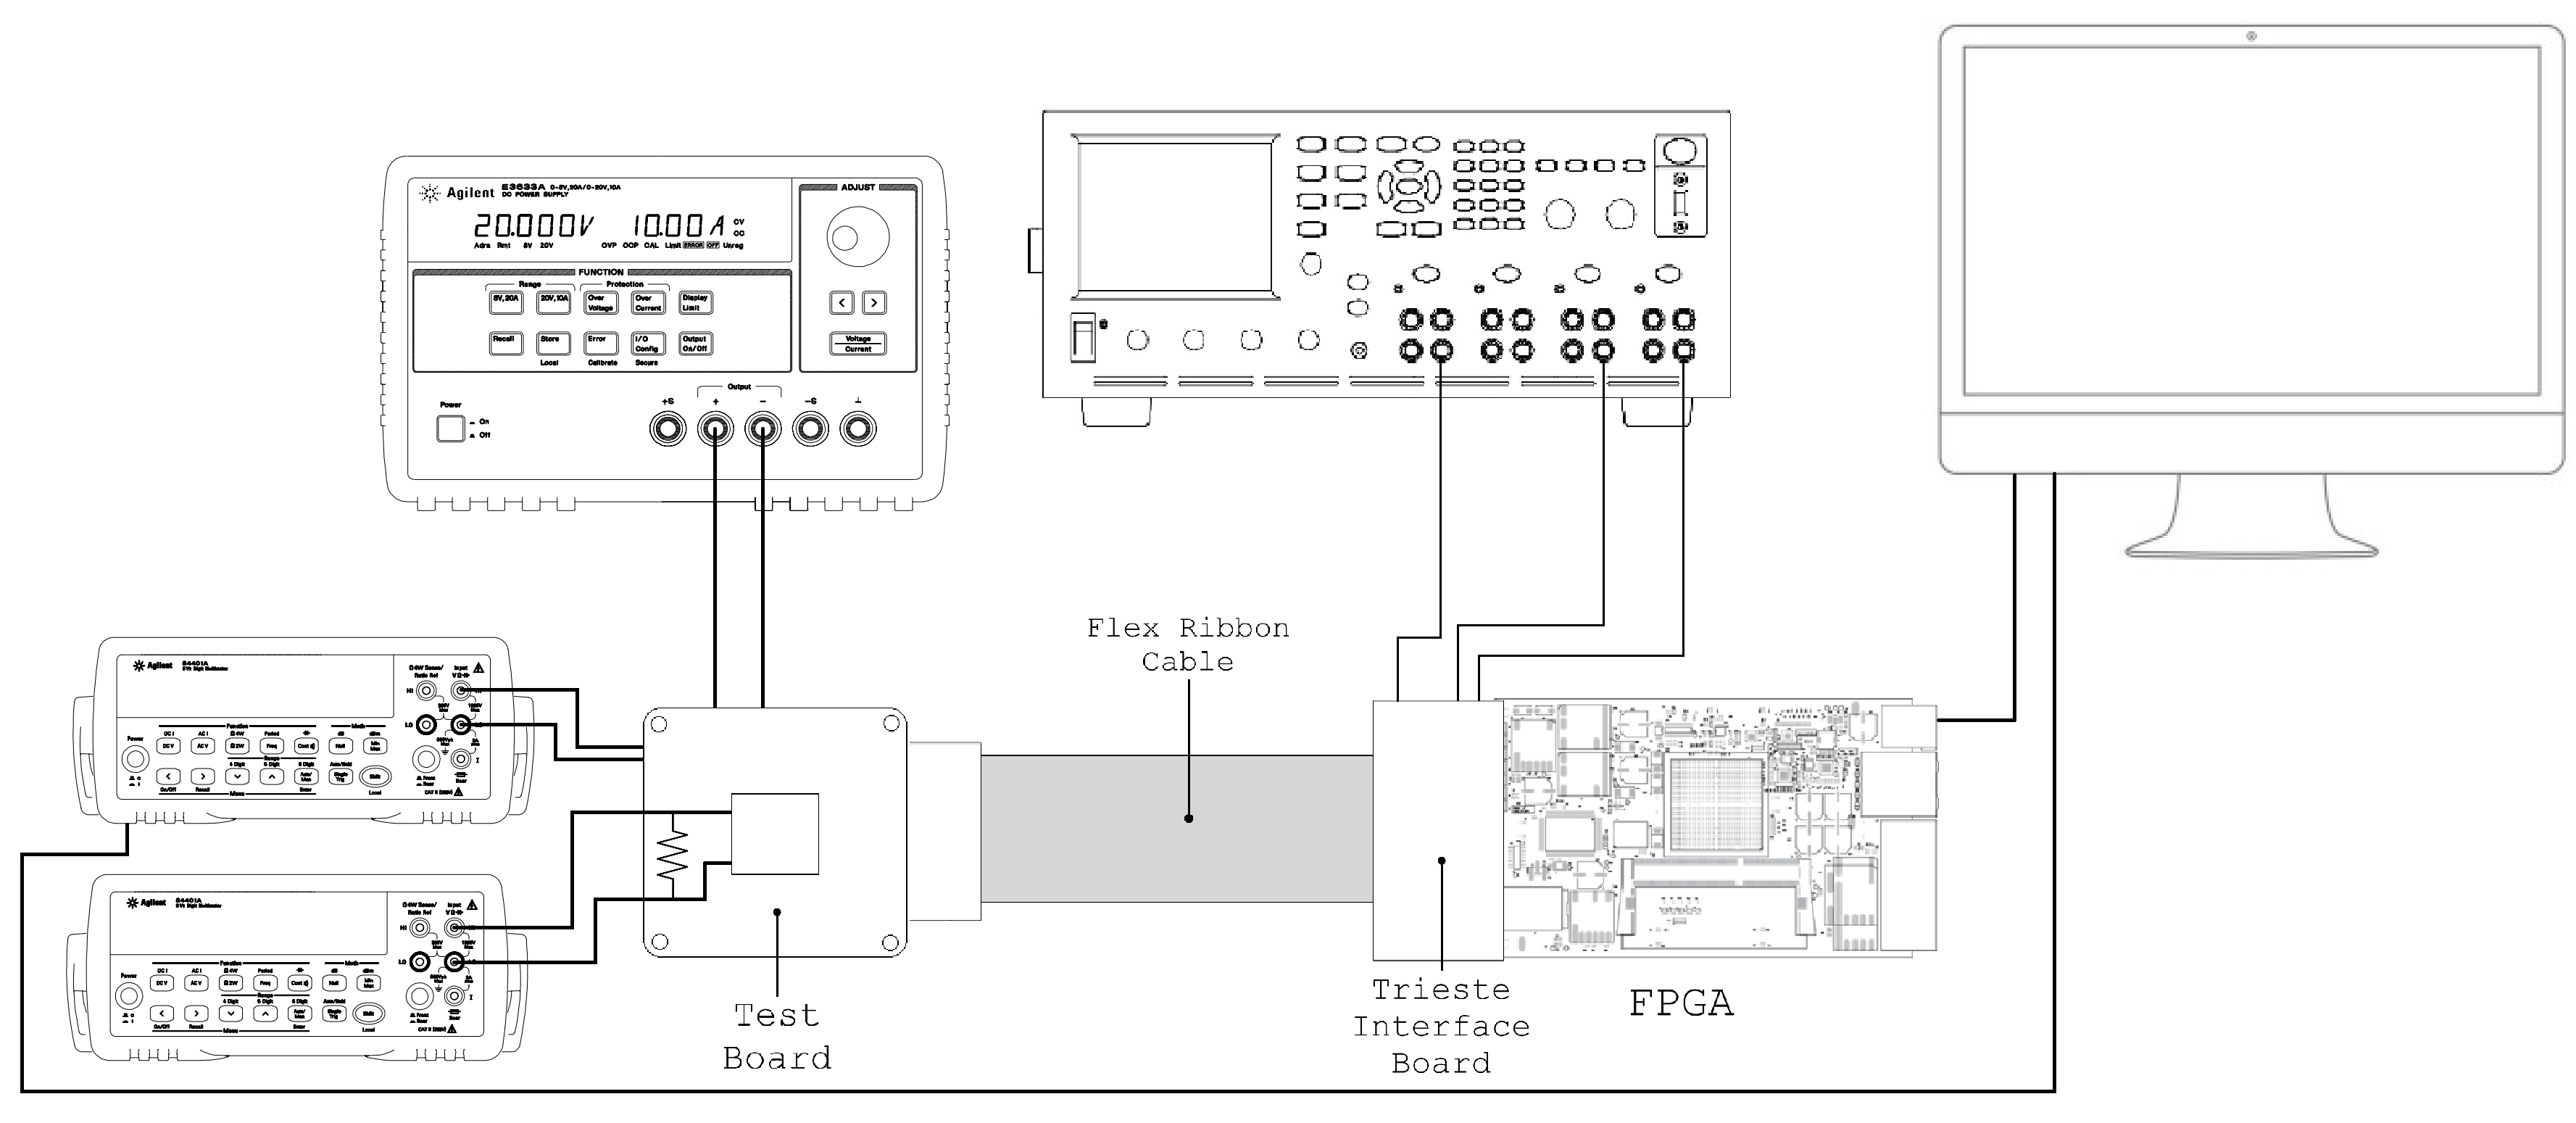
\includegraphics[width=0.95\textwidth]{images/temperature_effects/test_setup_test_board_csavrefgm_530mv.png}
        \vskip0.2cm
        Measurements performed in a temperature controlled environment and temperature range spanning:
        \begin{itemize}
            \item $\SI{-40}{\celsius} \div +\SI{30}{\celsius}$ with \SI{10}{\celsius} steps
            \item $\SI{-40}{\celsius} \div \SI{-30}{\celsius}$ with \SI{2}{\celsius} steps
        \end{itemize}
    \column{0.475\textwidth}
        \settowidth{\leftmargini}{\usebeamertemplate{itemize item}}
        \addtolength{\leftmargini}{\labelsep}
        \vskip0.3cm
        \fontsize{9pt}{1}\selectfont
        \textbf{\textcolor{ForestGreen}{Bandgap reference current}}\\
        \vskip0.15cm
        \fontsize{8.5pt}{1}\selectfont
        Adjustable current reference by means of 3 bits (\texttt{BBB}) and \textbf{\SI{5}{\micro\ampere}} nominal value
        \vskip-0.4cm
        \begin{center}
            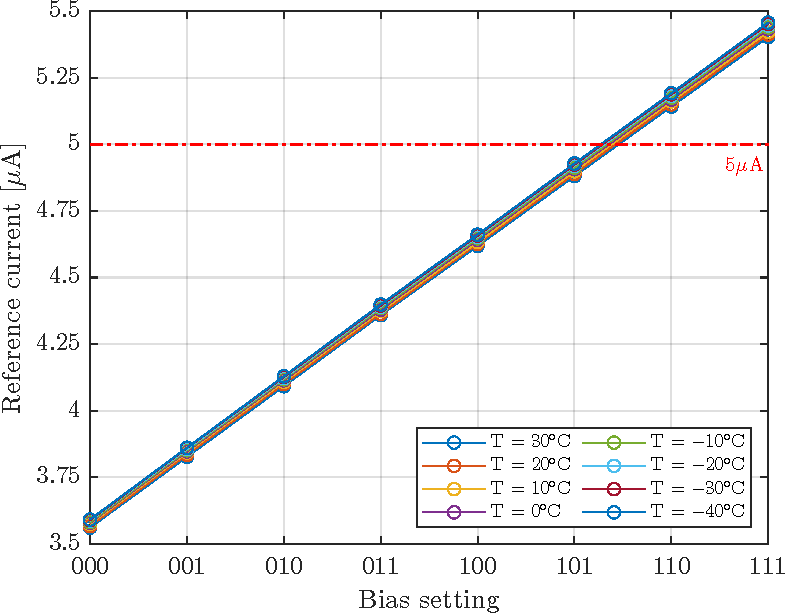
\includegraphics[height=0.5\textheight]{images/temperature_effects/BGR_current_XBBB.pdf}
        \end{center}
        \vskip-0.2cm
        \begin{itemize}
            \item \SI{5}{\micro\ampere} nominal value obtained with \texttt{BBB} = $(\texttt{101})_{2}$ and \textbf{$\approx\SI{1.86}{\percent}$} error on avarage \greencheck 
            \item \textbf{$< \SI{1}{\percent}$} variation between \SI{-40}{\celsius} and \SI{30}{\celsius} for the same \texttt{BBB} bits configuration \greencheck
        \end{itemize}
    \end{columns}
\end{frame}


%---------------------------------------------------------------------------------------
%	Channel input-output characteristic
%---------------------------------------------------------------------------------------

\begin{frame}{Channel input-output characteristic}
\fontsize{8.5pt}{1}\selectfont
    \vspace{-0.15cm}
    \begin{columns}
    \column{0.32\textwidth}
        \settowidth{\leftmargini}{\usebeamertemplate{itemize item}}
        \addtolength{\leftmargini}{\labelsep}

        \begin{itemize}
            \item Charge Sensitive Amplifier (CSA) based on an inverting gain stage and a feedback capacitor
            \item \textbf{Dynamic signal compression} achieved by implementing the feedback capacitor with an NMOSFET $\rightarrow$ channel gain dependent on incoming energy
        \end{itemize}

        \begin{center}
             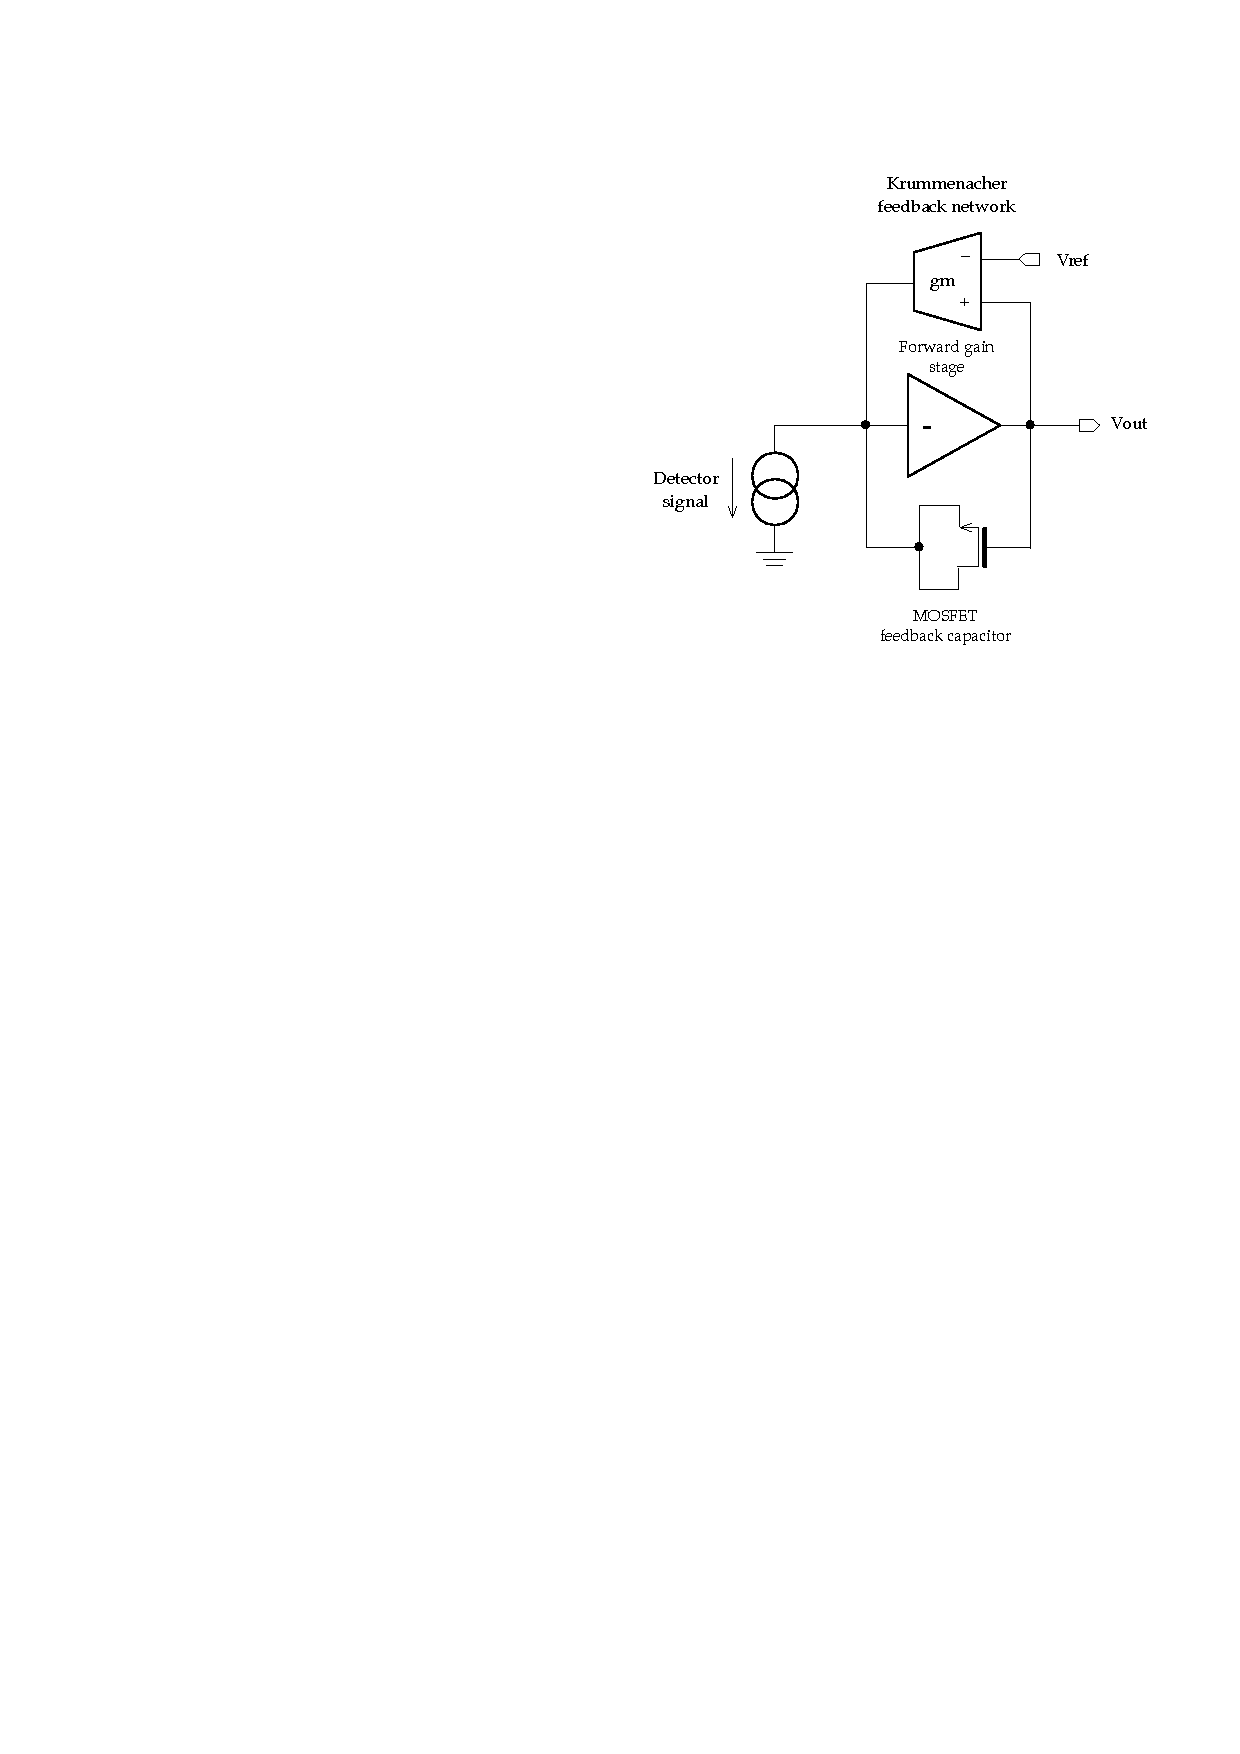
\includegraphics[height=0.52\textheight]{images/temperature_effects/CSA_schematic.pdf}
        \end{center}

        \column{0.65\textwidth}
            \settowidth{\leftmargini}{\usebeamertemplate{itemize item}}
            \addtolength{\leftmargini}{\labelsep}
            \begin{center}
                \fontsize{9pt}{1}\selectfont
                \textcolor{ForestGreen}{\textbf{\texttt{CSAVrefGM} voltage: automatically regulated vs fixed to \SI{530}{\milli\volt}}}\\
            \end{center}
            \fontsize{8.5pt}{1}\selectfont
            \begin{center}
                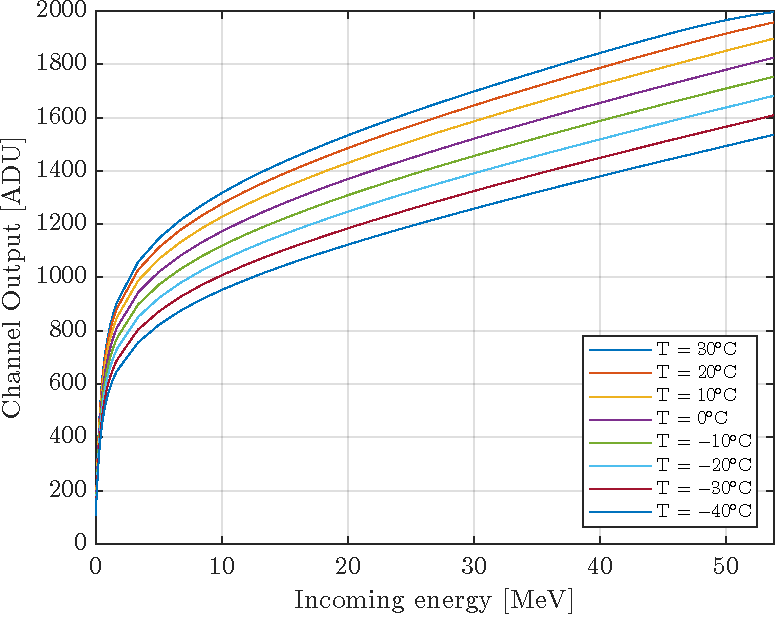
\includegraphics[height=0.42\textheight]{images/temperature_effects/fdt_csavrefgm_auto_tau6_keV_0011.pdf}
                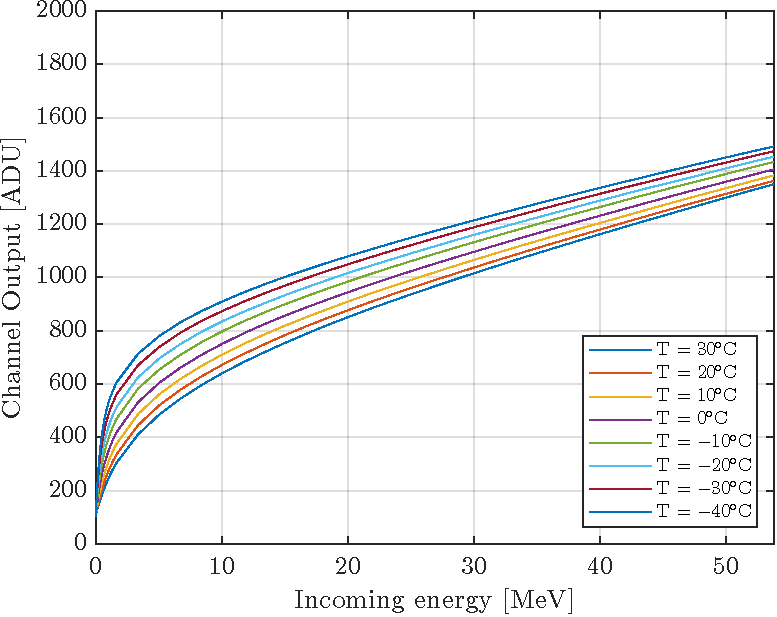
\includegraphics[height=0.42\textheight]{images/temperature_effects/fdt_csavrefgm_530mV_tau6_keV.pdf}
            \end{center}    
            \vskip-0.2cm
            \begin{itemize}
                \item Injected charge spanning from \textbf{0} to \textbf{\SI{55.11}{\mega\electronvolt}} \greencheck
                \item Both configurations successfully tested and channel characteristic performing as expected at every temperature step \greencheck
            \end{itemize}
            \vskip0.3cm
            Channel gain studied in two energy regions:
            \begin{itemize}
                \item \textbf{\textcolor{Red}{Low energy region}}: X-ray detection region ranging from \textbf{0} to \textbf{\SI{100}{\kilo\electronvolt}}
                \item \textbf{\textcolor{Red}{High energy region}}: Muon detection region, ranging from \textbf{40} to \textbf{\SI{55}{\mega\electronvolt}}
            \end{itemize}
            \vspace{0.4cm}
    \end{columns}
\end{frame}


%---------------------------------------------------------------------------------------
%	Gain and kink as function of temperature
%---------------------------------------------------------------------------------------

\begin{frame}{Gain and kink as function of temperature}
\fontsize{8.5pt}{1}\selectfont
    \begin{columns}
    \column{0.42\textwidth}
        \settowidth{\leftmargini}{\usebeamertemplate{itemize item}}
        \addtolength{\leftmargini}{\labelsep}

        
        Channel transfer function roughly approximated by two linear models:
        
        \vspace{0.3cm}
        \begin{equation*}
            y = p + g \cdot x
        \end{equation*}

        \vspace{-0.1cm}
        where:
        \vspace{0.1cm}
        
        \begin{itemize}
            \itemsep0em
            \item \textbf{y} [\SI{}{ADU}] (Analog Digital Unit): channel output
            \item \textbf{p} [\SI{}{ADU}]: pedestal, repeated sampling of the channel output without charge injected
            \item \textbf{g} [\SI{}{ADU/\kilo\electronvolt}]: channel gain
            \item \textbf{x} [\SI{}{\kilo\electronvolt}]: input energy
        \end{itemize}
        \vspace{-0.1cm}
        \begin{center}
            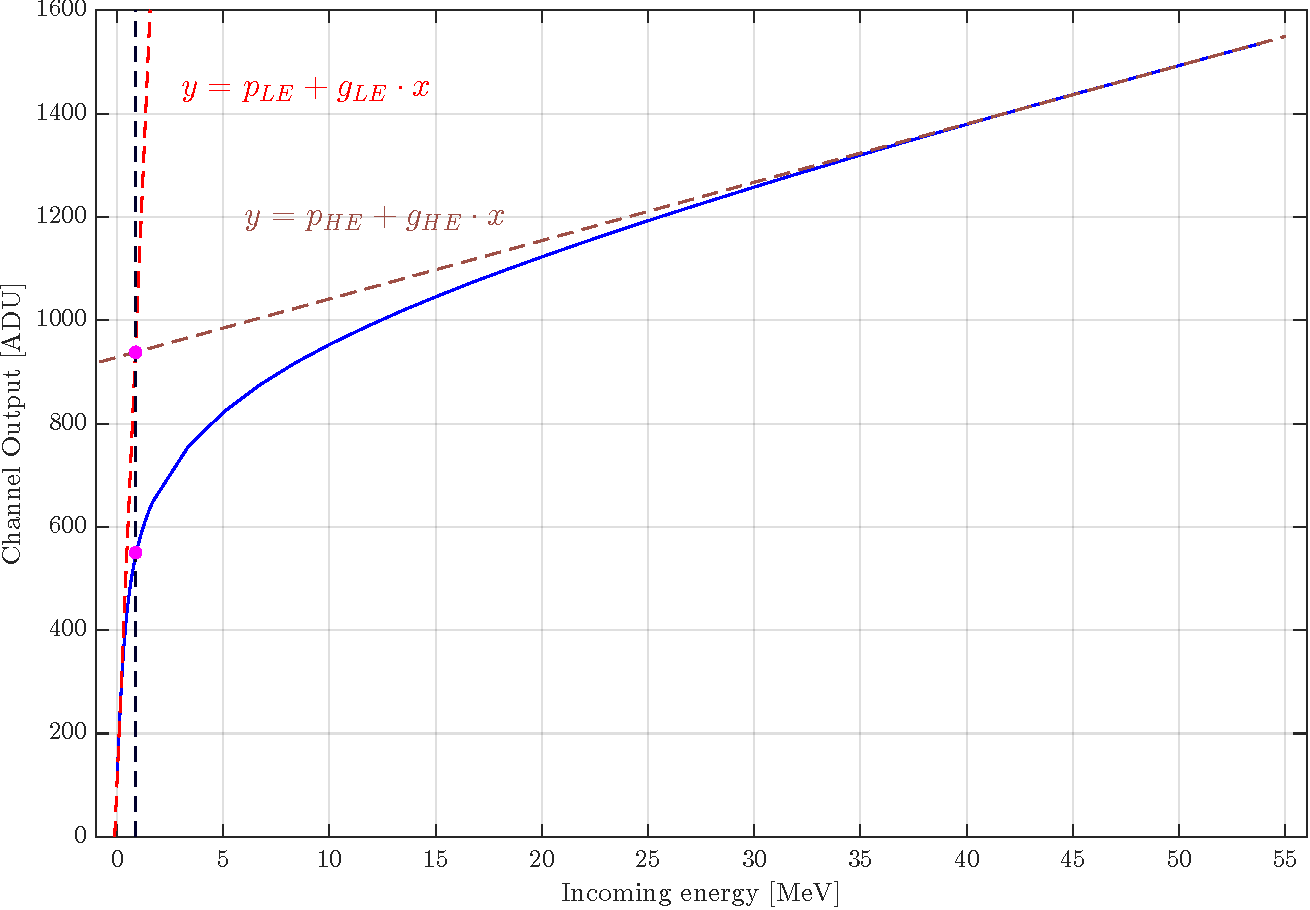
\includegraphics[height=0.4\textheight]{images/temperature_effects/fdt_calcolo_kink.pdf}
        \end{center}
        \vspace{0.05cm}
        
        \column{0.53\textwidth}
            \vspace{-0.3cm}
            \begin{center}
                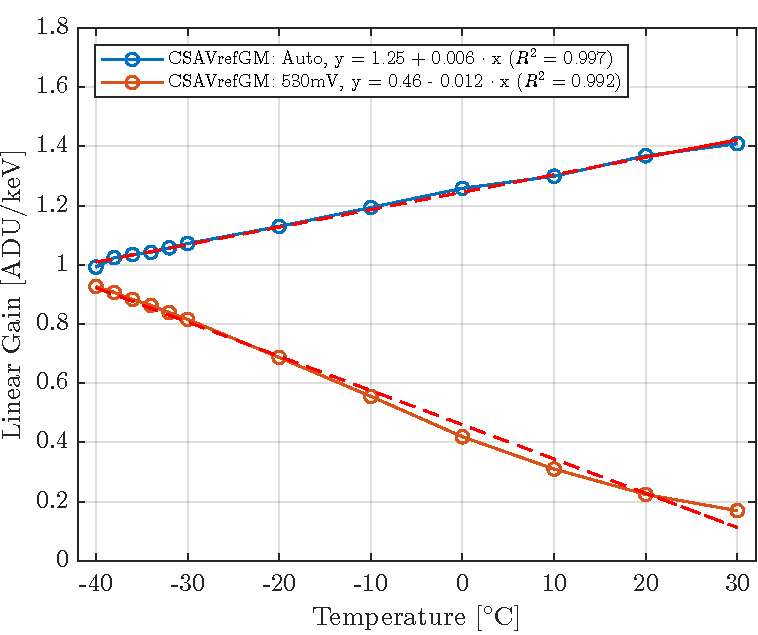
\includegraphics[width=0.488\textwidth]{images/temperature_effects/low_energy_gain_auto_530mV.pdf}
                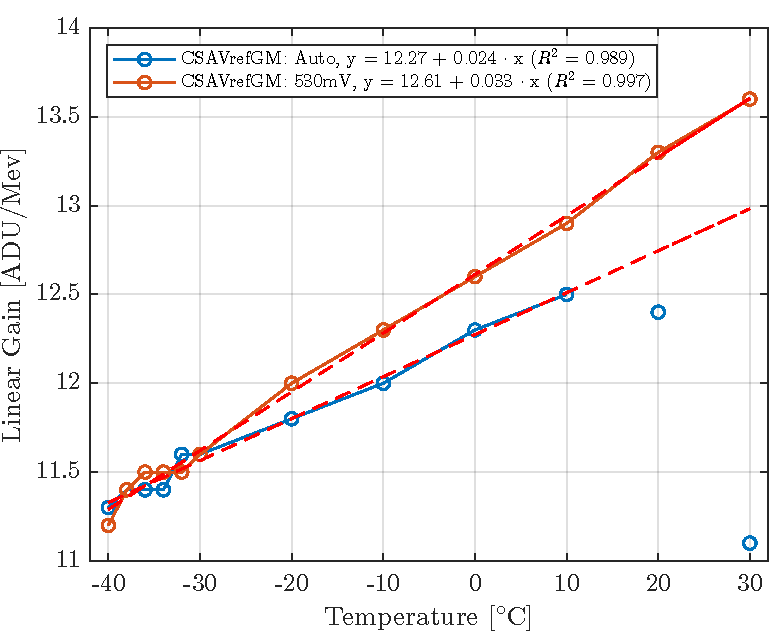
\includegraphics[width=0.498\textwidth]{images/temperature_effects/high_energy_gain_auto_530mV.pdf}
            \end{center}

            \vskip-0.3cm
            \settowidth{\leftmargini}{\usebeamertemplate{itemize item}}
            \addtolength{\leftmargini}{\labelsep}
            \begin{itemize}
                \item Low energy gain decreases with fixed reference voltage \redcross
                \item Temperature effects compensated with variable voltage reference \greencheck
            \end{itemize}
            \vskip0.1cm

            \begin{columns}
                \settowidth{\leftmargini}{\usebeamertemplate{itemize item}}
                \addtolength{\leftmargini}{\labelsep}
                \column{0.4\textwidth}
                    \vskip0.1cm
                    \centering
                    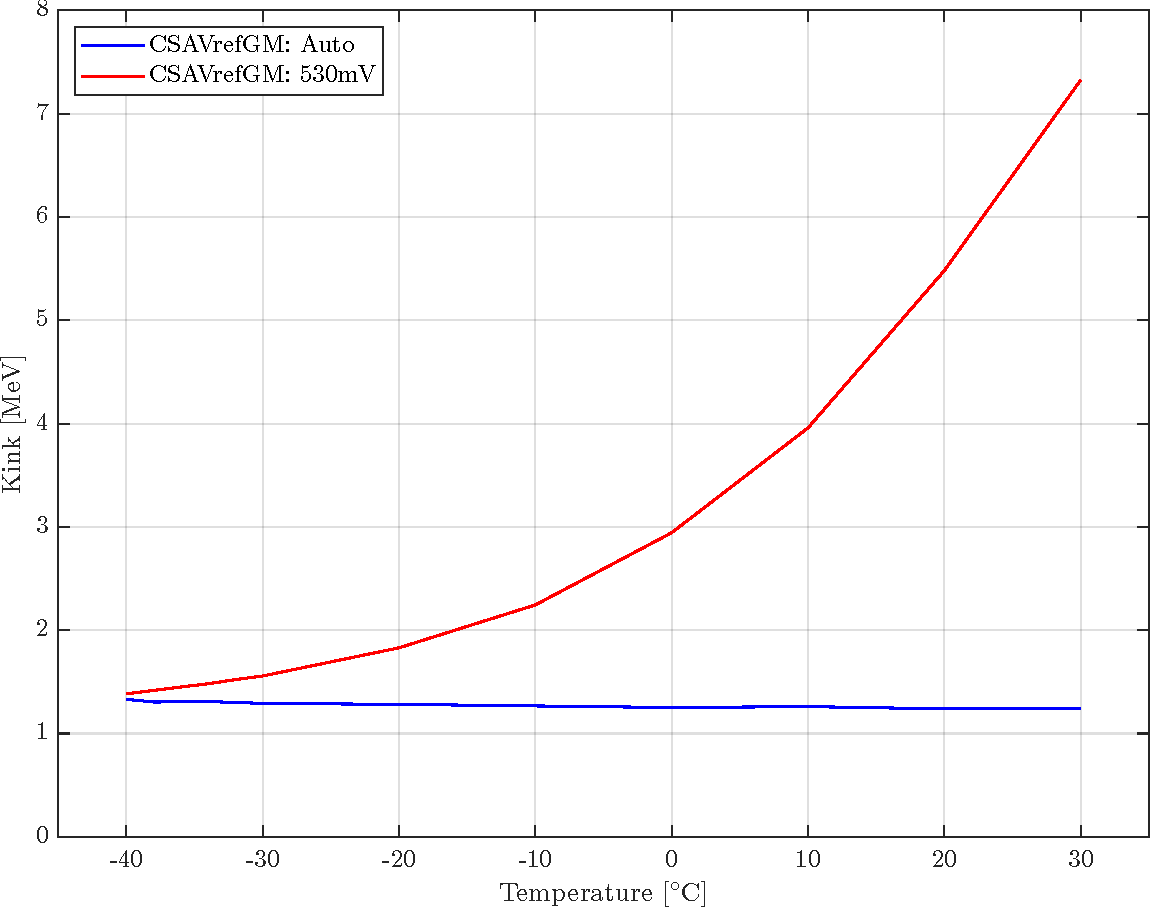
\includegraphics[width=1.1\textwidth]{images/temperature_effects/plot_pedestal_gain_auto_530mV.pdf}
                    
                \column{0.5\textwidth}
                    \textcolor{ForestGreen}{\textbf{Kink trend as function of temperature}}
                    \vspace{0.1cm}
                    \begin{itemize}
                        \item Kink in \textbf{\SI{1.28}{\mega\electronvolt}} @ \SI{-40}{\celsius}
                        \item \textbf{\SI{6.95}{\percent}} variation with variable reference voltage \greencheck
                        \item \textbf{\SI{429}{\percent}} variation with fixed reference voltage \redcross
                    \end{itemize}
            \end{columns}
            \vspace{0.5cm}
    \end{columns}
\end{frame}


%---------------------------------------------------------------------------------------
%	Si(Li) tracker flight components validation
%---------------------------------------------------------------------------------------

\begin{frame}{Si(Li) tracker flight components}
    \vskip0.1cm
    \centering
    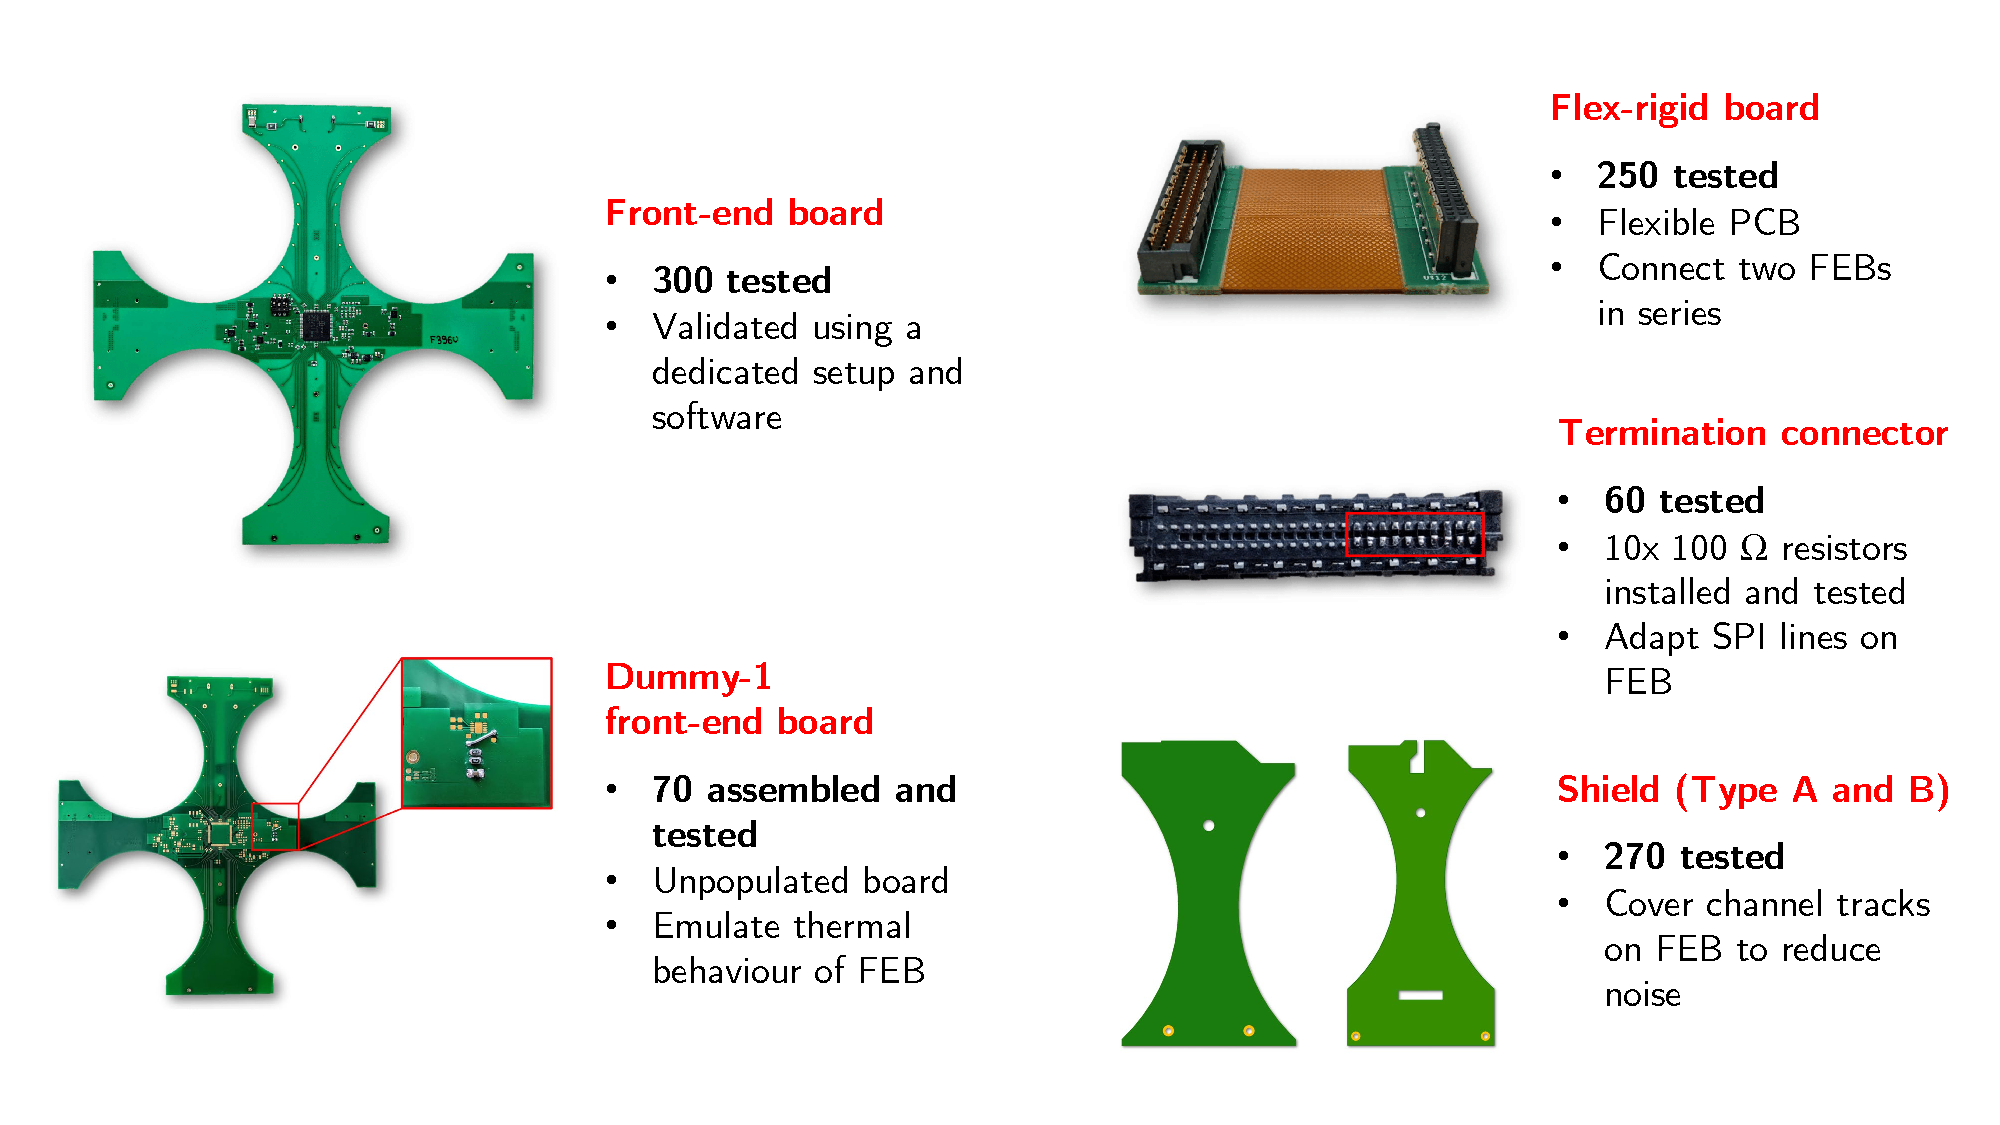
\includegraphics[width=1.01\textwidth]{images/flight_components_validation/flight_items_recap.pdf}
\end{frame}


%---------------------------------------------------------------------------------------
%	Si(Li) tracker flight components validation
%---------------------------------------------------------------------------------------

\begin{frame}{Si(Li) tracker flight components validation}
    \fontsize{8.5pt}{1}\selectfont
    \begin{columns}
        \column{0.52\textwidth}
        \textbf{\large \textcolor{ForestGreen}{Validation procedure}}\\
        \vspace{0.15cm}
        Each item has been subjected to a validation procedure that included:
        \begin{itemize}
            \item \textbf{\textcolor{Red}{Thermal cycle}} if not already performed by the manufacturer
            \item \textbf{\textcolor{Red}{Visual inspection}} to search for defects and missing or bad soldered components
            \item \textbf{\textcolor{Red}{Measurements}} that vary upon the specific flight item
        \end{itemize}
        \vspace{0.2cm}
        At the end of the test procedure:
        \begin{enumerate}
            \item Test results have been saved in a database
            \item An item \textbf{report} with test results has been generated \vspace{-0.18cm}
            \item The item has been classified as
            \begin{itemize}
                \item \textcolor{LimeGreen}{GOOD}
                \item \textcolor{BurntOrange}{USABLE for testing activity only}
                \item \textcolor{OrangeRed}{UNUSABLE}
            \end{itemize}
        \end{enumerate}
        \vspace{0.2cm}
        GOOD and USABLE items have been shipped to \textbf{Columbia University} to be used in the final assembly of the experiment at the \textbf{MIT Bates} facility in Middleton, Massachusetts
        \column{0.42\textwidth}
            \centering
            \vskip0.05cm
            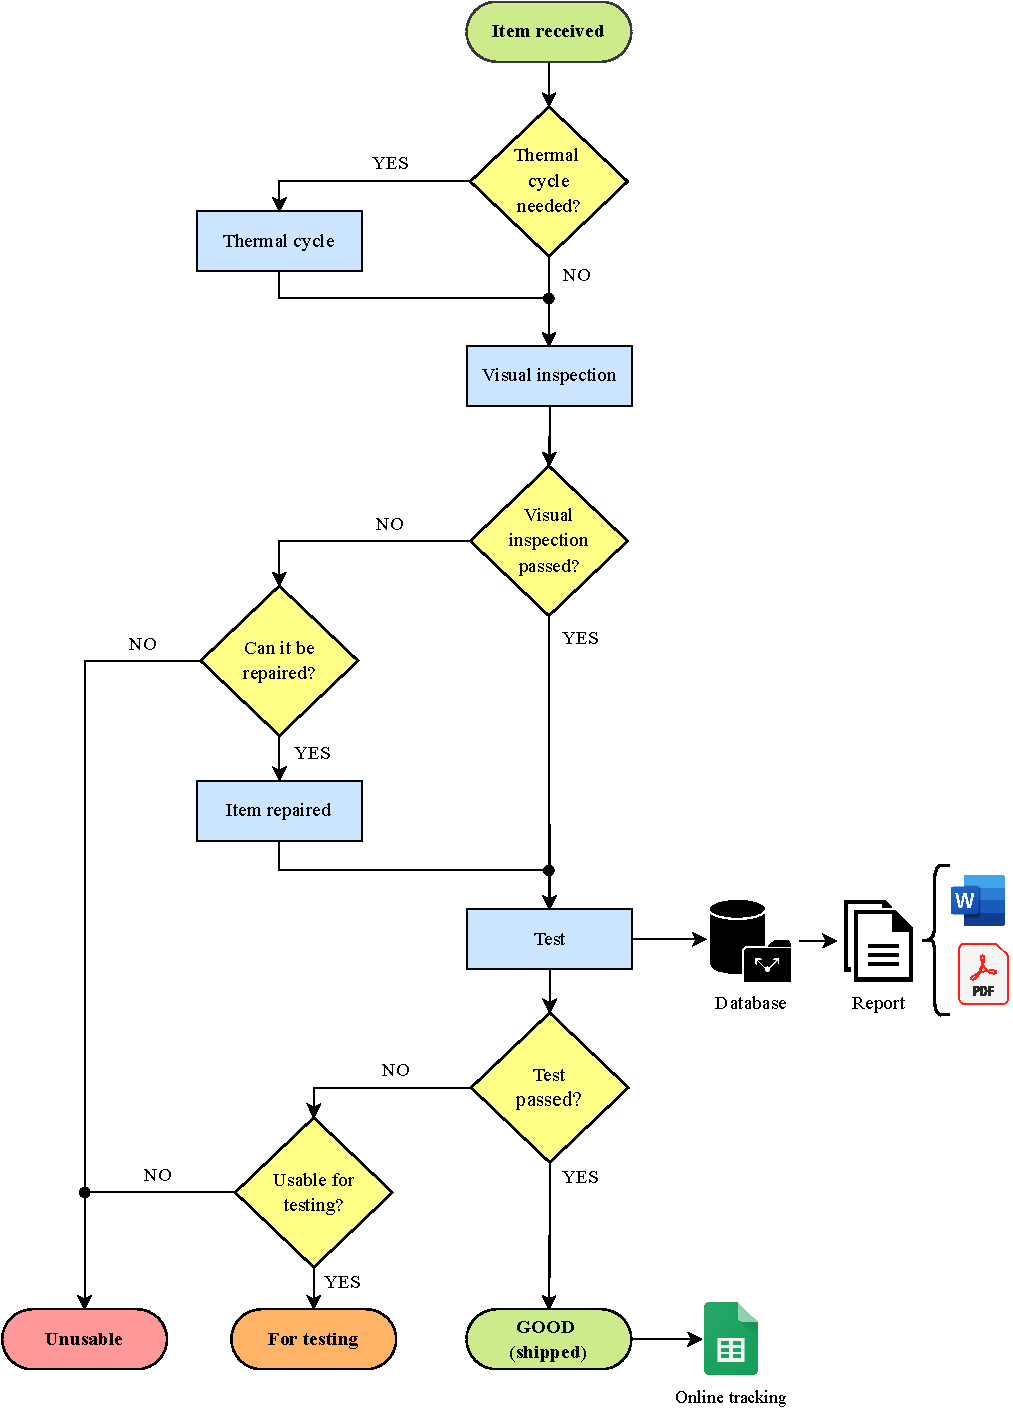
\includegraphics[height=0.86\textheight]{images/flight_components_validation/flight_item_validation_procedure.drawio.pdf}
    \end{columns}
\end{frame}


%---------------------------------------------------------------------------------------
%	Yield and test reports
%---------------------------------------------------------------------------------------

\begin{frame}{Yield and test reports}
    \fontsize{8.5pt}{1}\selectfont
    \begin{columns}
        \column{0.65\textwidth}
            \centering
            \vspace{-0.1cm}
            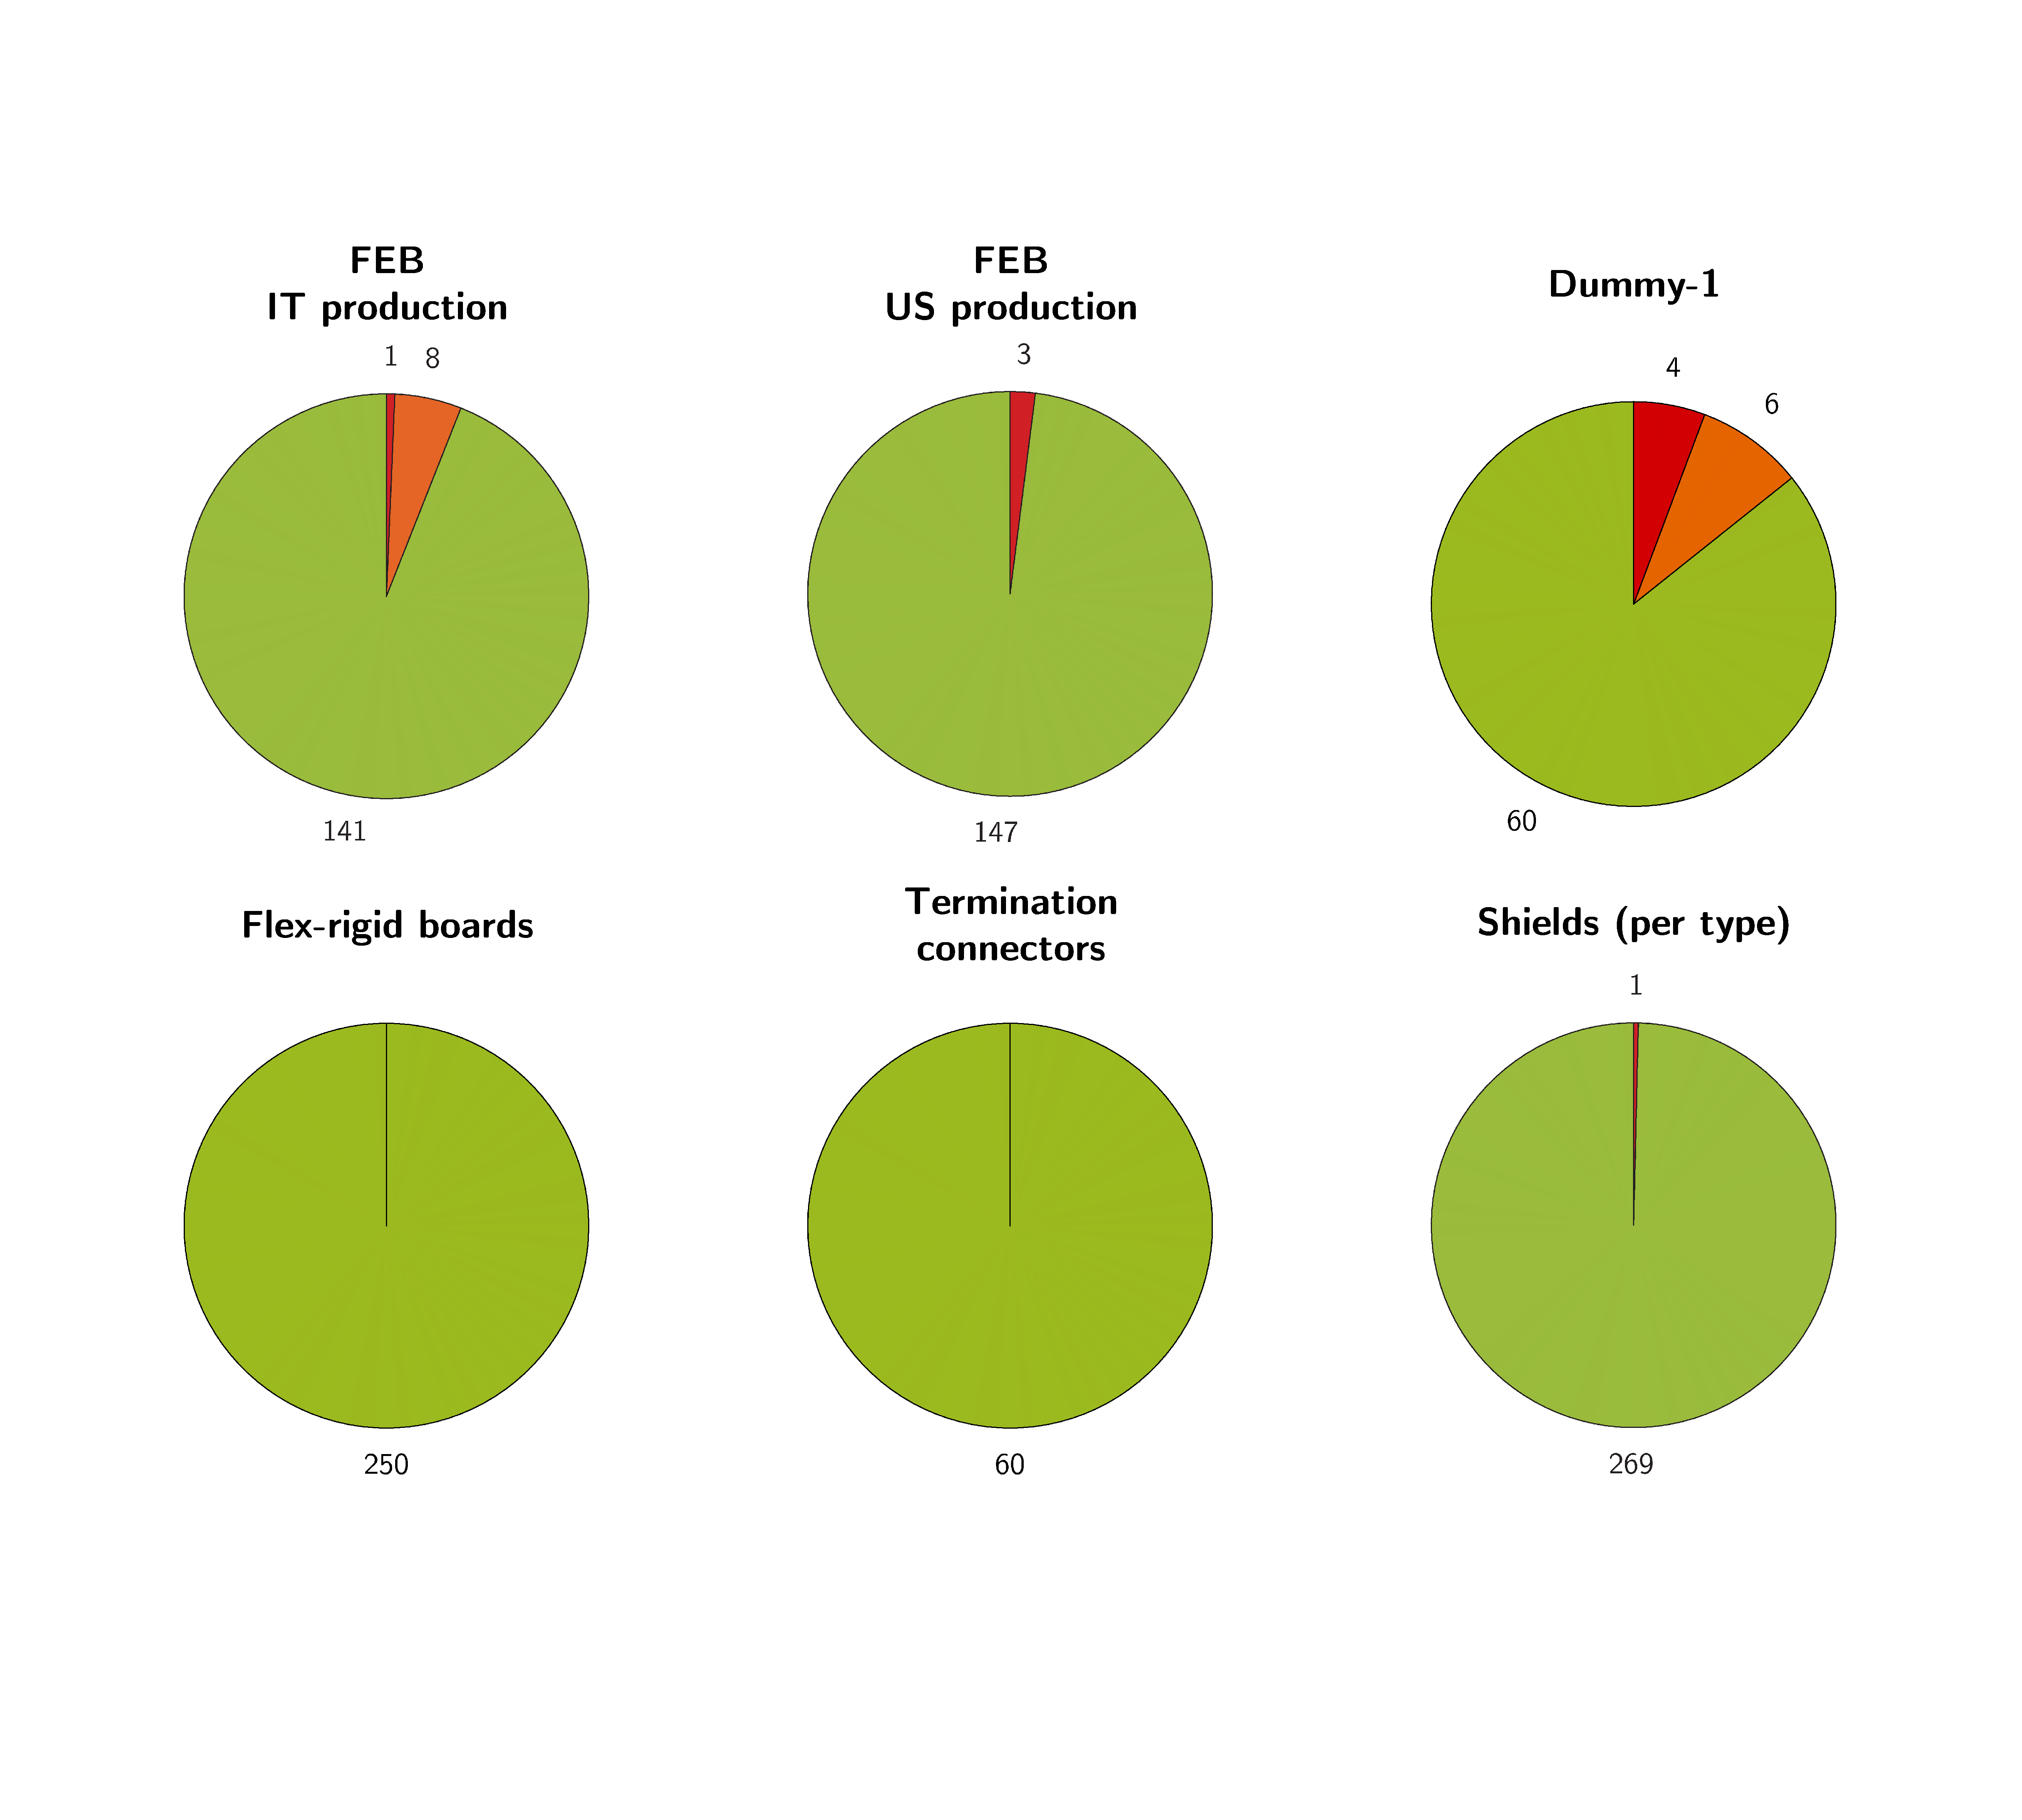
\includegraphics[width=1.05\textwidth]{images/flight_components_validation/yield/item_pies.pdf}
        \column{0.35\textwidth}
            \centering
            \fontsize{10pt}{1}\selectfont
            \textbf{\textcolor{Red}{Test reports}}\\
            \vspace{0.2cm}
            \fontsize{8.5pt}{1}\selectfont
            For every validated flight item,\\ a report has been generated,\\ detailing the most important\\ reference parameters to be later\\ used in the final assembly of the instrument\\
            \vspace{0.3cm}
            \frame{
                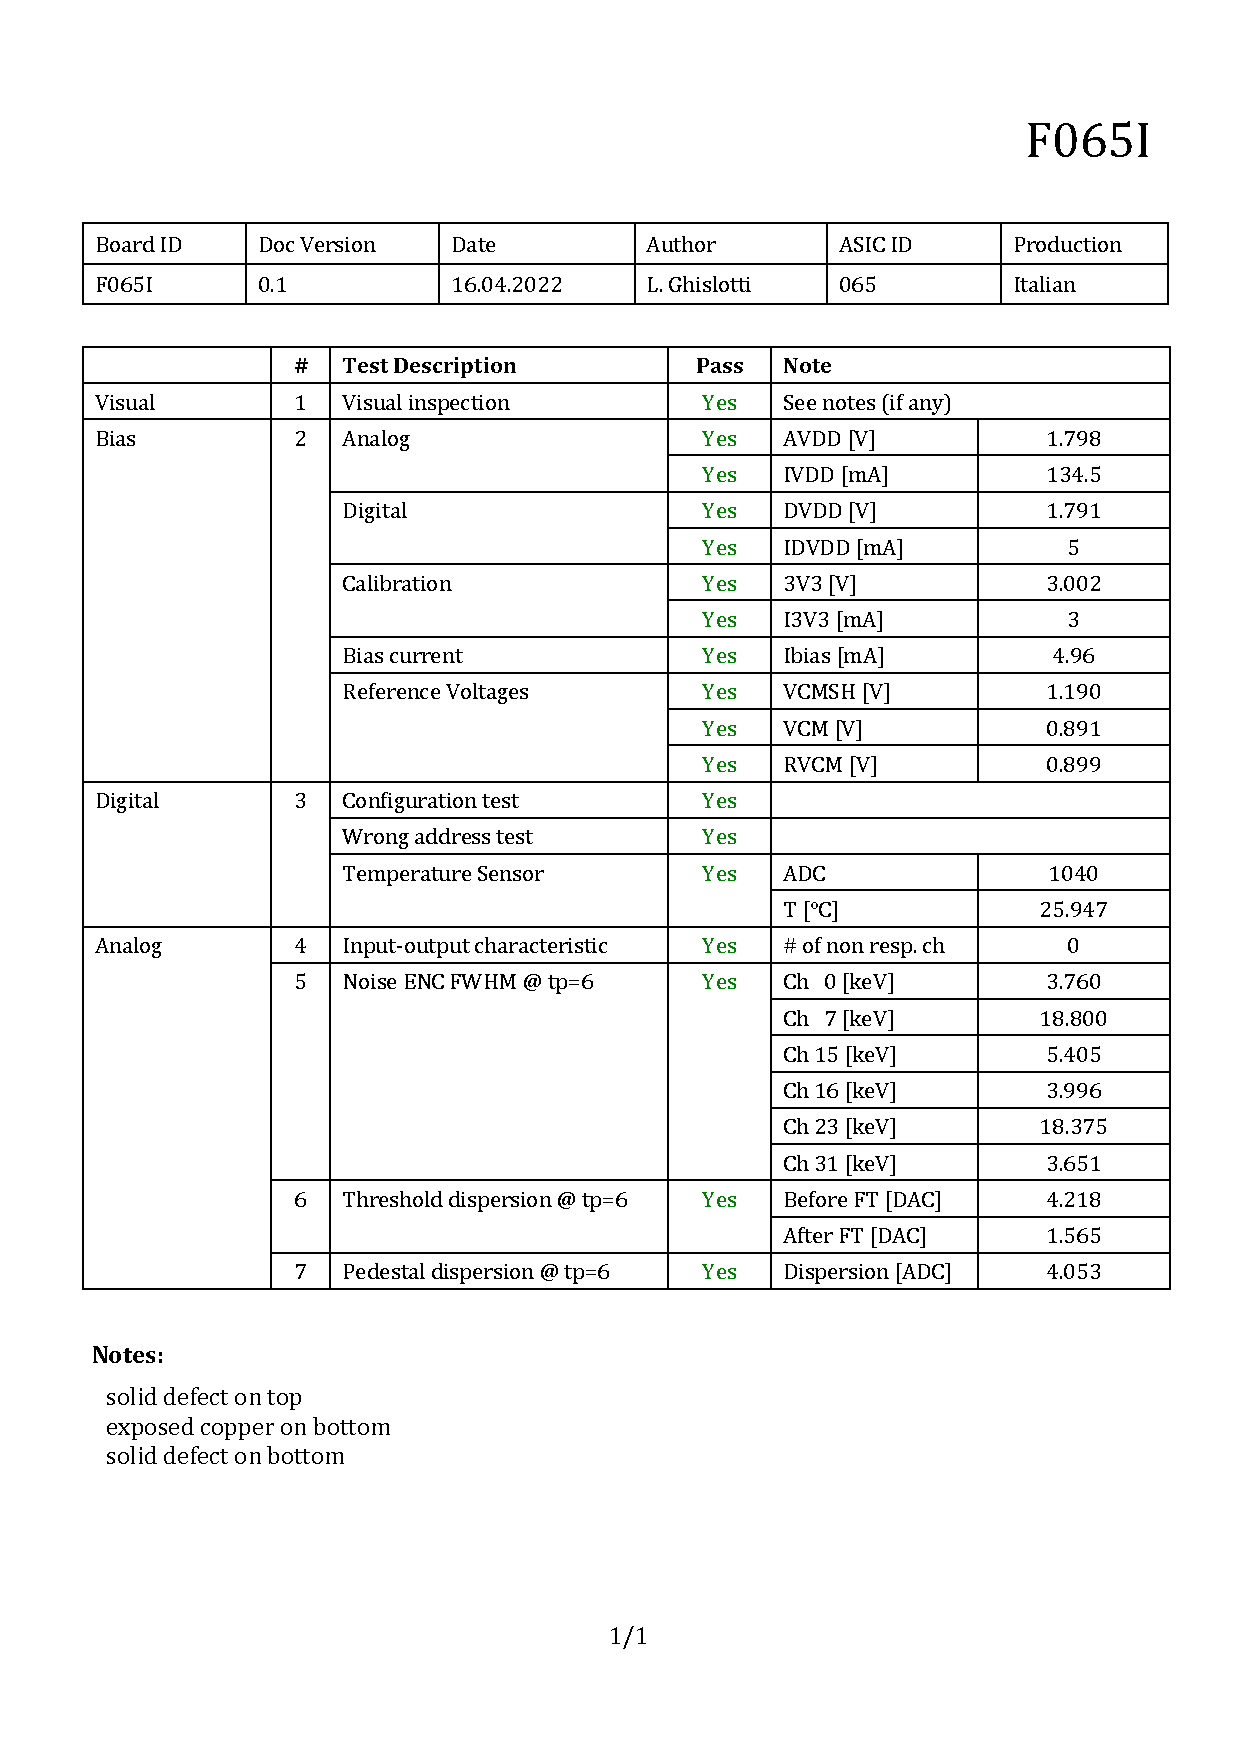
\includegraphics[width=0.5\textwidth]{images/flight_components_validation/F065I.pdf}
            }
    \end{columns}   
\end{frame}


%---------------------------------------------------------------------------------------
%	Experimental results from module test
%---------------------------------------------------------------------------------------

\begin{frame}{Experimental results from module test}
    \settowidth{\leftmargini}{\usebeamertemplate{itemize item}}
    \addtolength{\leftmargini}{\labelsep}
    \fontsize{8.5pt}{1}\selectfont
    \begin{columns}
        \column{0.53\textwidth}
            \vskip0.15cm
            \textbf{\large \textcolor{ForestGreen}{Test setup}}\\
            \vspace{0.1cm}
            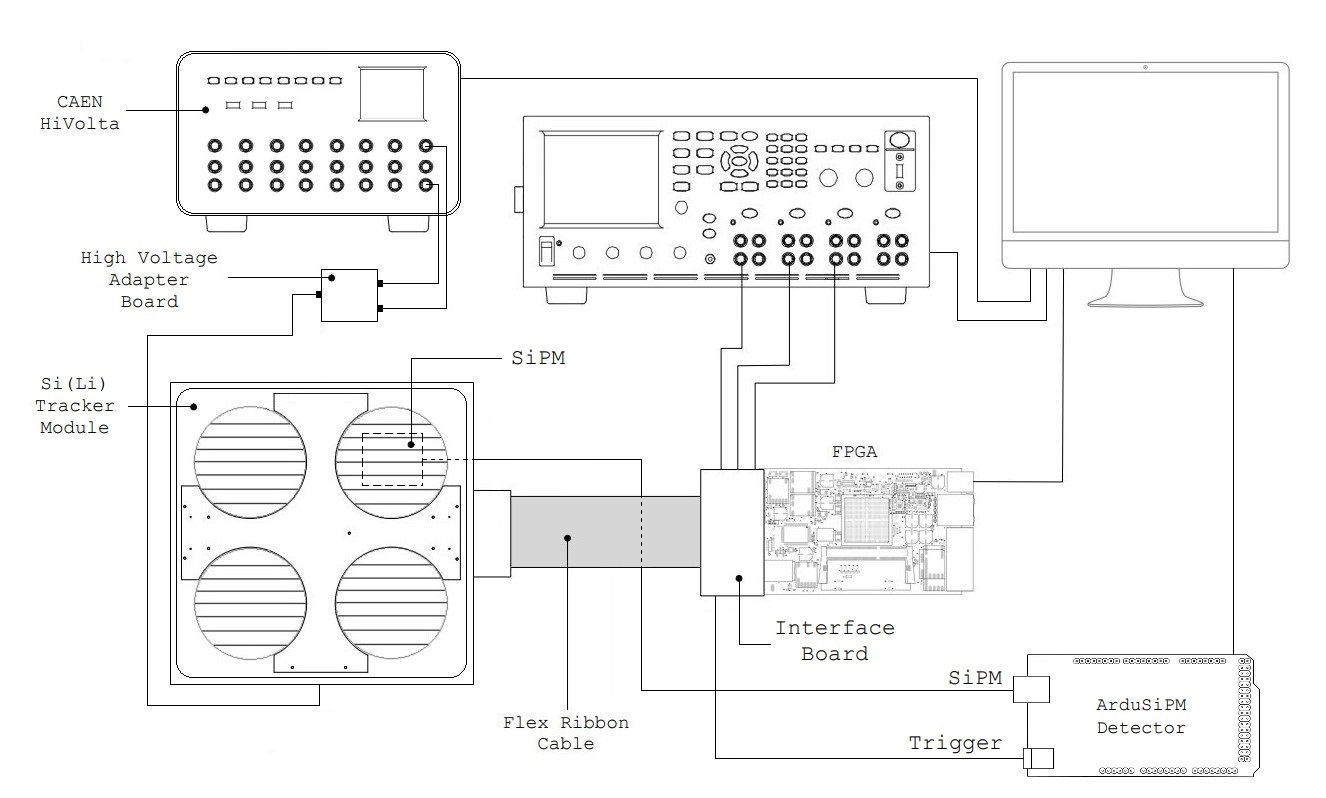
\includegraphics[width=0.95\textwidth]{images/muon_detection/test_setup_MODULE.jpg}
            \vspace{0.15cm}
            \begin{itemize}
                \item Experiment conducted in climate chamber at \textbf{\SI{-40}{\celsius}} and \textbf{\SI{10}{\percent}} relative humidity
                \item Si(Li) detectors biased at \textbf{\SI{-250}{\volt}}
                \item Purposely developed Python script employed to acquire data from readout electronics using an FPGA
                \item Two tests conducted: \textcolor{Red}{\textbf{X-ray}} and \textcolor{Red}{\textbf{muon}} detection
            \end{itemize}
        \column{0.43\textwidth}
            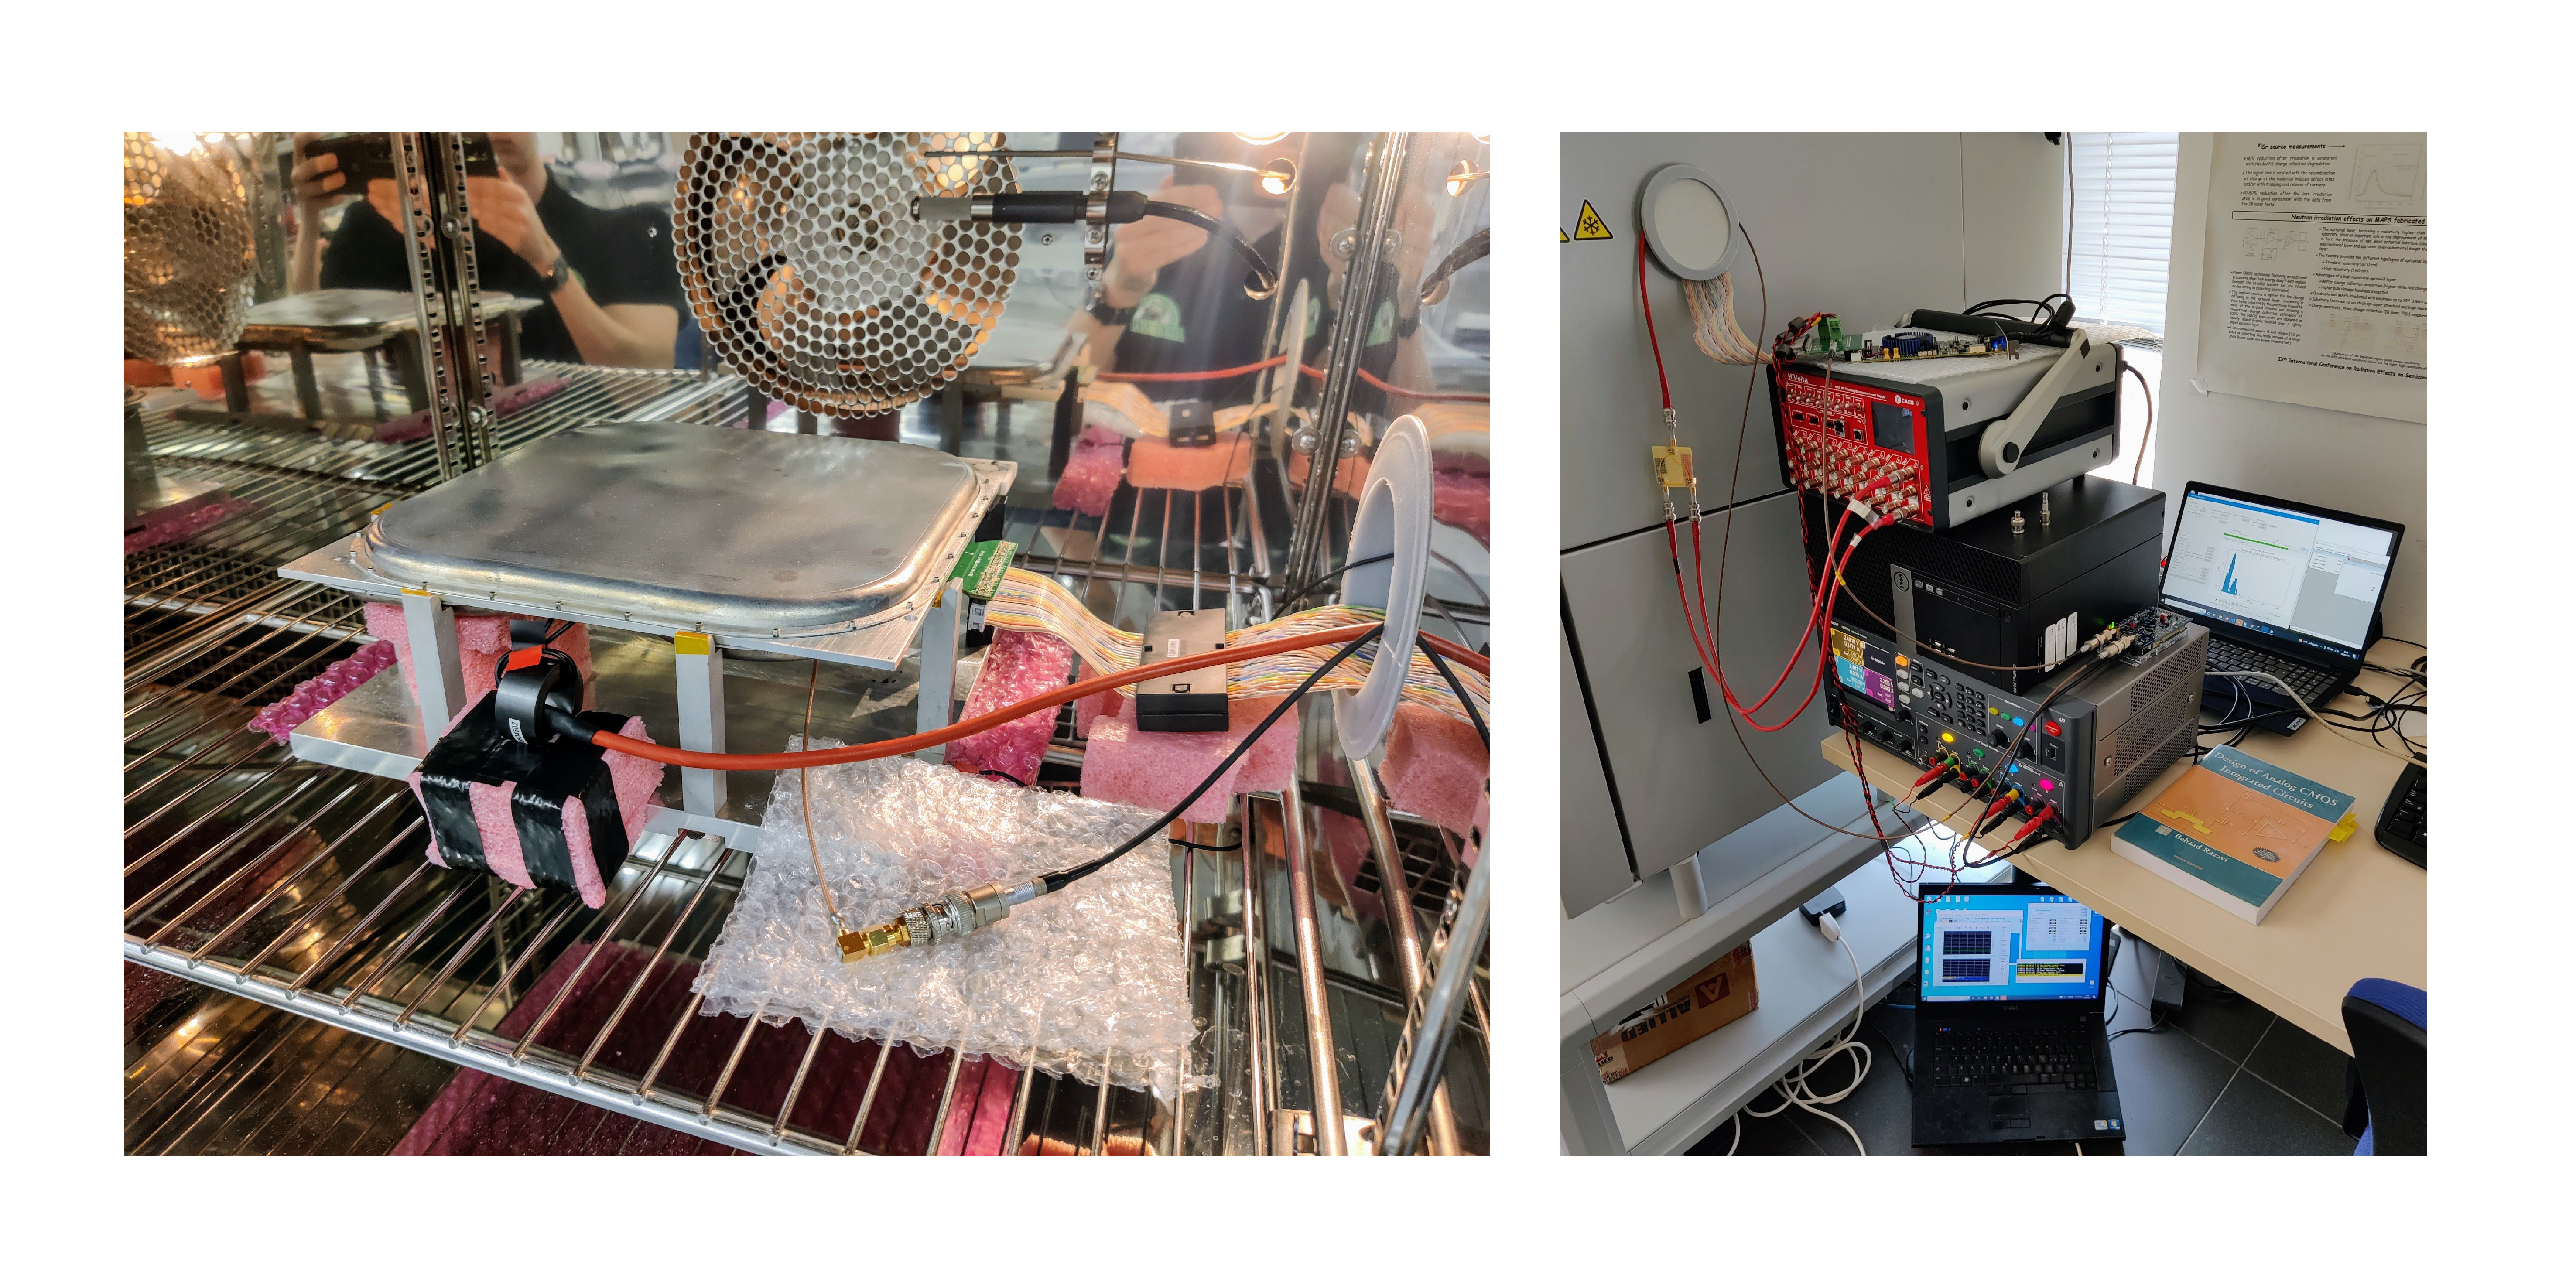
\includegraphics[width=0.97\textwidth]{images/muon_detection/foto_modulo_camera.pdf}
            \vspace{0.2cm}
            \begin{columns}
                \column{0.5\textwidth}
                    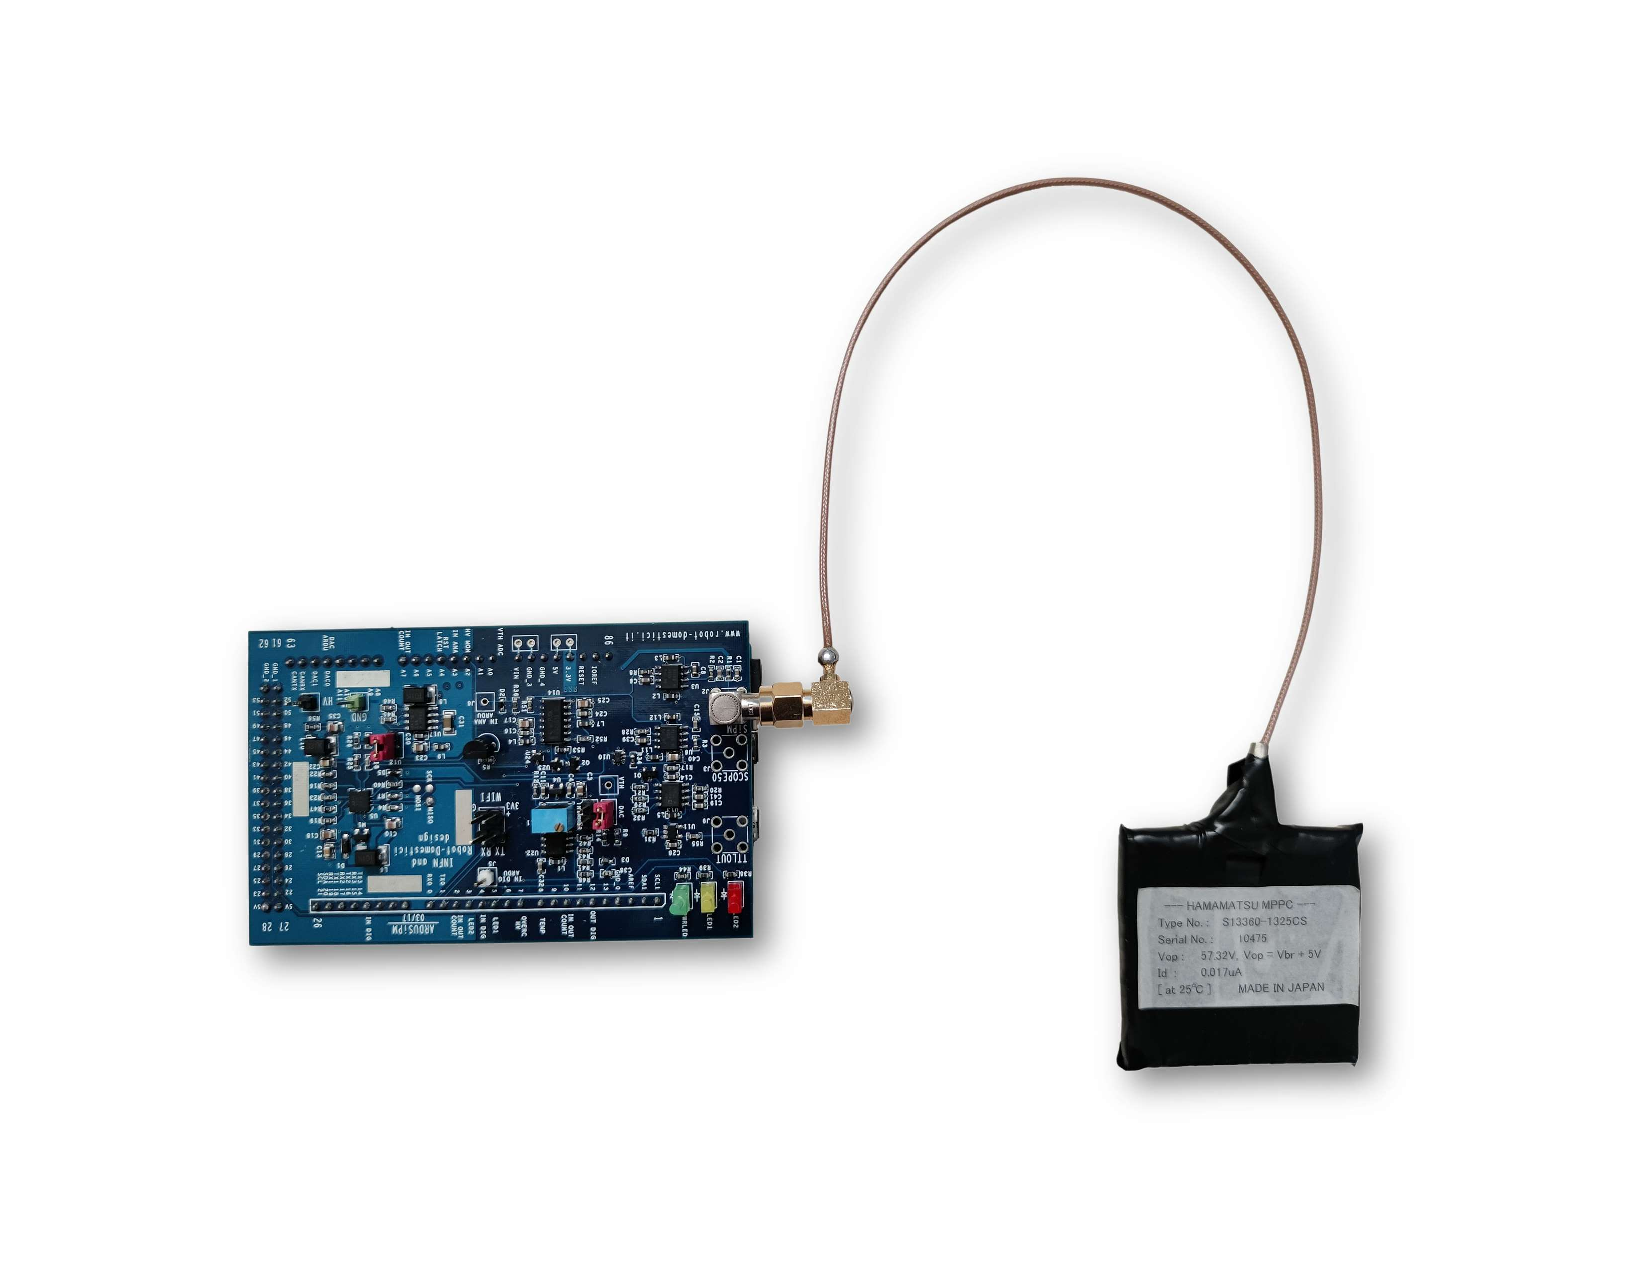
\includegraphics[width=1\textwidth]{images/muon_detection/ardusipm_cropped.pdf}
                \column{0.5\textwidth}
                    \begin{itemize}
                        \item External trigger for\\ cosmic muon detection provided\\ by \textbf{ArduSiPM} radiation detector\vspace{0.1cm}
                        \item Scintillator/SiPM assembly placed underneath one\\ Si(Li) detector
                    \end{itemize}   
            \end{columns}
            \centering
            \vspace{0.3cm}
            \textbf{Americium 241} source placed underneath\\ detector \#0 (Channels 0 to 7) during X-ray detection experiment
    \end{columns}
\end{frame}


%---------------------------------------------------------------------------------------
%	X-ray detection with 241Am source
%---------------------------------------------------------------------------------------

\begin{frame}{X-ray detection with \ce{^{241}Am} source}
    \settowidth{\leftmargini}{\usebeamertemplate{itemize item}}
    \addtolength{\leftmargini}{\labelsep}
    \fontsize{9pt}{1}\selectfont
    \vspace{0.1cm}
    \begin{columns}
        \column{0.65\textwidth}
            \centering
            \textbf{\hspace{0.7cm}Channel 0 to 7: 2 hours acquisition in self-trigger mode}
            \vskip0.1cm
            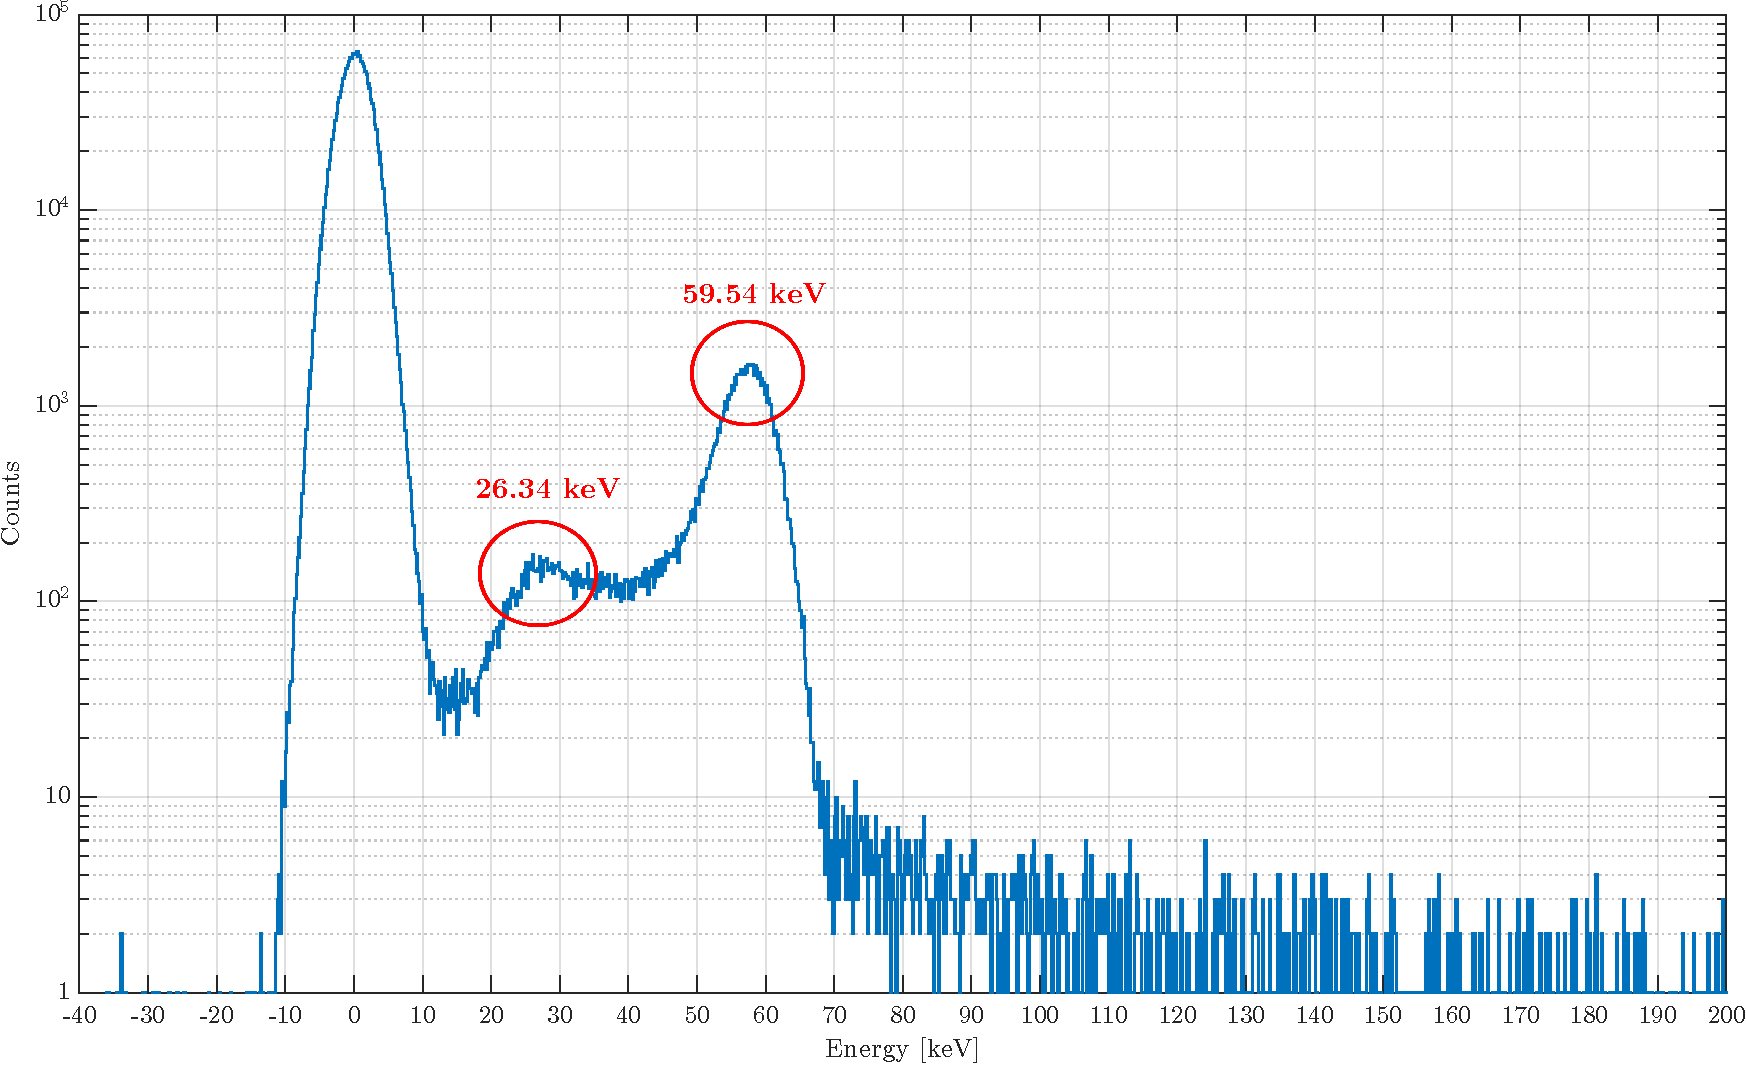
\includegraphics[width=1.06\textwidth]{images/muon_detection/americium/ch4_americio_log.pdf}
        \column{0.3\textwidth}
            \centering
            \fontsize{8.5pt}{1}\selectfont
            \textbf{Channel 6: \SI{10}{\kilo\electronvolt} threshold}
            \vskip0.1cm
            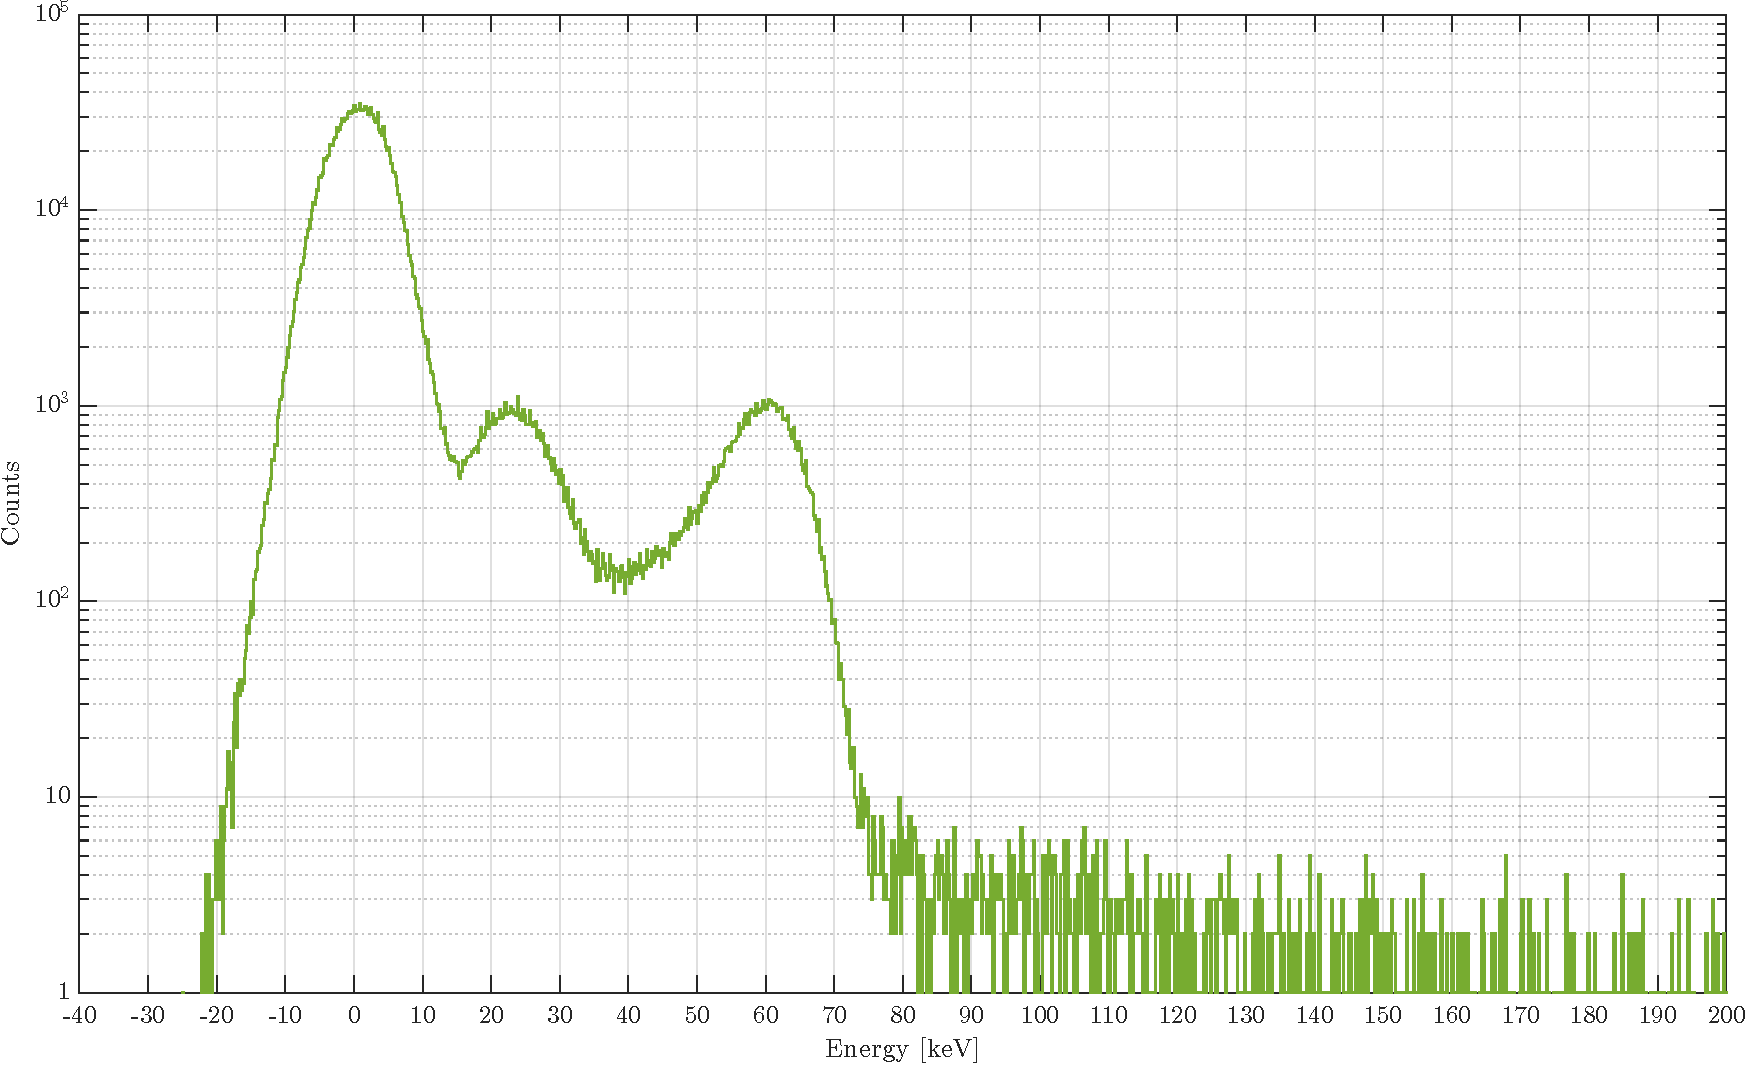
\includegraphics[width=0.99\textwidth]{images/muon_detection/americium/ch4_americio_log_ch6.pdf}
            \vskip0.18cm
            \textbf{Channel 7: \SI{33}{\kilo\electronvolt} threshold}
            \vskip0.1cm
            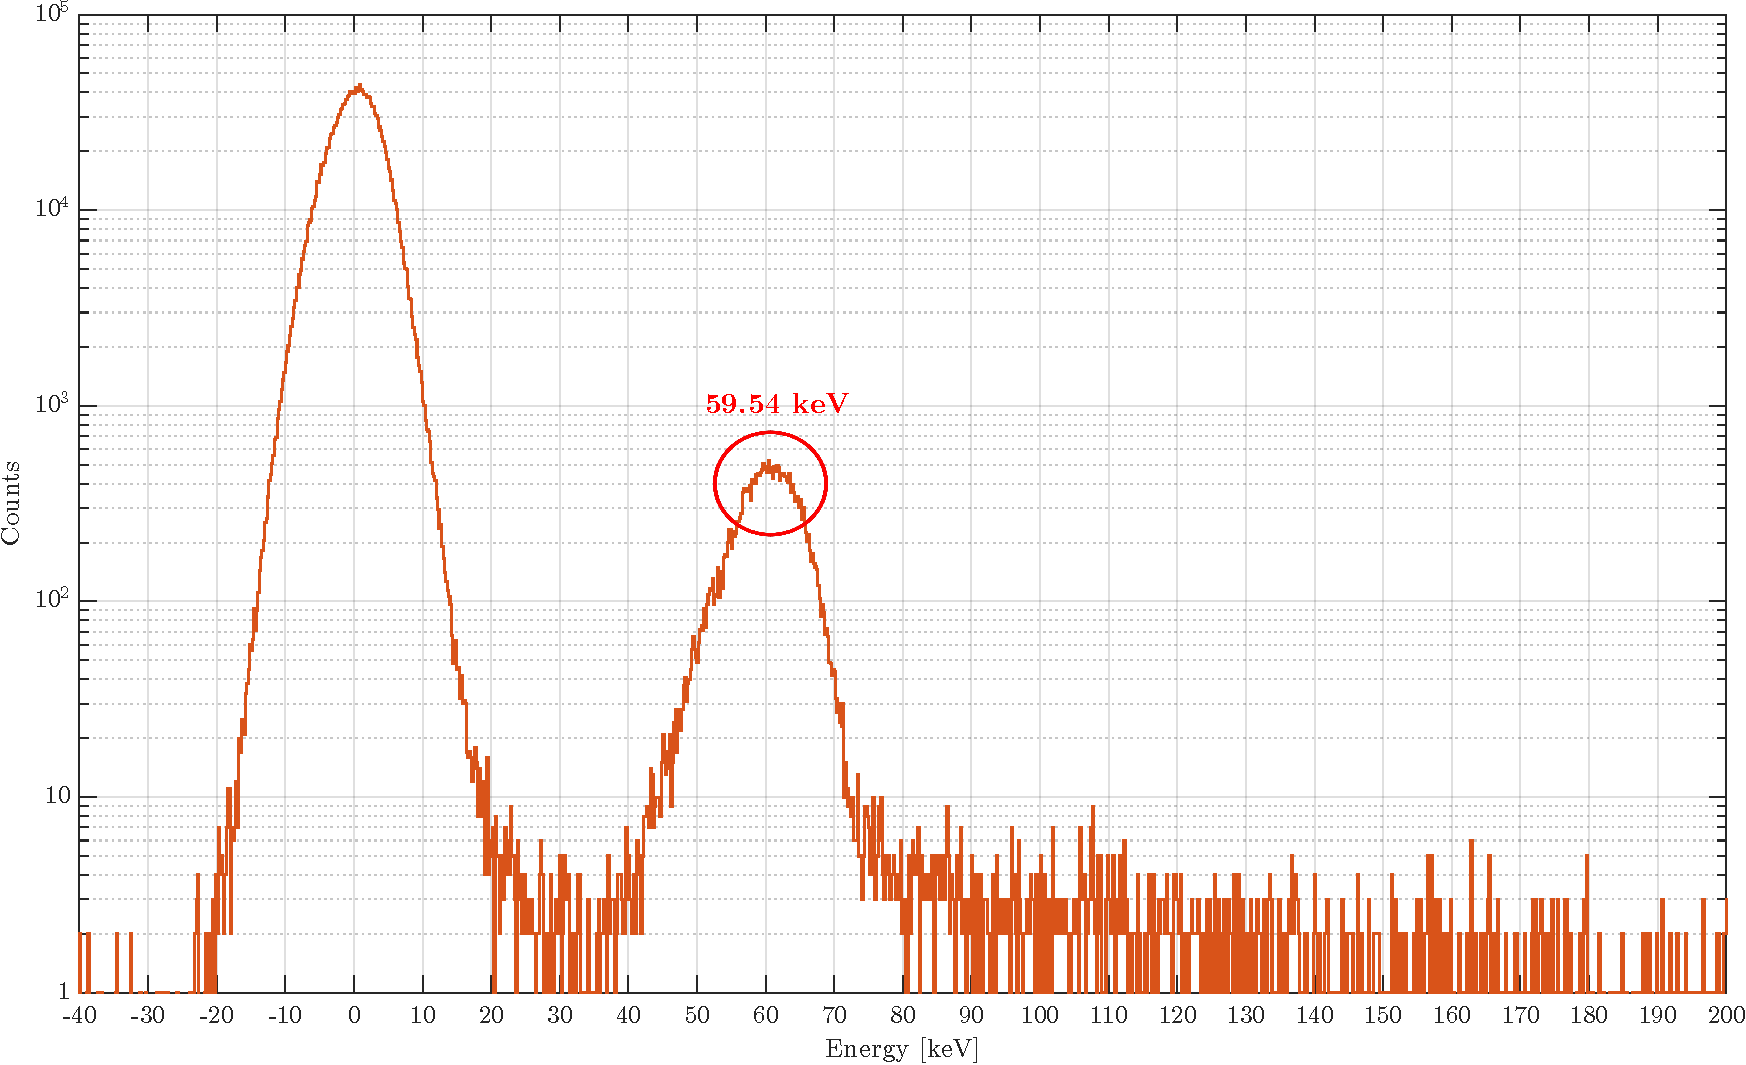
\includegraphics[width=0.99\textwidth]{images/muon_detection/americium/ch4_americio_log_ch7.pdf}  
    \end{columns}
    \fontsize{8.5pt}{1}\selectfont
    \vspace{0.2cm}
    \begin{tabular}{R{3cm} L{6.2cm} L{5cm}}
         \textbf{\textcolor{Red}{Americium 241 source:}} & radioactive isotope with 432.2 years half-life & $\rightarrow$ \hspace{0.2cm} both peaks detected \greencheck \B \\
         & emits X-ray radiation at \textbf{\SI{59.54}{\kilo\electronvolt}} and \textbf{\SI{26.34}{\kilo\electronvolt}}
    \end{tabular}
\end{frame}


%---------------------------------------------------------------------------------------
%	Cosmic muon detection in self trigger mode
%---------------------------------------------------------------------------------------

\begin{frame}{Cosmic muon detection in self trigger mode}
    %\settowidth{\leftmargini}{\usebeamertemplate{itemize item}}
    %\addtolength{\leftmargini}{\labelsep}

    \begin{columns}[T]
        \column{0.5\textwidth}
            \centering
            \fontsize{9pt}{1}\selectfont
            \vskip-0.1cm
            \textbf{Self trigger mode\\ with and without zero suppression}
            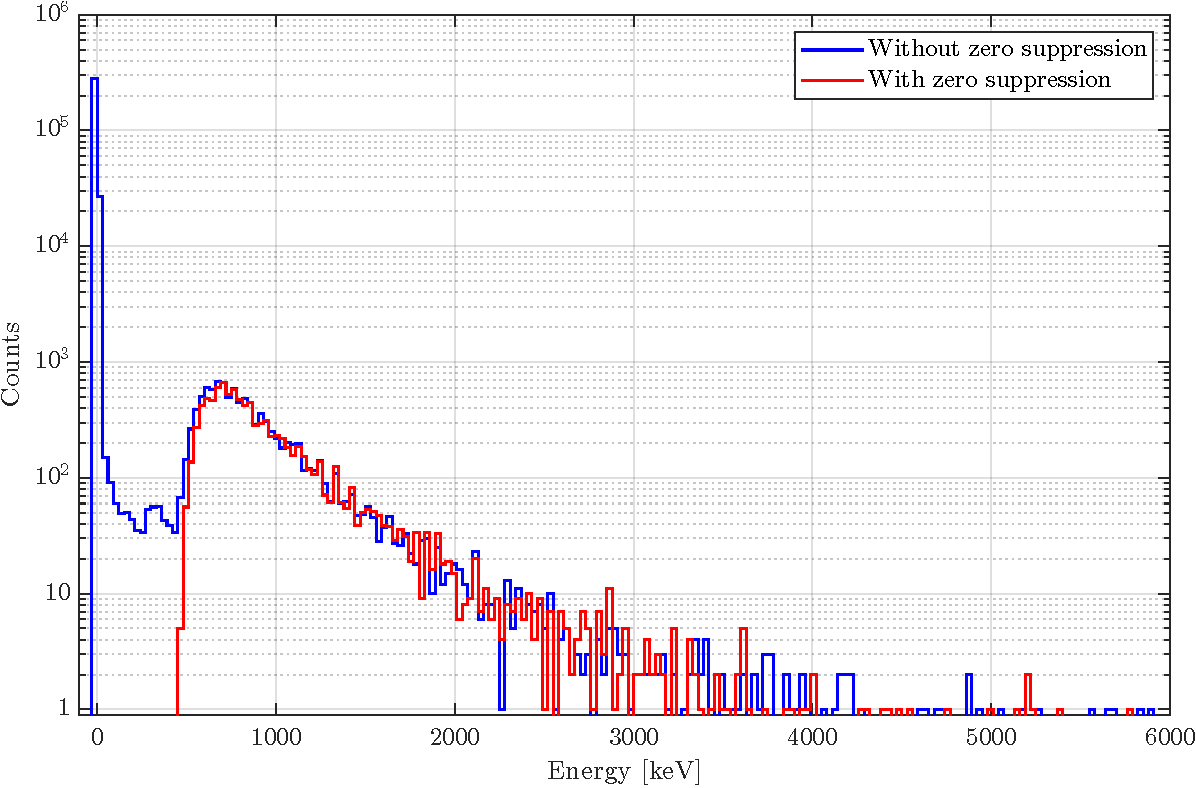
\includegraphics[width=0.9\textwidth]{images/muon_detection/incoming_energy_zero_suppr_thr130_keV.pdf}

            \fontsize{8.5pt}{1}\selectfont
            \vspace{0.1cm}
            \begin{itemize}
                \item \textbf{Zero suppression}: channel output sampled by ADC only if signal over threshold comparator fires
                \item 32 channels readout for 1 hour
                \item Threshold set to \textbf{\SI{450}{\kilo\electronvolt}}
            \end{itemize}

            \begin{textblock*}{\textwidth}(0.7cm, 8.1cm)
                \fontsize{6pt}{1}\selectfont
                \raggedright
                \textcolor{Black}{(*) F. Rogers et al., “Large-area Si(Li) detectors for X-ray spectrometry and particle tracking in the GAPS experiment” Journal of Instrumentation, vol. 14, Art. no. 10, 2019, doi: 10.1088/1748-0221/14/10/p10009}
            \end{textblock*}

        \column{0.5\textwidth}
            \centering
            \fontsize{9pt}{1}\selectfont
            \vskip-0.1cm
            \textbf{Landau distribution\\ in zero suppression mode}
            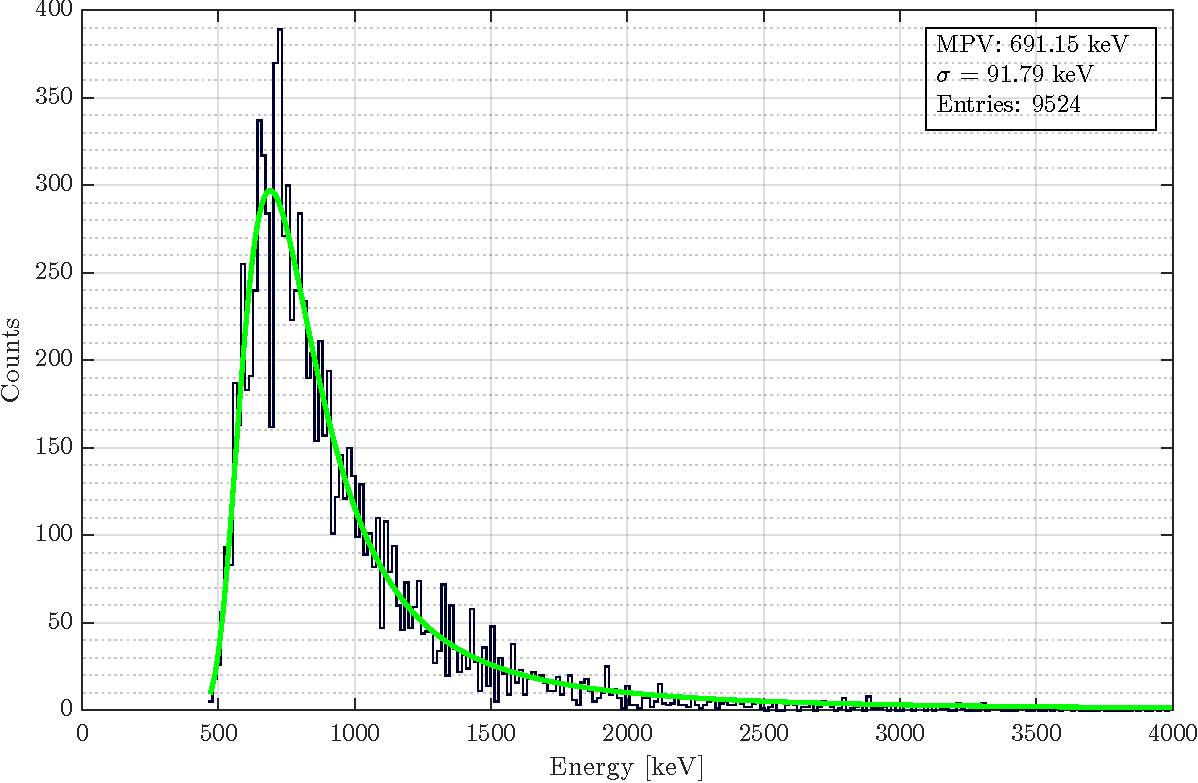
\includegraphics[width=0.9\textwidth]{images/muon_detection/incoming_energy_thr130_ZS_landau_keV.pdf}

             \fontsize{8.5pt}{1}\selectfont
            \vspace{0.1cm}
            \begin{itemize}
                \item Data acquisition performed in zero suppression mode
                \item Data fitted with \textbf{Landau distribution}
                \item Most probable value peaked in \textbf{$\approx \SI{691}{\kilo\electronvolt}$} \greencheck
                \item Measurement is consistent with data acquired with the same type of Si(Li) detector and discrete electronics (*) \greencheck
            \end{itemize}
    \end{columns}
\end{frame}


%---------------------------------------------------------------------------------------
%	Cosmic muon detection with external scintillator
%---------------------------------------------------------------------------------------

\begin{frame}{Cosmic muon detection with external scintillator}
    \settowidth{\leftmargini}{\usebeamertemplate{itemize item}}
    \addtolength{\leftmargini}{\labelsep}
    \fontsize{9pt}{1}\selectfont
    \begin{columns}
        \column{0.34\textwidth}
        \begin{itemize}
            \item Scintillator/SiPM assembly placed underneath Si(Li) detector \#2: channels 16 to 23 highlighted in red
            \vskip0.4cm
            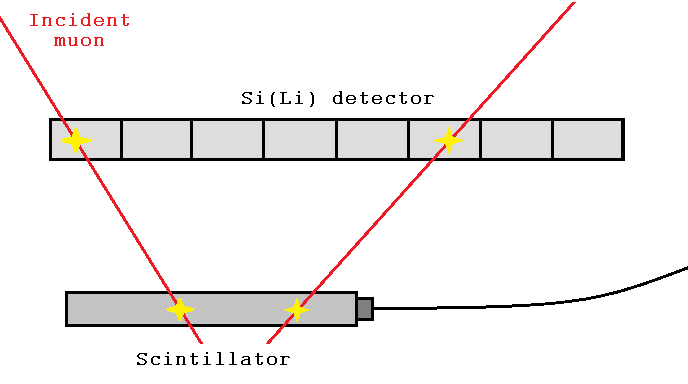
\includegraphics[width=0.9\textwidth]{images/muon_detection/scintillator_sensor_detail.png}
            \vskip0.4cm
            \item \textbf{ArduSiPM} radiation detector used as an external trigger source
            \item 2 hours acquisition
            \item Global threshold set to \textbf{\SI{450}{\kilo\electronvolt}}
            \item Peaking time \#4 ($\tau_{p} = \SI{980}{\nano\second}$)
            \item Trigger hold delay set to \texttt{34} FPGA clocks ($\approx \SI{708}{\nano\second}$)
        \end{itemize}
        \column{0.6\textwidth}
            \vskip-0.2cm
            \begin{figure}[h!]
                \centering
                \begin{tabular}{c c}
                    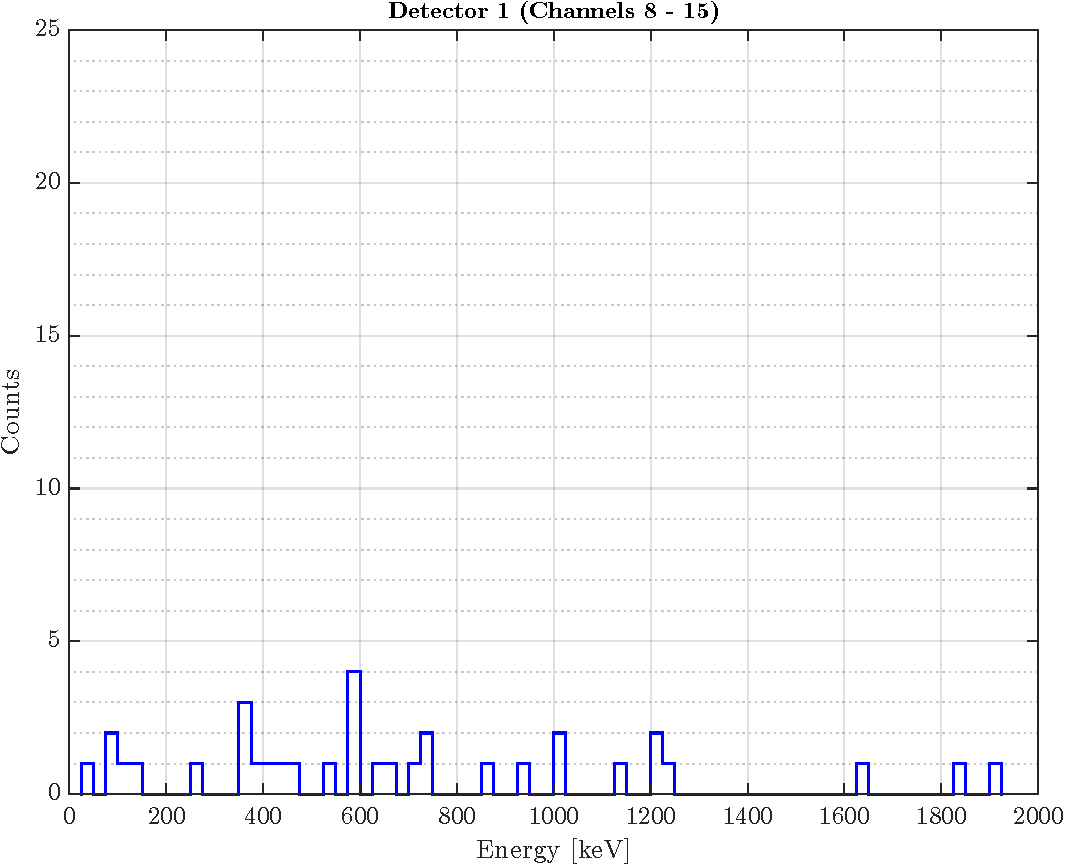
\includegraphics[width=0.47\textwidth]{images/muon_detection/incoming_energy34_2hr_sens2_keV_lin.pdf} & 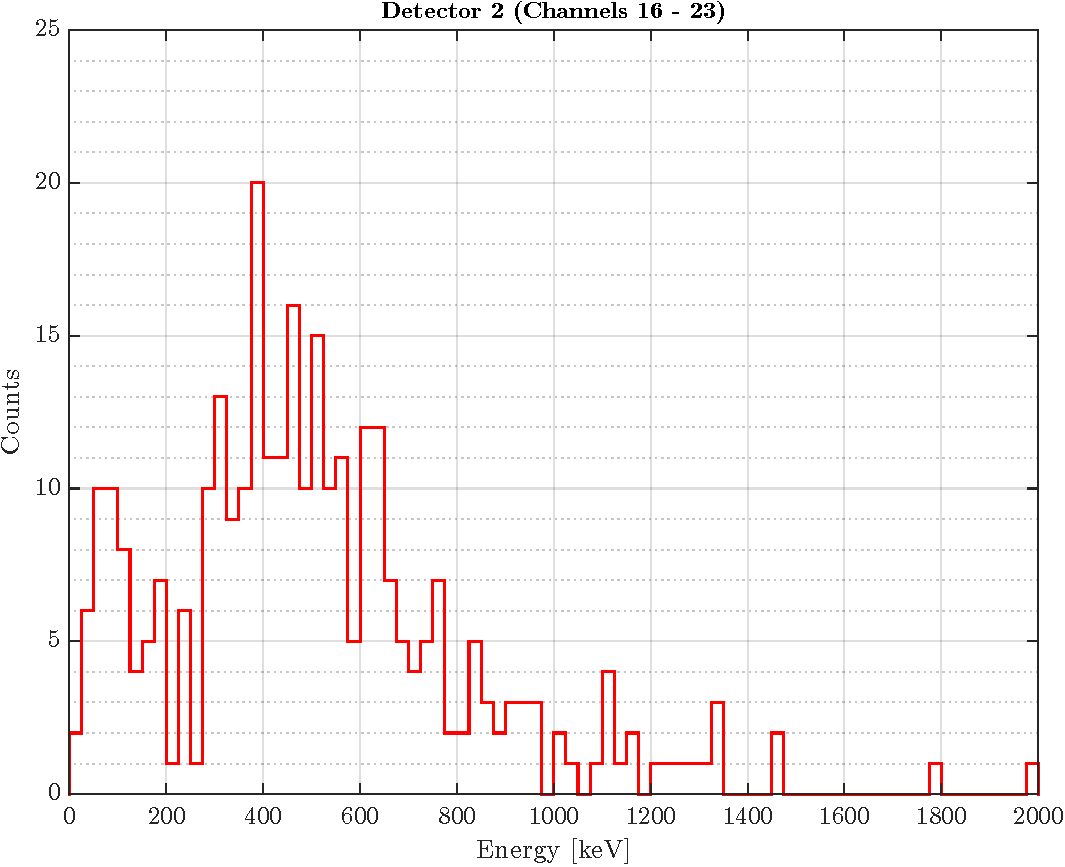
\includegraphics[width=0.47\textwidth]{images/muon_detection/incoming_energy34_2hr_sens3_keV_lin.pdf}\B \\
                    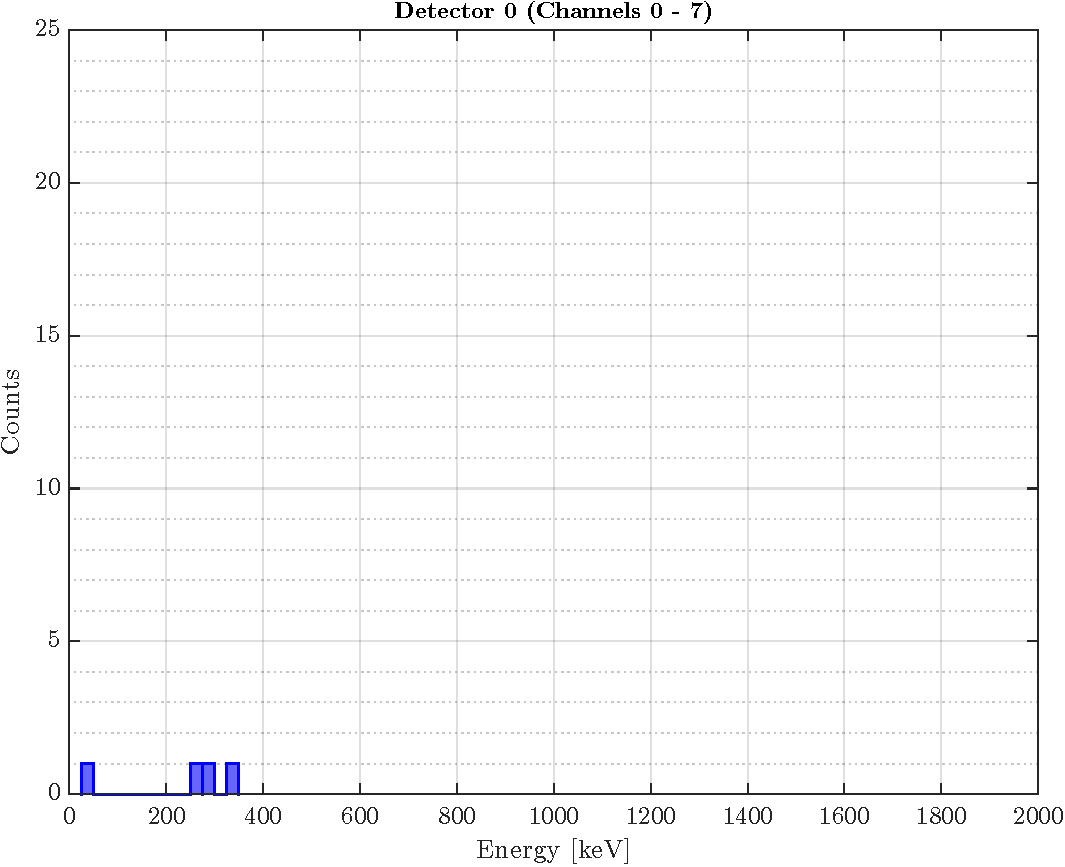
\includegraphics[width=0.47\textwidth]{images/muon_detection/incoming_energy34_2hr_sens1_keV_lin.pdf} & 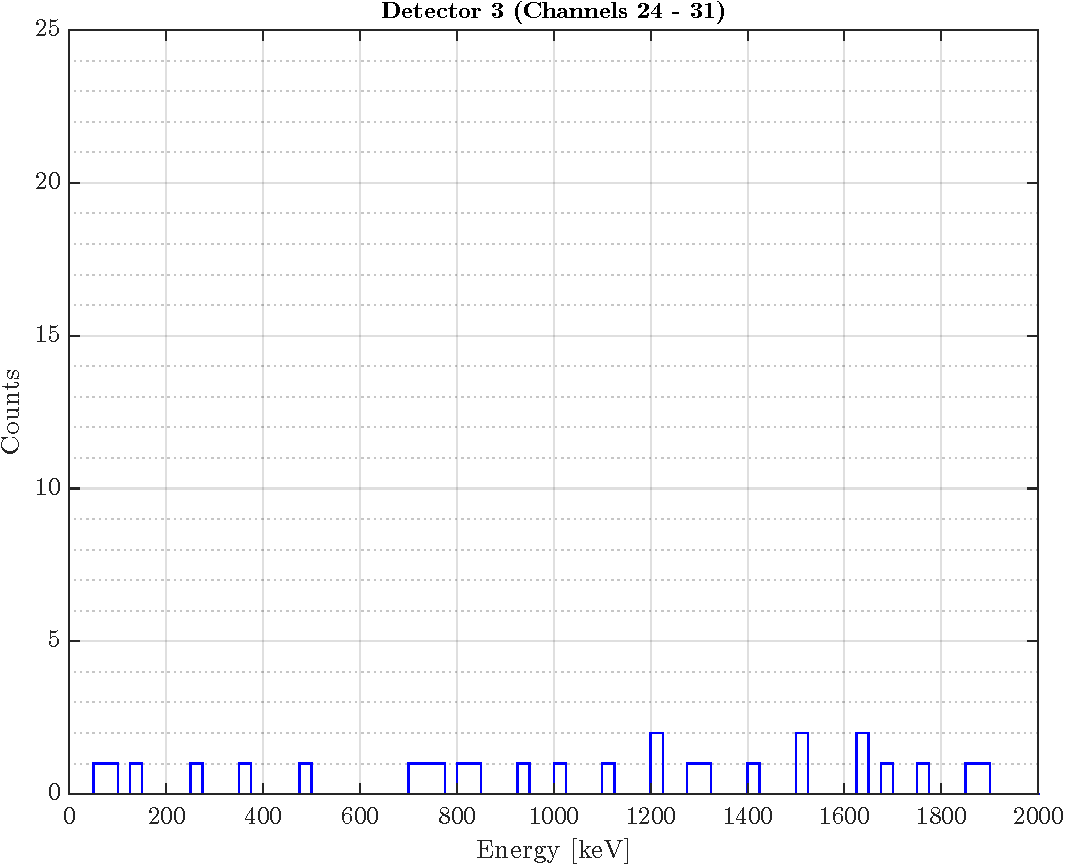
\includegraphics[width=0.47\textwidth]{images/muon_detection/incoming_energy34_2hr_sens4_keV_lin.pdf}
                \end{tabular}
            \end{figure}
    \end{columns}
\end{frame}


%---------------------------------------------------------------------------------------
%	Conclusions
%---------------------------------------------------------------------------------------

\begin{frame}{Conclusions and next steps}
    \begin{columns}
        \column{0.96\textwidth}
            \fontsize{11pt}{1}\selectfont
            \pause
            \textbf{Conclusions}
            \vspace{0.16cm}
            \fontsize{10pt}{1}\selectfont
            \begin{enumerate}
                \setlength\itemsep{0.5em}
                \item Readout electronics performing as expected under different temperature conditions and design requirements are met \pause
                \item All flight items have been successfully tested and shipped to Columbia University for final assembly \pause
                \item Demonstrated ability to detect cosmic muons and X-rays above \SI{20}{\kilo\electronvolt} with promising results \pause
            \end{enumerate}
        
            \vspace{0.4cm}
            \fontsize{11pt}{1}\selectfont
            \textbf{Next steps}
            \vspace{0.16cm}
            \fontsize{10pt}{1}\selectfont
            \begin{itemize}
                \setlength\itemsep{0.5em}
                \item Final assembly is ongoing at the Space Sciences Laboratory in Berkeley, California \pause
                \item Thermal Vacuum Chamber test to be performed in \textbf{April 2023} at the NASA’s Neil Armstrong Test Facility in Cleveland, Ohio \pause
                \item Pre-flight instrument setup at the Columbia Scientific Balloon Facility in Palestine, Texas in \textbf{August 2023} \pause
                \item First flight from the National Science Foundation McMurdo station in Antarctica in \textbf{December 2023}
            \end{itemize}
            
    \end{columns}
\end{frame}


%---------------------------------------------------------------------------------------
%	Last picture
%---------------------------------------------------------------------------------------

\appendix
\backupbegin

\begin{frame}[plain,noframenumbering]
    \centering
    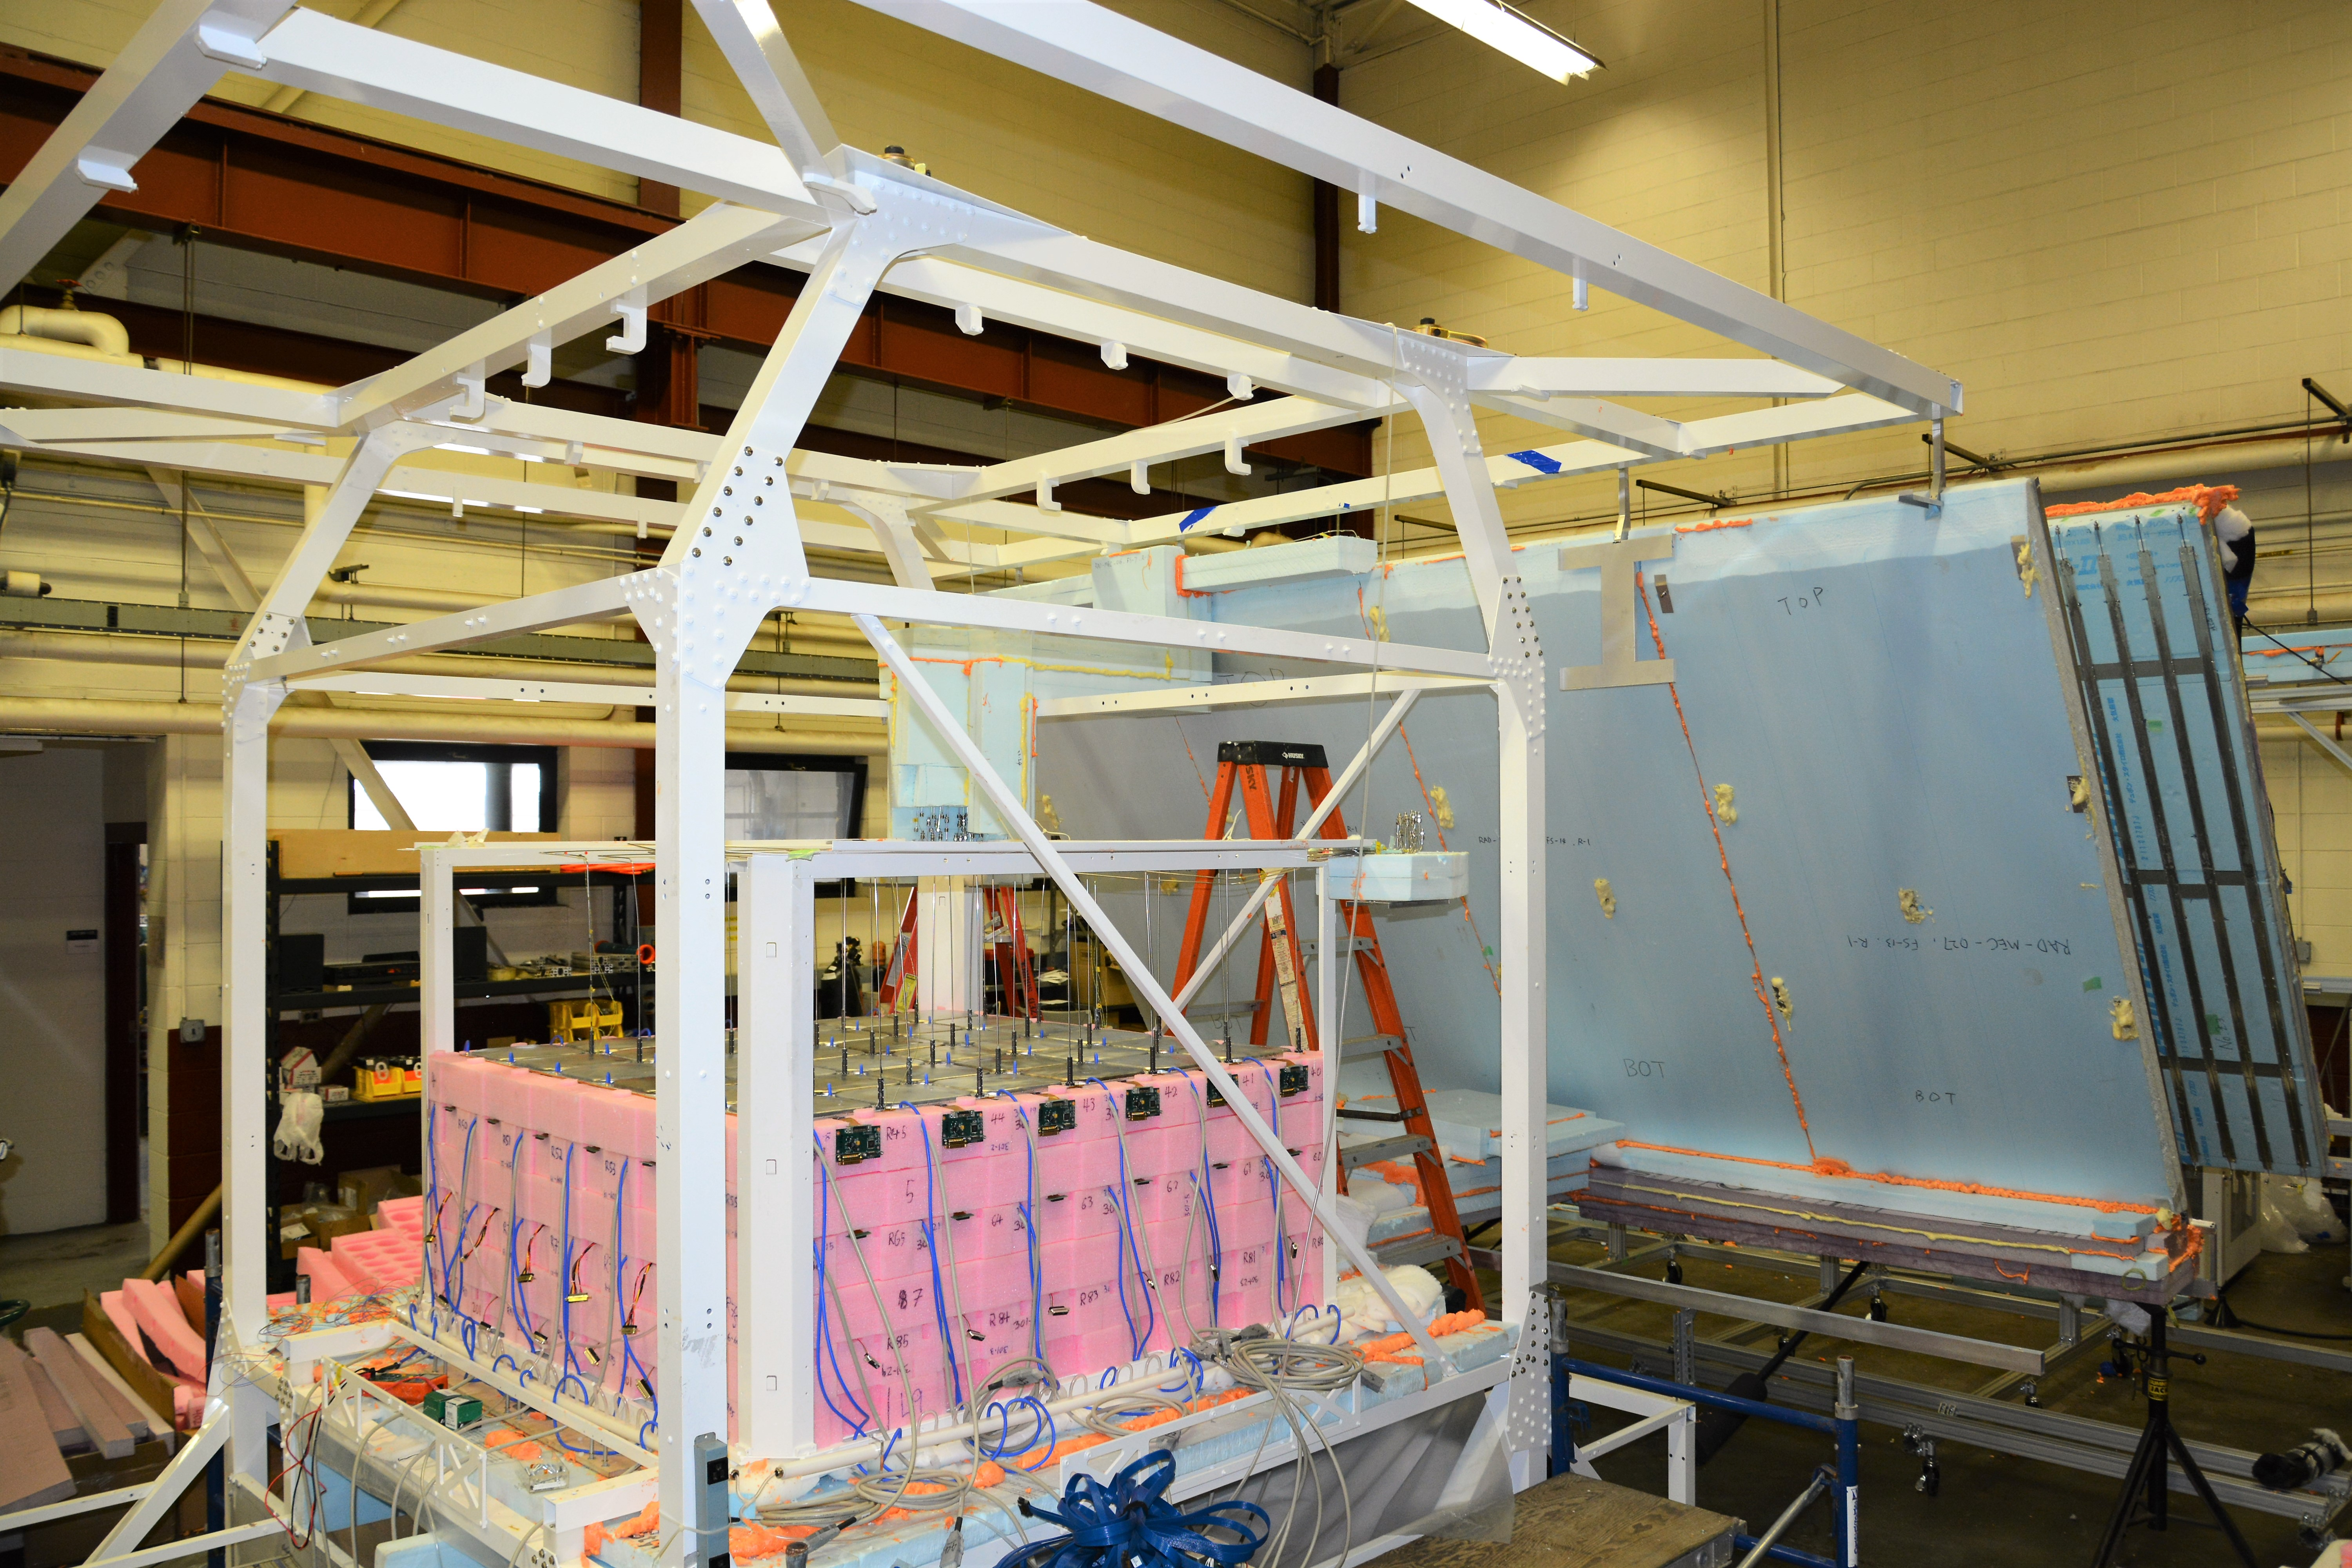
\includegraphics[width=0.8\textwidth]{images/random/immagine_finale_menjiao.jpg}
\end{frame}


%---------------------------------------------------------------------------------------
%	Backup slides
%---------------------------------------------------------------------------------------

\begin{frame}[plain,noframenumbering]{}
    \fontsize{20pt}{1}\selectfont
    \centering
    \vspace{1.5cm}
    \textbf{Backup slides}
\end{frame}


%---------------------------------------------------------------------------------------
%	Analog readout channel and ADC
%---------------------------------------------------------------------------------------

\begin{frame}{Analog readout channel and ADC}
    \fontsize{8.5pt}{1}\selectfont
    \settowidth{\leftmargini}{\usebeamertemplate{itemize item}}
    \addtolength{\leftmargini}{\labelsep}
    \centering
    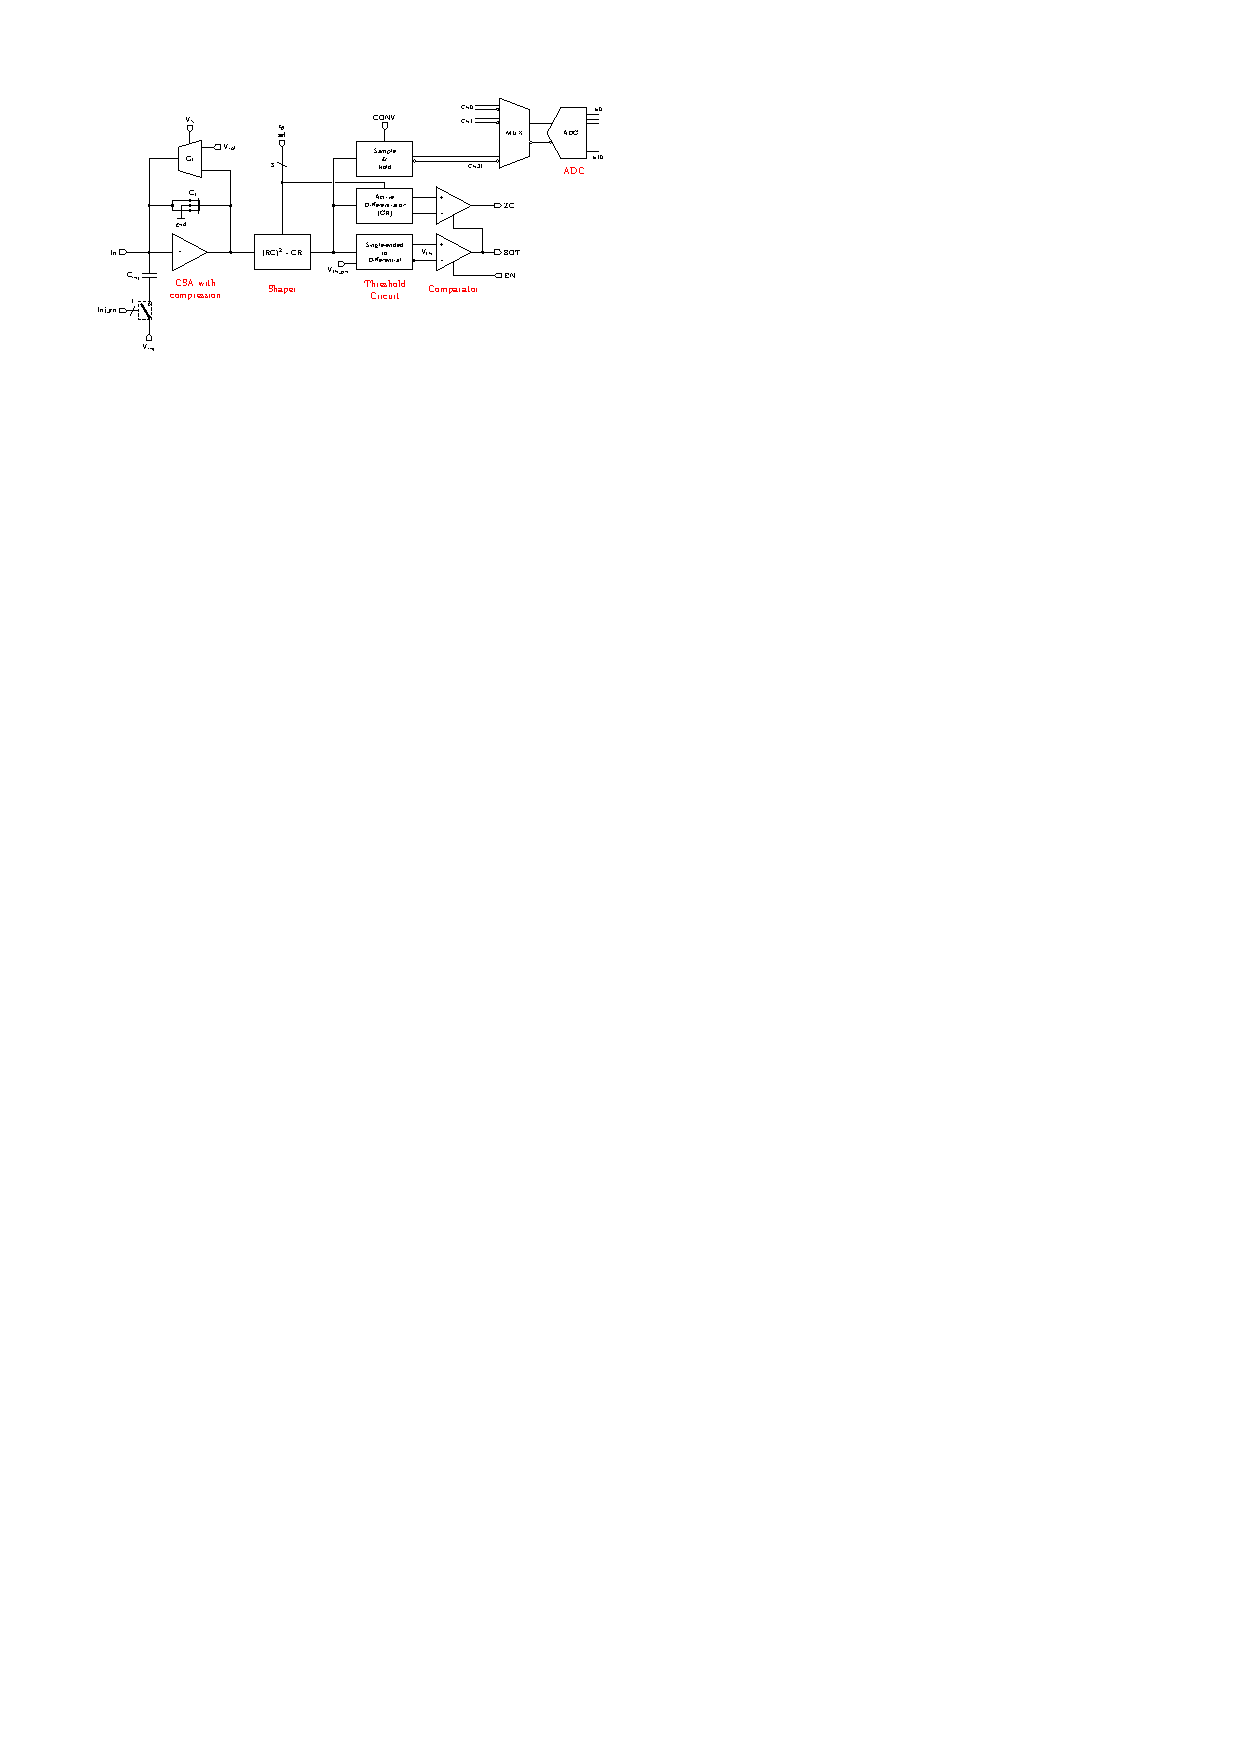
\includegraphics[width=0.68\textwidth]{images/backup_slides/readoutchannelADC.pdf}
    \vskip0.2cm
    \begin{columns}[T]
        \column{0.3\textwidth}
            \begin{itemize}
                \item \textbf{Charge Sensitive Amplifier}\\ with dynamic signal compression
                \item \textbf{CR-(RC)$^{2}$ filter}\\ with 8 selectable peaking times (from \SI{250}{\nano\second} to \SI{1.8}{\micro\second})
            \end{itemize}
            
        \column{0.36\textwidth}
            \begin{itemize}
                \item \textbf{SOT comparator}\\ Signal Over Threshold identification
                \item \textbf{Active CR and ZC comparator}\\ Shaper signal peak detection
                \item \textbf{Single-ended to differential S\&H}\\ Shaper signal peak storage
            \end{itemize}
        
        \column{0.25\textwidth}
            \begin{itemize}
                \item \textbf{Injection capacitance $C_{inj}$}\\ Used for calibration
                \item \textbf{11-bit hybrid SAR ADC} \\ One per ASIC with 32:1 multiplexer
            \end{itemize}
    \end{columns}
\end{frame}


%---------------------------------------------------------------------------------------
%	SLIDER32 ASIC
%---------------------------------------------------------------------------------------

\begin{frame}{SLIDER32 ASIC}
   \begin{columns}
    \column{0.55\textwidth}
        \vskip0.1cm
        \fontsize{10pt}{1}\selectfont
        \textbf{\textcolor{ForestGreen}{Flight ASIC - CMOS \SI{180}{\nano\meter} technology}}\\
        \vspace{0.3cm}
        \fontsize{9.5pt}{1}\selectfont
        \textbf{\textcolor{Red}{ASIC features}}
        \vspace{0.1cm}
        \begin{itemize}
            \fontsize{9pt}{1}\selectfont
            \setlength\itemsep{0.3em}
            \item 32 analog readout channels
            \item 11-bit ADC
            \item Digital back end (registers control, SPI, ...)
            \item BGR with 3-bit DAC regulation
            \item 8-bit DAC for global threshold setting
            \item 3-bit DAC for threshold fine trimming
            \item Detector leakage current readout
            \item Temperature sensor readout
        \end{itemize}
        \vspace{0.2cm}
        \textbf{\textcolor{Red}{Package}}
        \vspace{0.1cm}
        \begin{itemize}
            \fontsize{9pt}{1}\selectfont
            \setlength\itemsep{0.3em}
            \item Plastic Thin Quad Flat Pack (TQFP128) \vspace{-0.1cm}
            \item $14 \times \SI{14}{\milli\metre\squared}$
            \item 128 pins
            \item Pitch of \SI{0.4}{\milli\metre}
            \item 600 samples fabricated
        \end{itemize}
        
    \column{0.35\textwidth}
        \begin{figure}
        \centering
        \vspace{-0.25cm}
        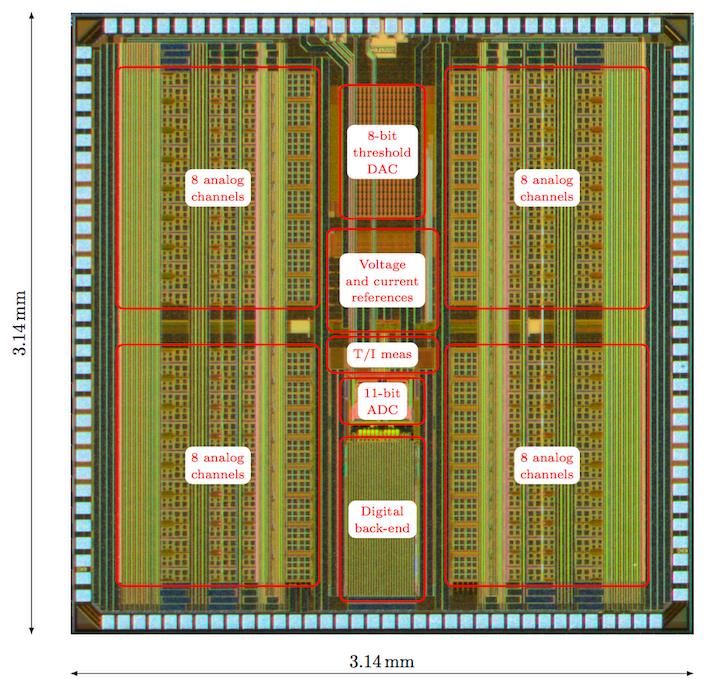
\includegraphics[height=0.5\textheight]{images/experiment_intro/gaps_asic_circuit.jpg}
        \vspace{0.3cm}
        \vskip0.1cm
        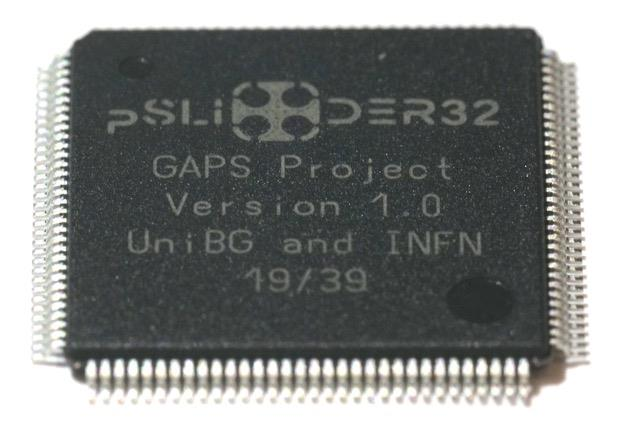
\includegraphics[height=0.22\textheight]{images/backup_slides/SLIDER32_asic_package.jpg}
        \end{figure}
    \end{columns}
\end{frame}


%---------------------------------------------------------------------------------------
%	Dynamic Signal Compression
%---------------------------------------------------------------------------------------

\begin{frame}{Dynamic Signal Compression}
    \fontsize{8.5pt}{1}\selectfont
    \settowidth{\leftmargini}{\usebeamertemplate{itemize item}}
    \addtolength{\leftmargini}{\labelsep}
    \begin{columns}
        \column{0.5\textwidth}
            \begin{itemize}
                \item \textbf{Basic Idea}: exploit the non-linear feature of MOS capacitors to change the gain of CSA with the input signal amplitude
                \item It is based on the nonlinear behaviour of a MOSFET capacitor operating in the inversion mode
                \item Suitable choice of \texttt{W} and \texttt{L} to set the gain in the low and high energy regime 
            \end{itemize}
            \centering
            \vspace{0.5cm}
            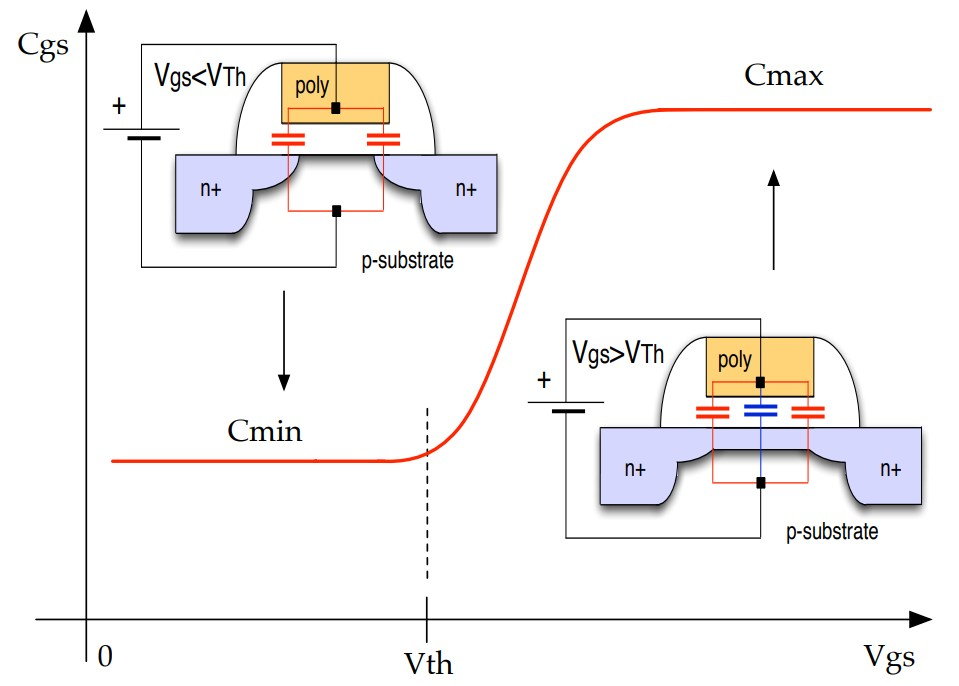
\includegraphics[height=0.5\textheight]{images/backup_slides/capacitance_value_plot.jpg}
        \column{0.5\textwidth}
            \centering
            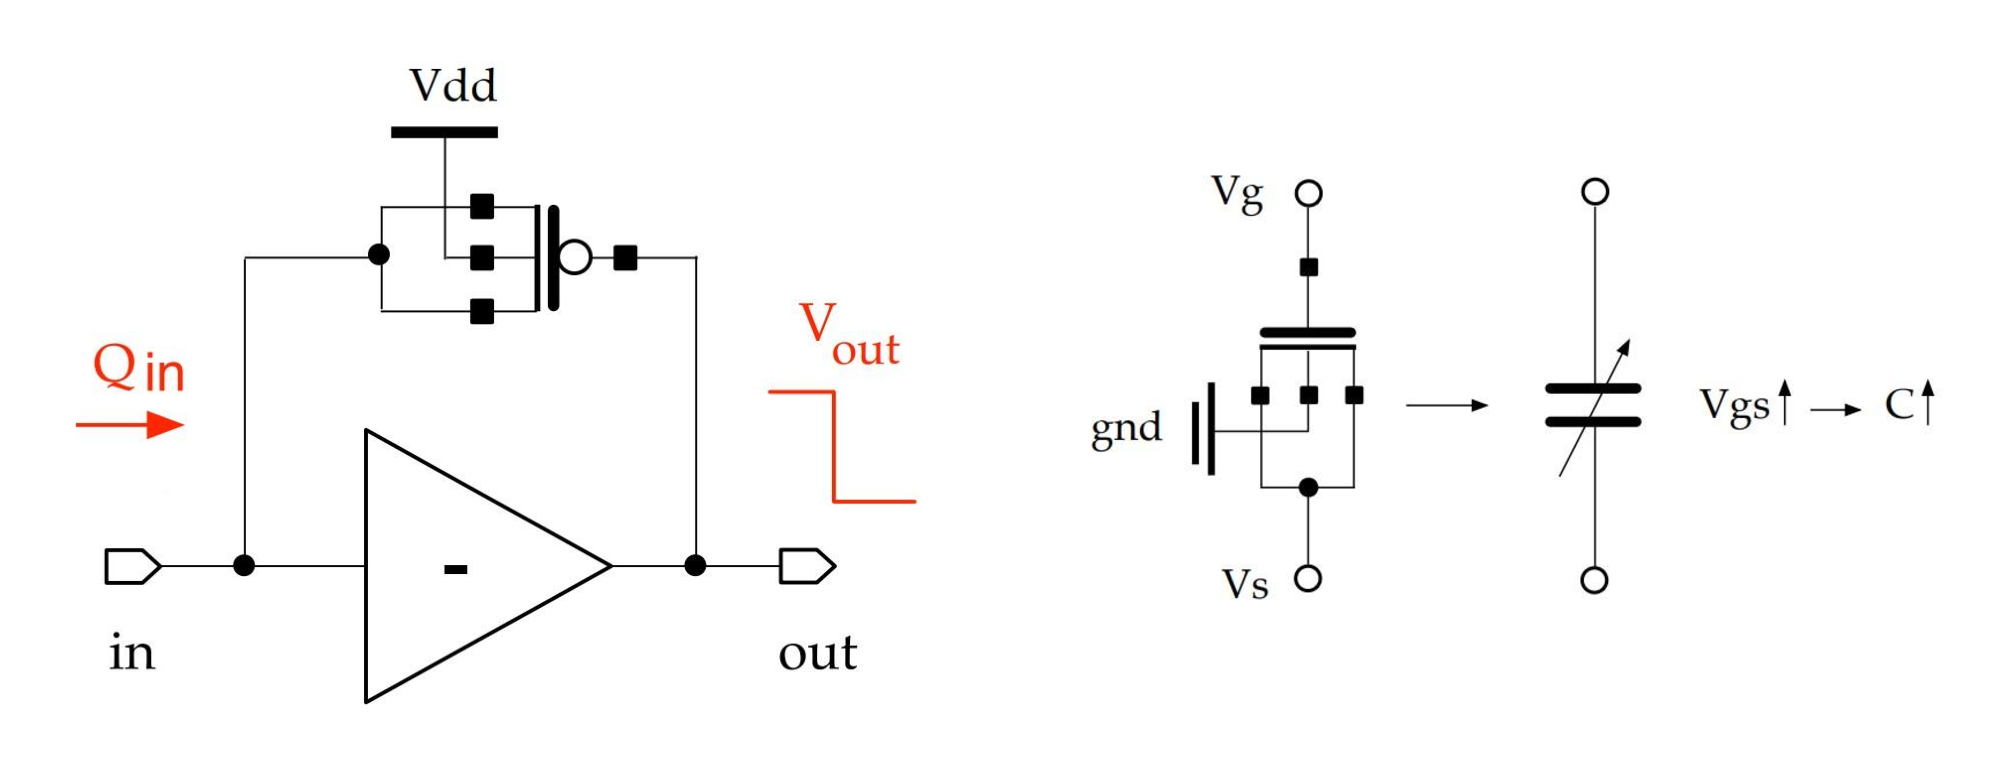
\includegraphics[width=0.9\textwidth]{images/backup_slides/dynamic_compression.pdf}
            \vspace{0.2cm}
            \begin{itemize}
                \item $0 < V_{GS} \ll V_{Th} \rightarrow C_{GS}$ is set at its minimum and it is mainly due to the overlap gate-to-source $C_{GS,ov}$ and gate-to-drain $C_{GD, ov}$ capacitances:
                \begin{equation*}
                    C_{min} \approx C_{GS,ov} + C_{GD,ov} = 2W\Delta L C_{OX}
                \end{equation*}
                \item $V_{GS} \gg V_{Th} \rightarrow C_{GS}$ shows a maximum value which is mainly given by the gate-to-channel $C_{GC}$ capacitance:
                \begin{equation*}
                    C_{max} \approx C_{GC} = WLC_{OX}
                \end{equation*}
            \end{itemize}
            \vspace{-0.25cm}
            \begin{equation*}
                Gain \propto \frac{1}{C_{f}}
            \end{equation*}
    \end{columns}  
\end{frame}


%---------------------------------------------------------------------------------------
%	Front-end and Flex-rigid boards
%---------------------------------------------------------------------------------------

\begin{frame}{Front-end and Flex-rigid boards}
    \fontsize{8.5pt}{1}\selectfont
    \settowidth{\leftmargini}{\usebeamertemplate{itemize item}}
    \addtolength{\leftmargini}{\labelsep}
    \begin{columns}
        \column{0.45\textwidth}
            \vskip0.1cm
            \fontsize{9.5pt}{1}\selectfont
            \textbf{\textcolor{Red}{Front-end board}}
            \fontsize{8.5pt}{1}\selectfont
            \begin{itemize}
                \setlength\itemsep{0.2em}
                \item One ASIC connected to 4 Si(Li) detectors
                \vspace{-0.15cm}
                \item Voltage regulators and filtering for
                    \begin{itemize}
                        \fontsize{8.5pt}{1}\selectfont
                        \item Si(Li) detector High Voltage Power Supply
                        \item ASIC Low Voltage Power Supply (AVDD, DVDD)
                    \end{itemize}
                \item ASIC SPI control signals
                \item ADC clock
                \item Temperature sensor
                \item ASIC calibration system (16 bit DAC)
            \end{itemize}
            \vspace{0.1cm}
            \fontsize{9.5pt}{1}\selectfont
            \textbf{\textcolor{Red}{Flex-rigid board}}
            \fontsize{8.5pt}{1}\selectfont
            \begin{itemize}
                \setlength\itemsep{0.2em}
                \item Connects Front-end boards in series
                \vspace{-0.15cm}
                \item Propagates
                    \begin{itemize}
                        \fontsize{8.5pt}{1}\selectfont
                        \item ASIC Low Voltage Power Supply
                        \item SPI control signals and ADC clock
                    \end{itemize}
            \end{itemize}
            \centering
            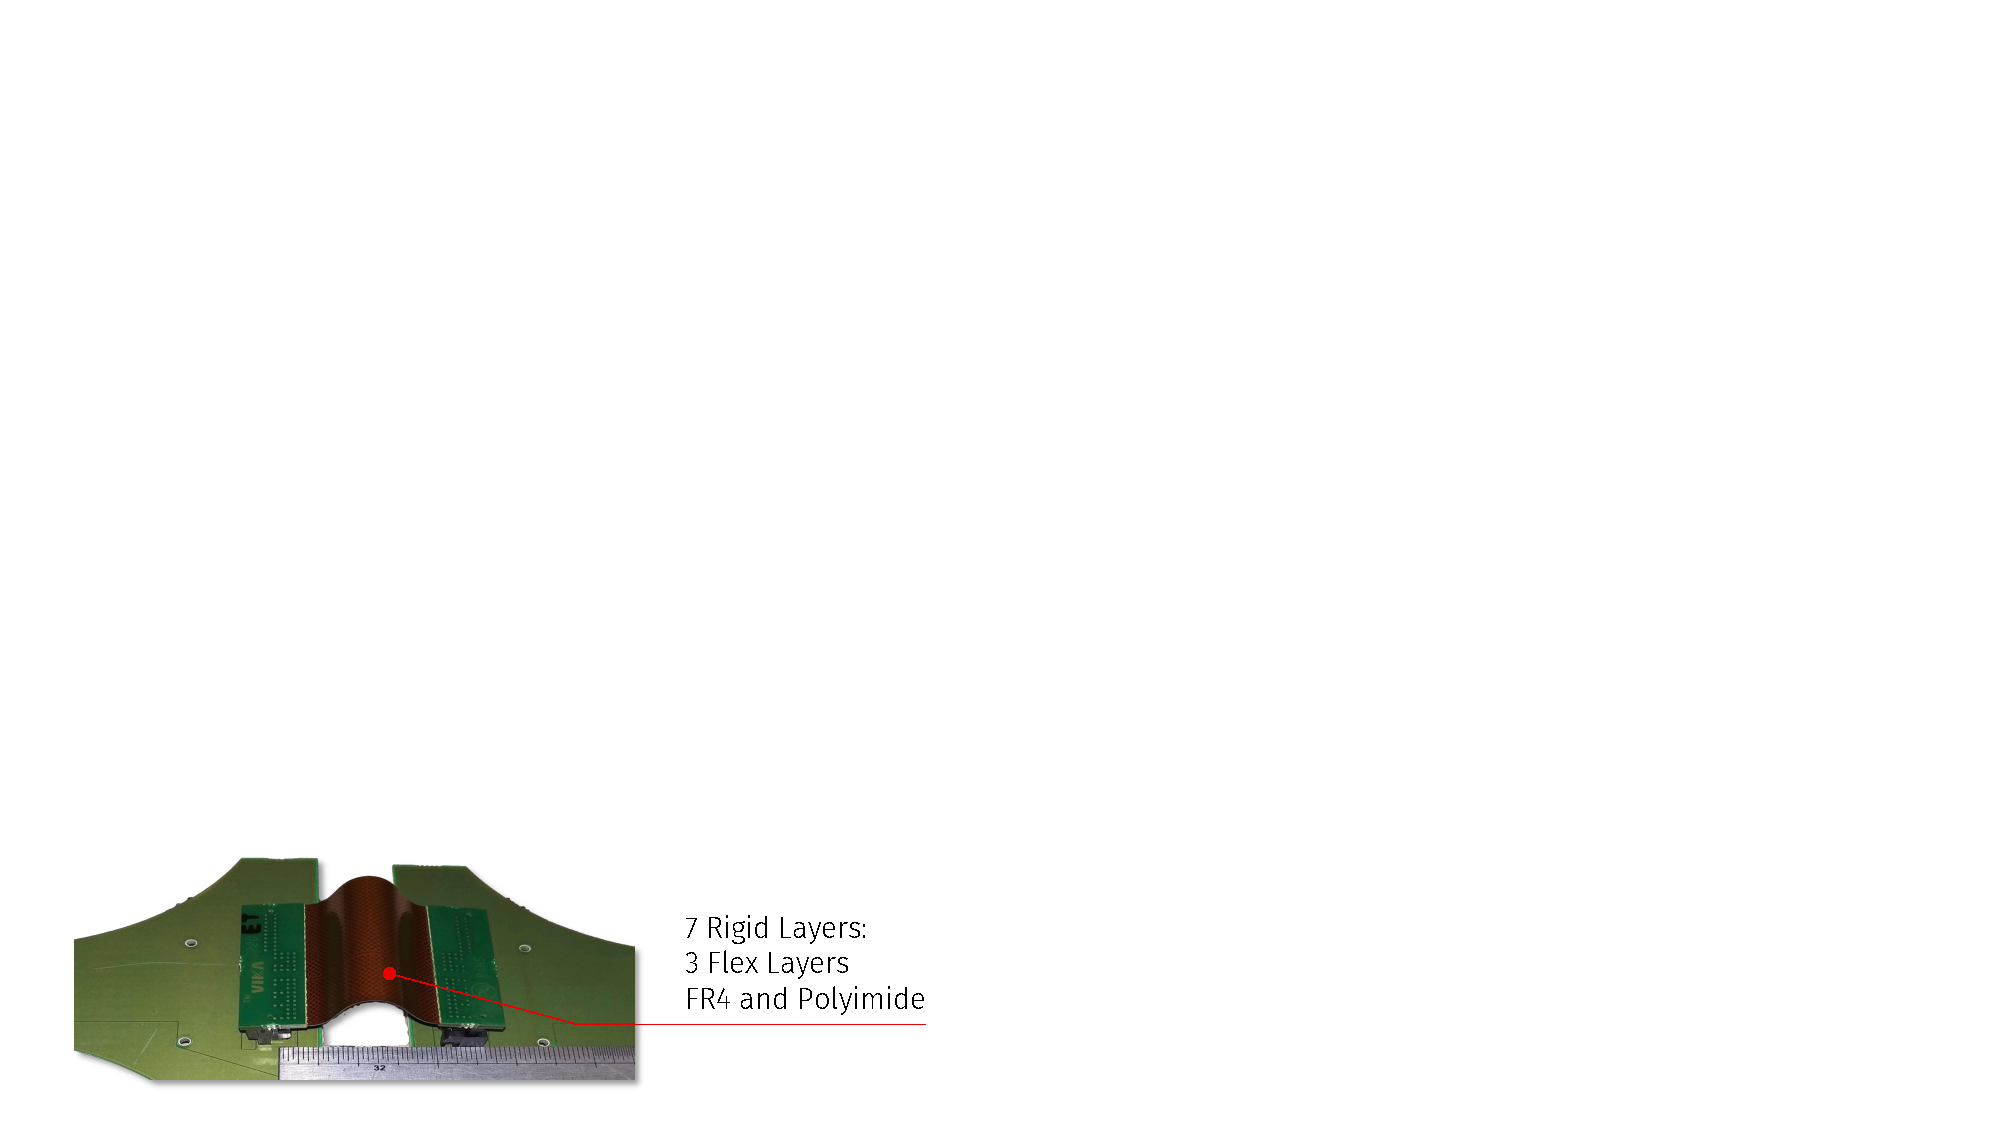
\includegraphics[width=0.97\textwidth]{images/backup_slides/flex_rigid_description.pdf}  
        \column{0.5\textwidth}
            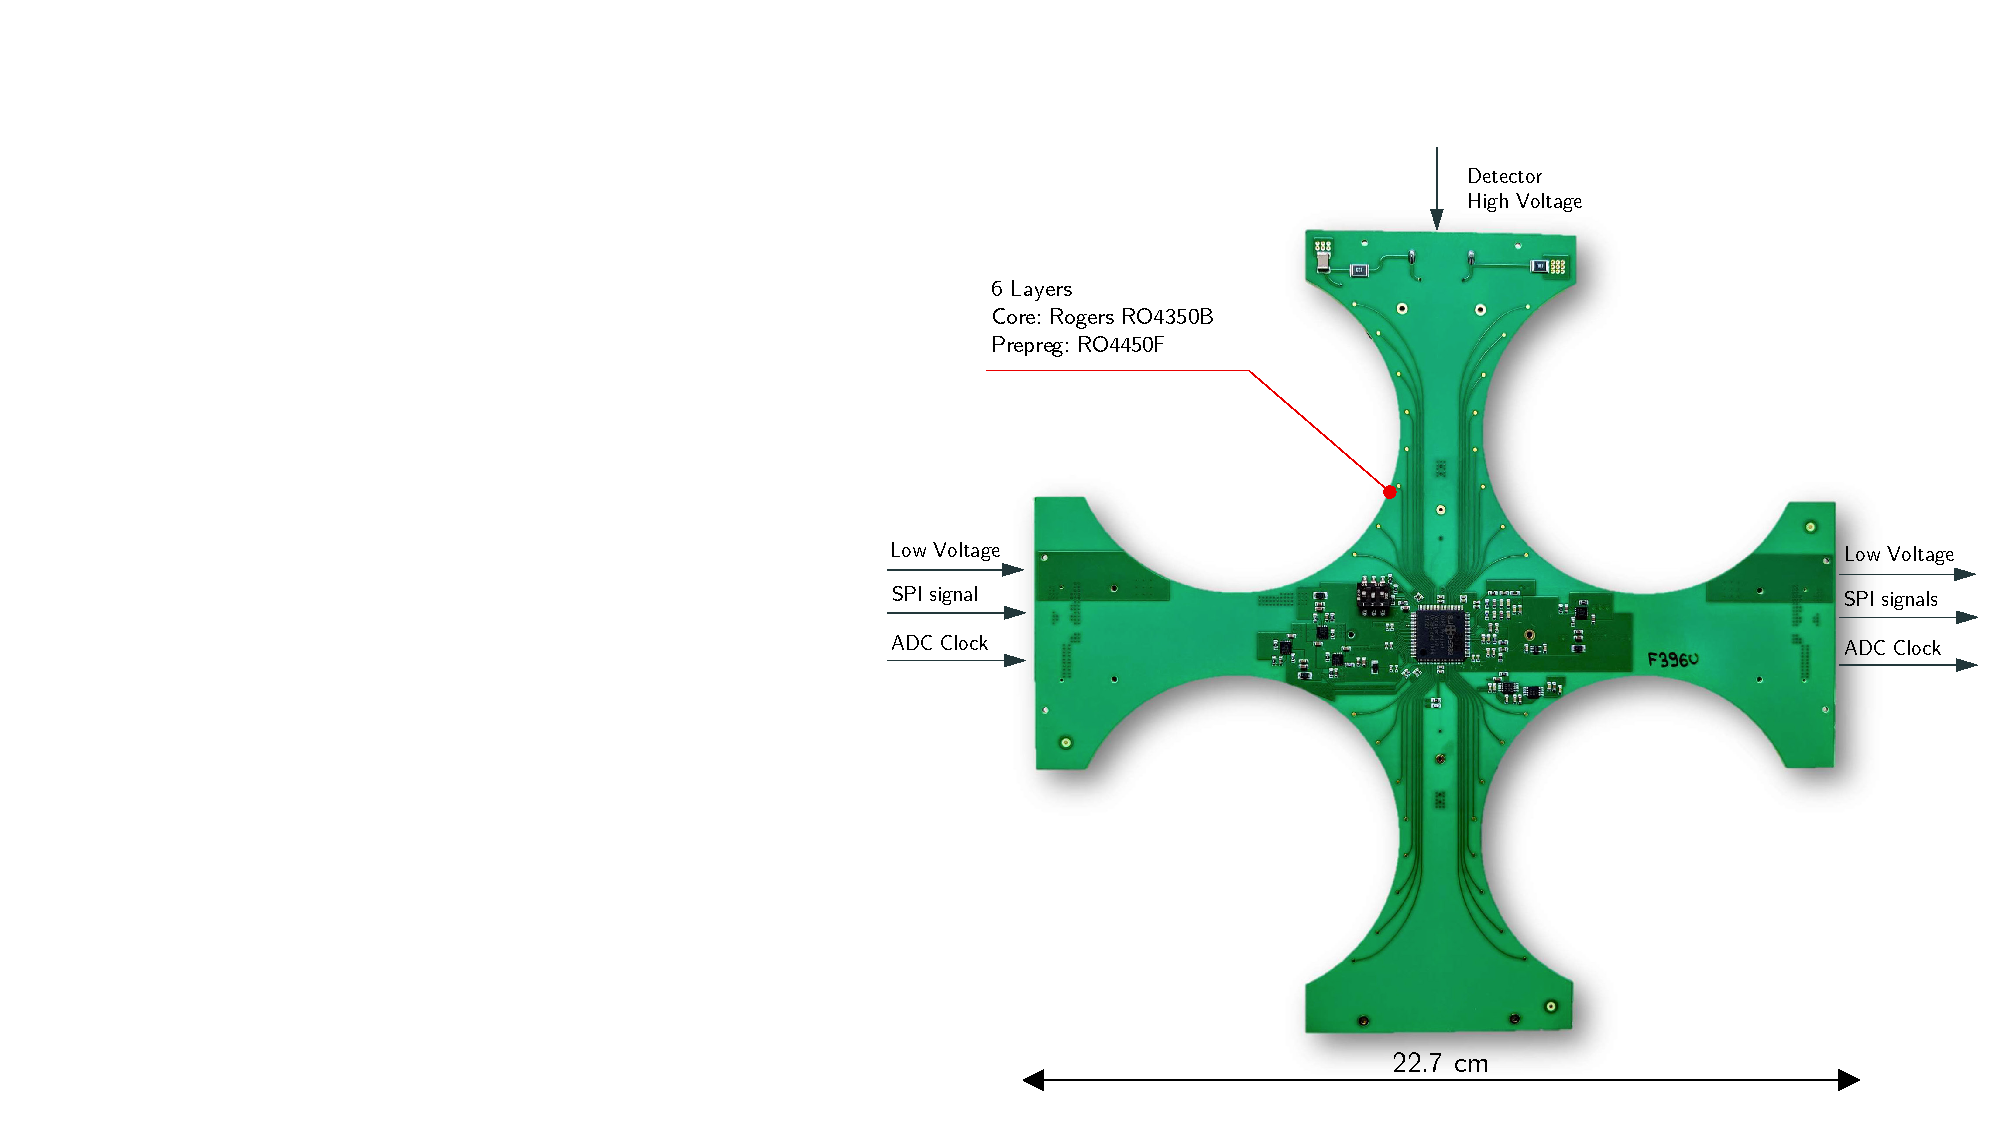
\includegraphics[width=1.05\textwidth]{images/backup_slides/feb_signals.pdf}
            \vspace{0.4cm}  
    \end{columns}
\end{frame}

\begin{frame}{A row of 6 modules}
    \begin{columns}
        \column{0.4\textwidth}
            \centering
            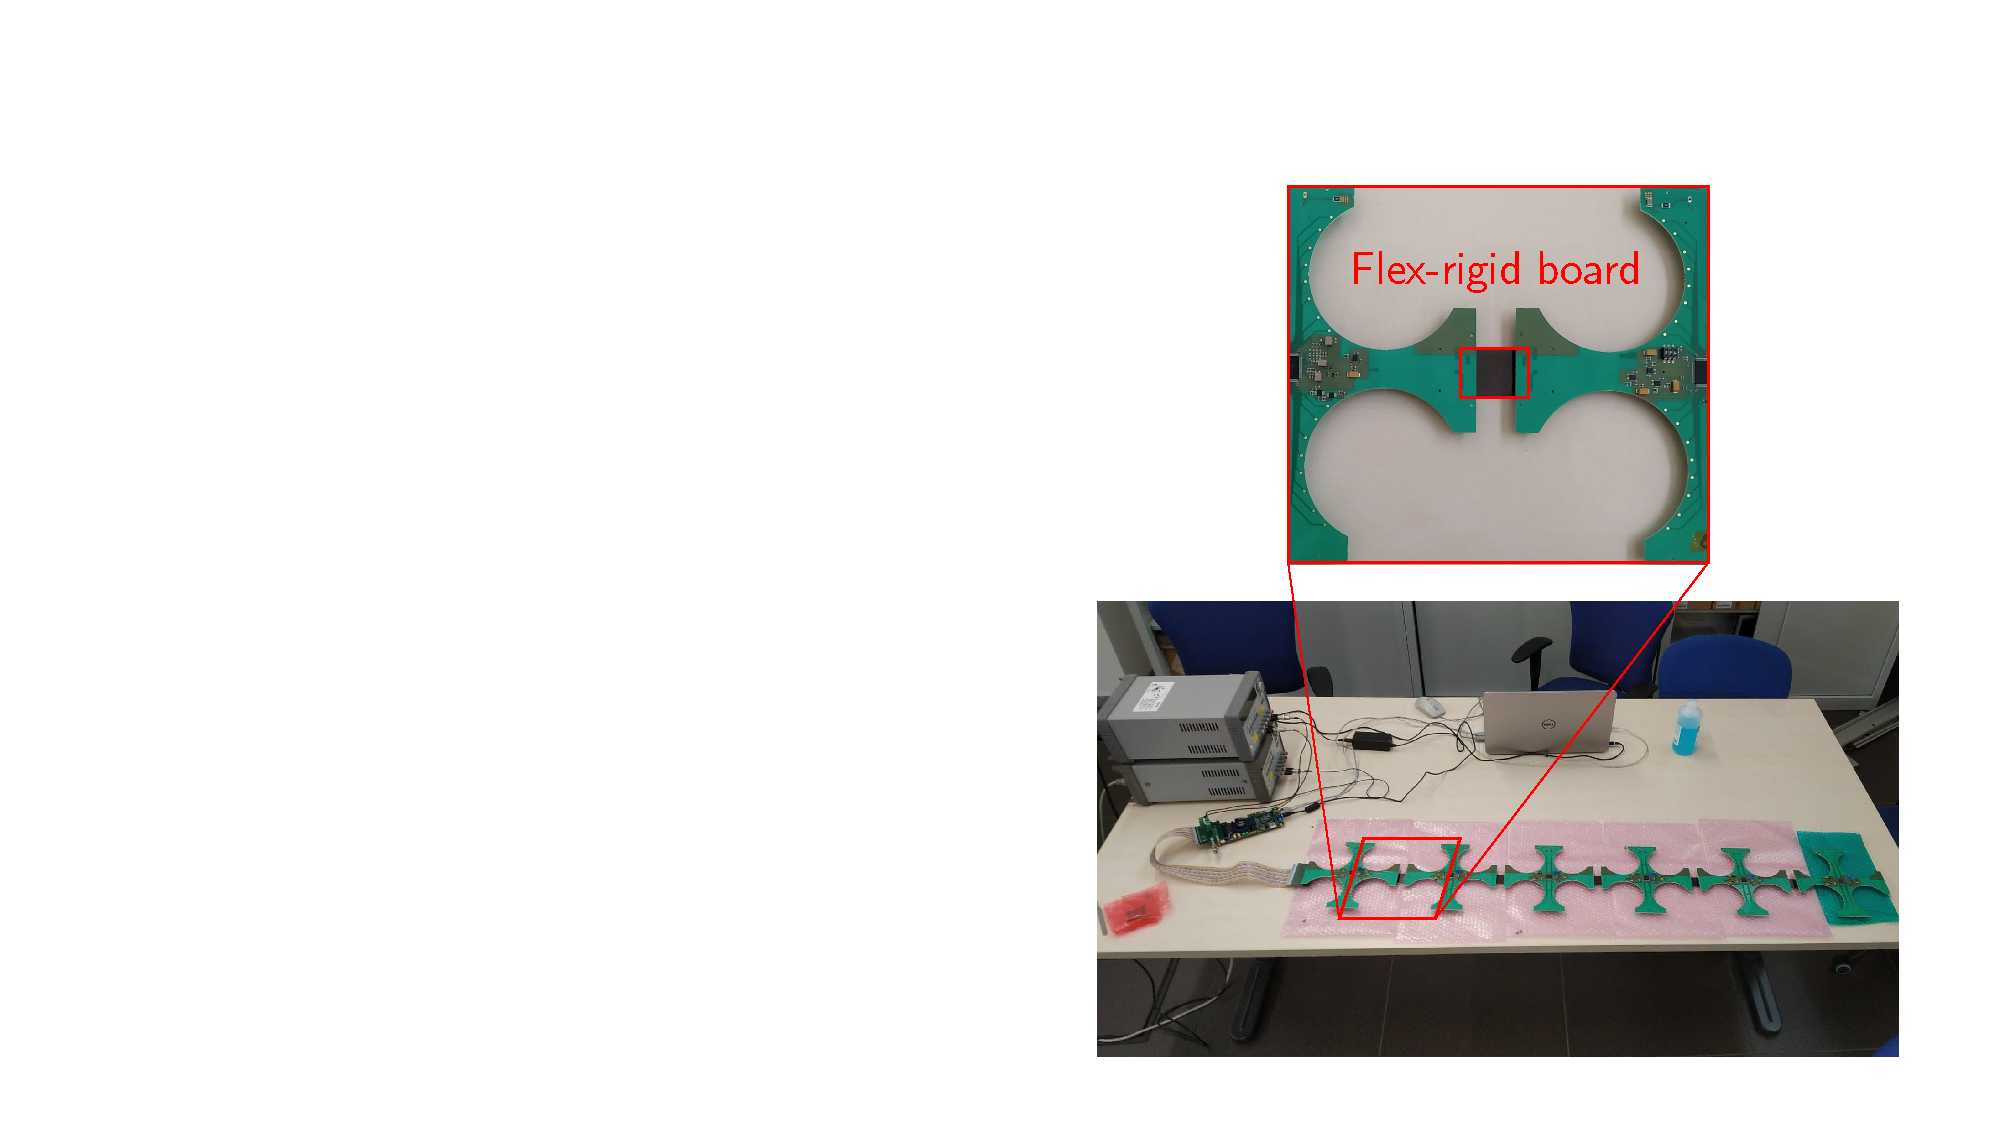
\includegraphics[width=1\textwidth]{images/backup_slides/flex_paolo.pdf}

        \column{0.55\textwidth}
            \centering
            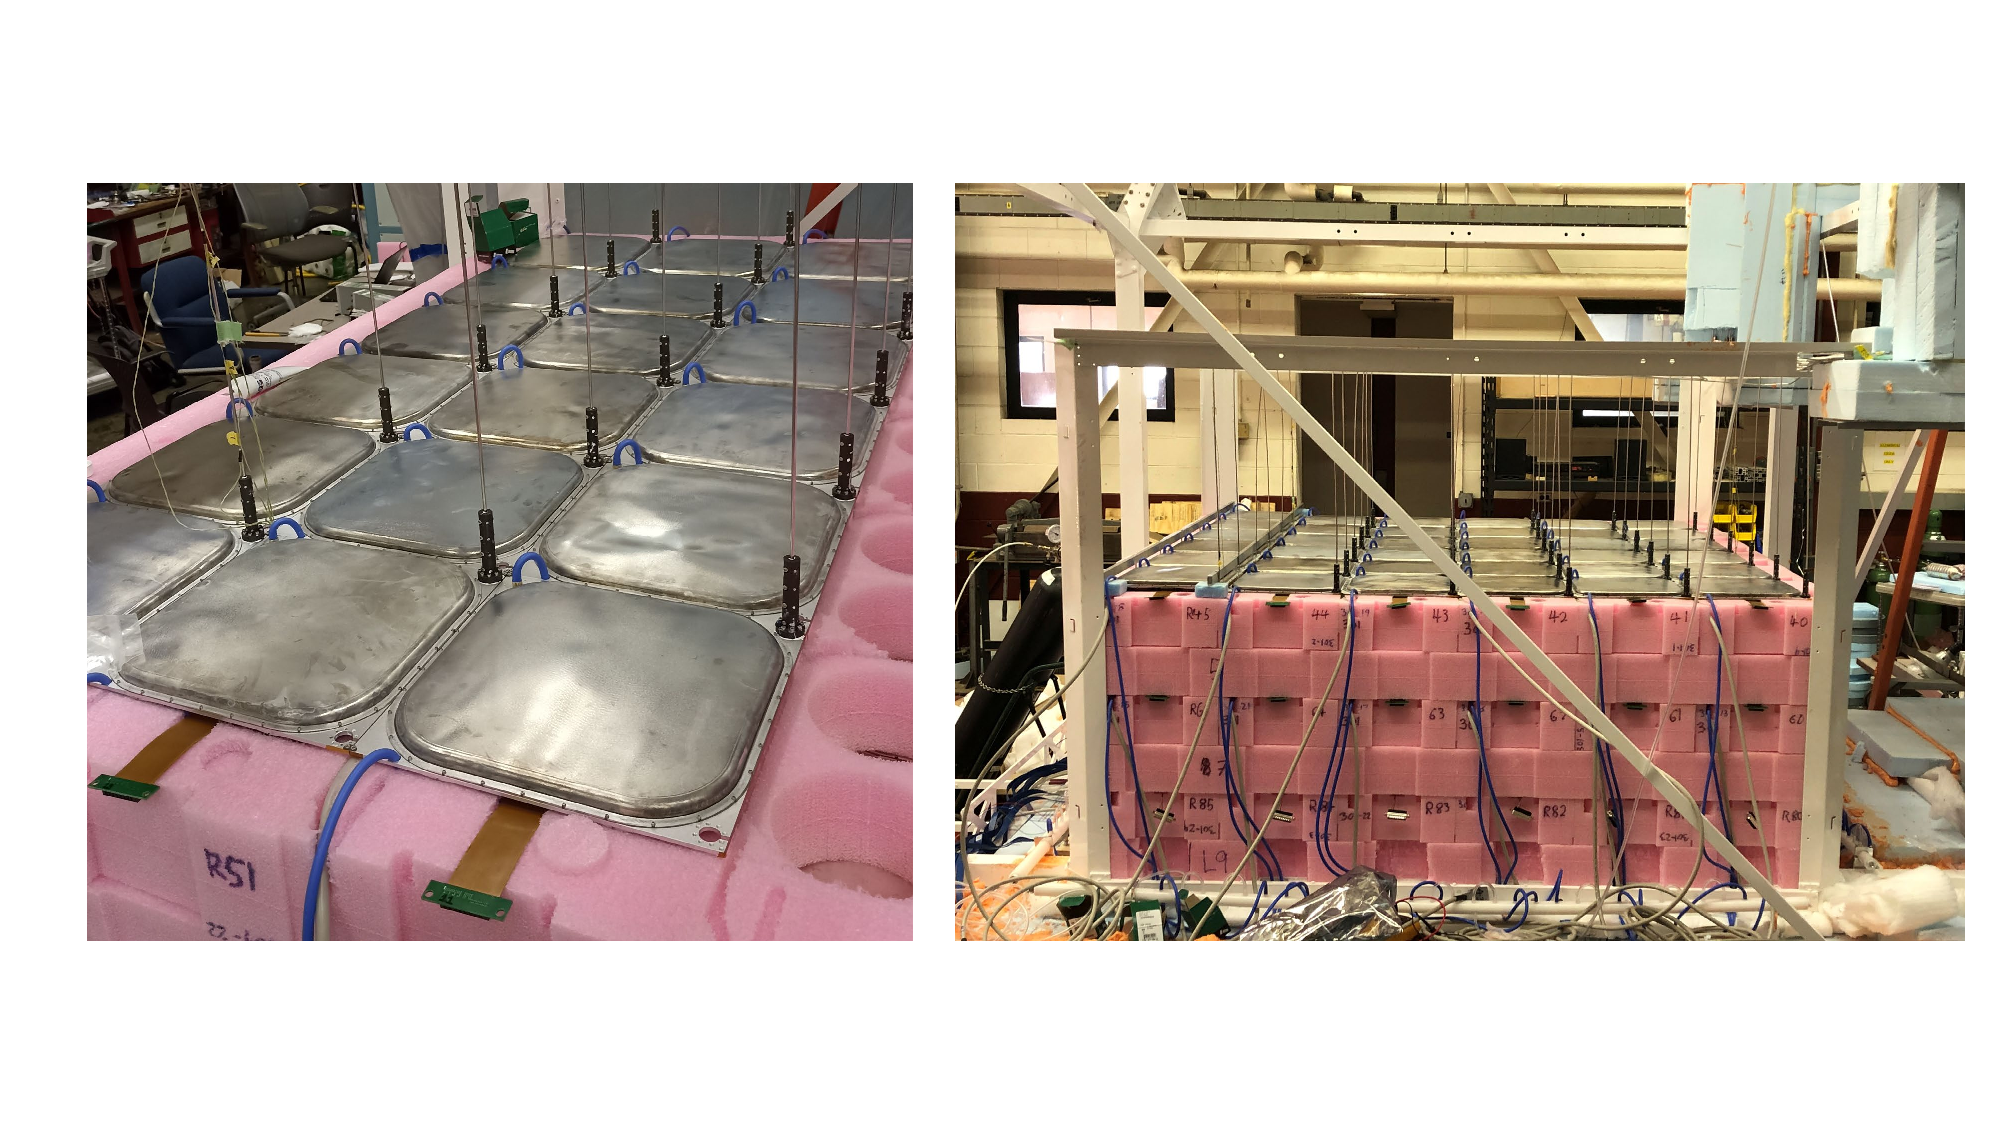
\includegraphics[width=1\textwidth]{images/backup_slides/row_feb_coppia.pdf}
            \vskip0.2cm
            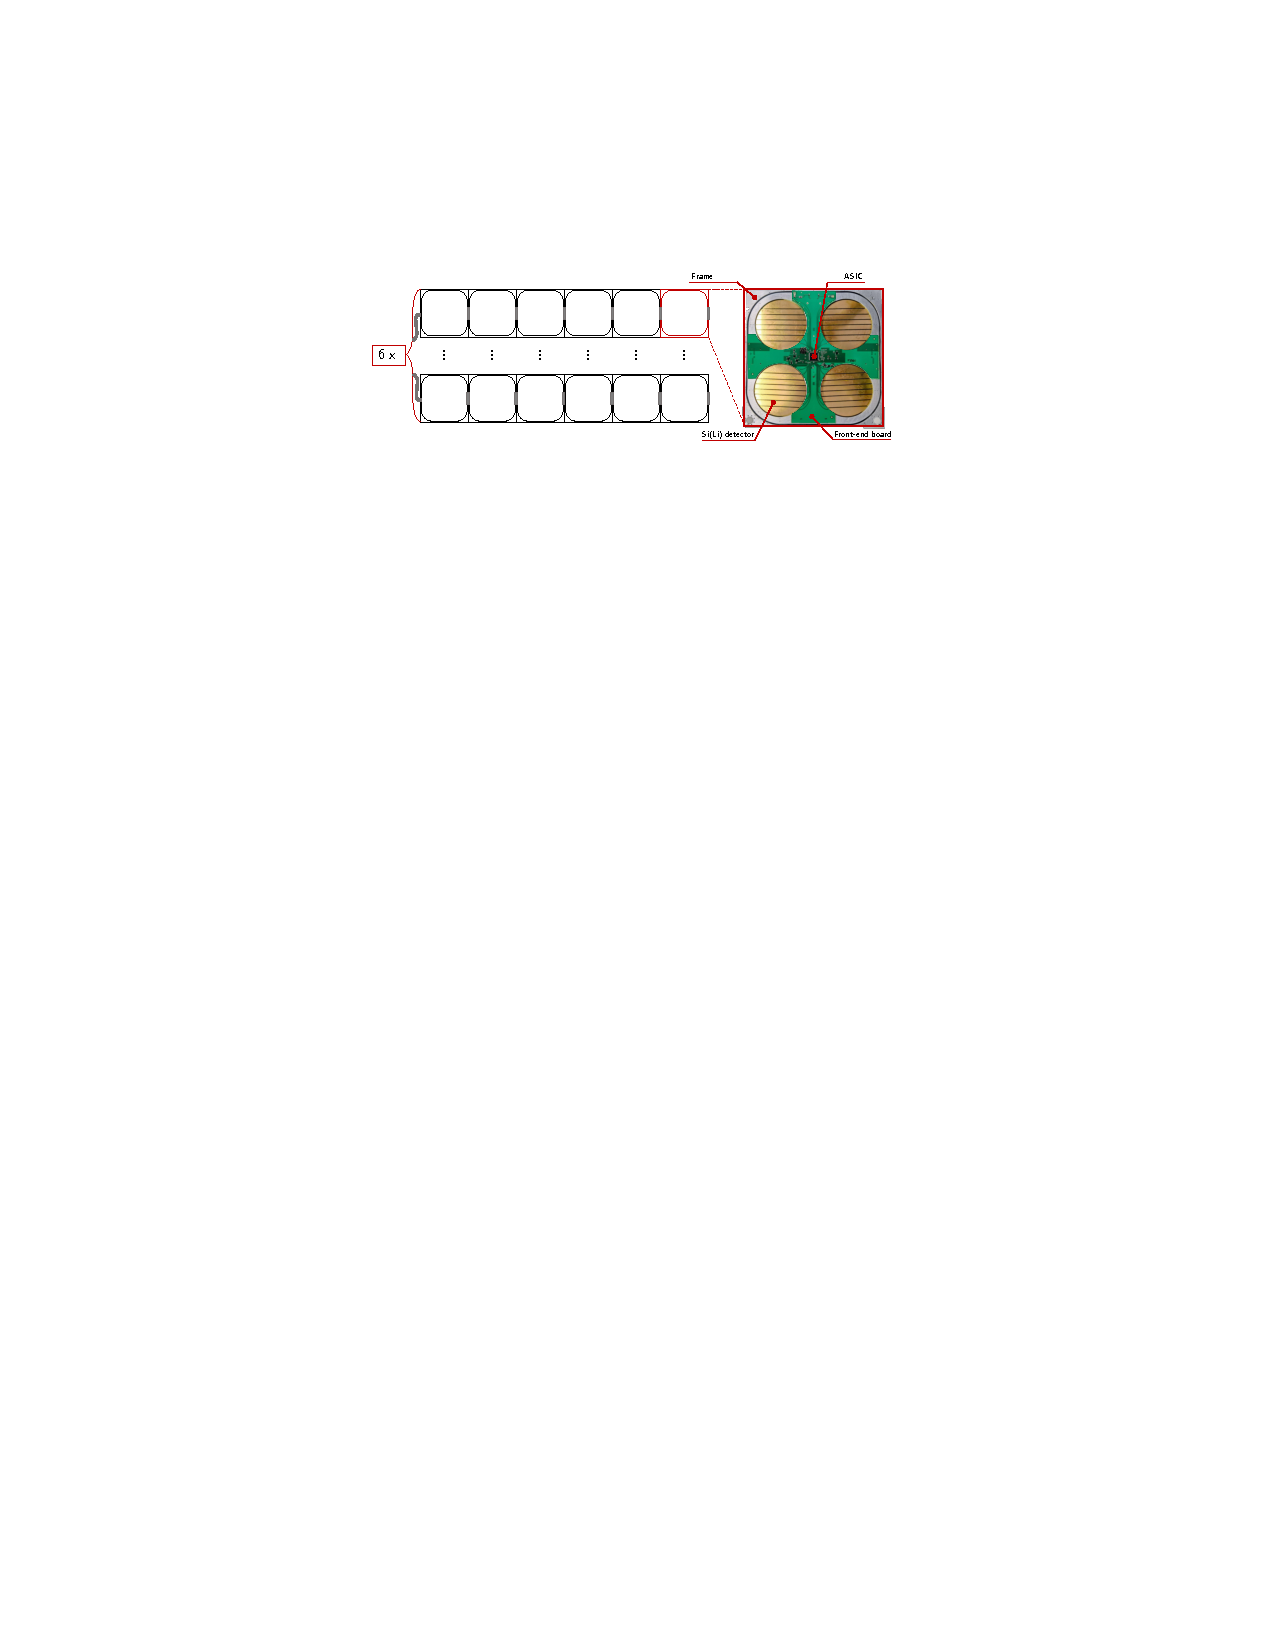
\includegraphics[width=1\textwidth]{images/backup_slides/row_scheme_elisa.pdf}   
    \end{columns}
\end{frame}

\begin{frame}{Front-end board shields}
    \settowidth{\leftmargini}{\usebeamertemplate{itemize item}}
    \addtolength{\leftmargini}{\labelsep}
    \fontsize{9pt}{1}\selectfont
    \begin{columns}
        \column{0.45\textwidth}
            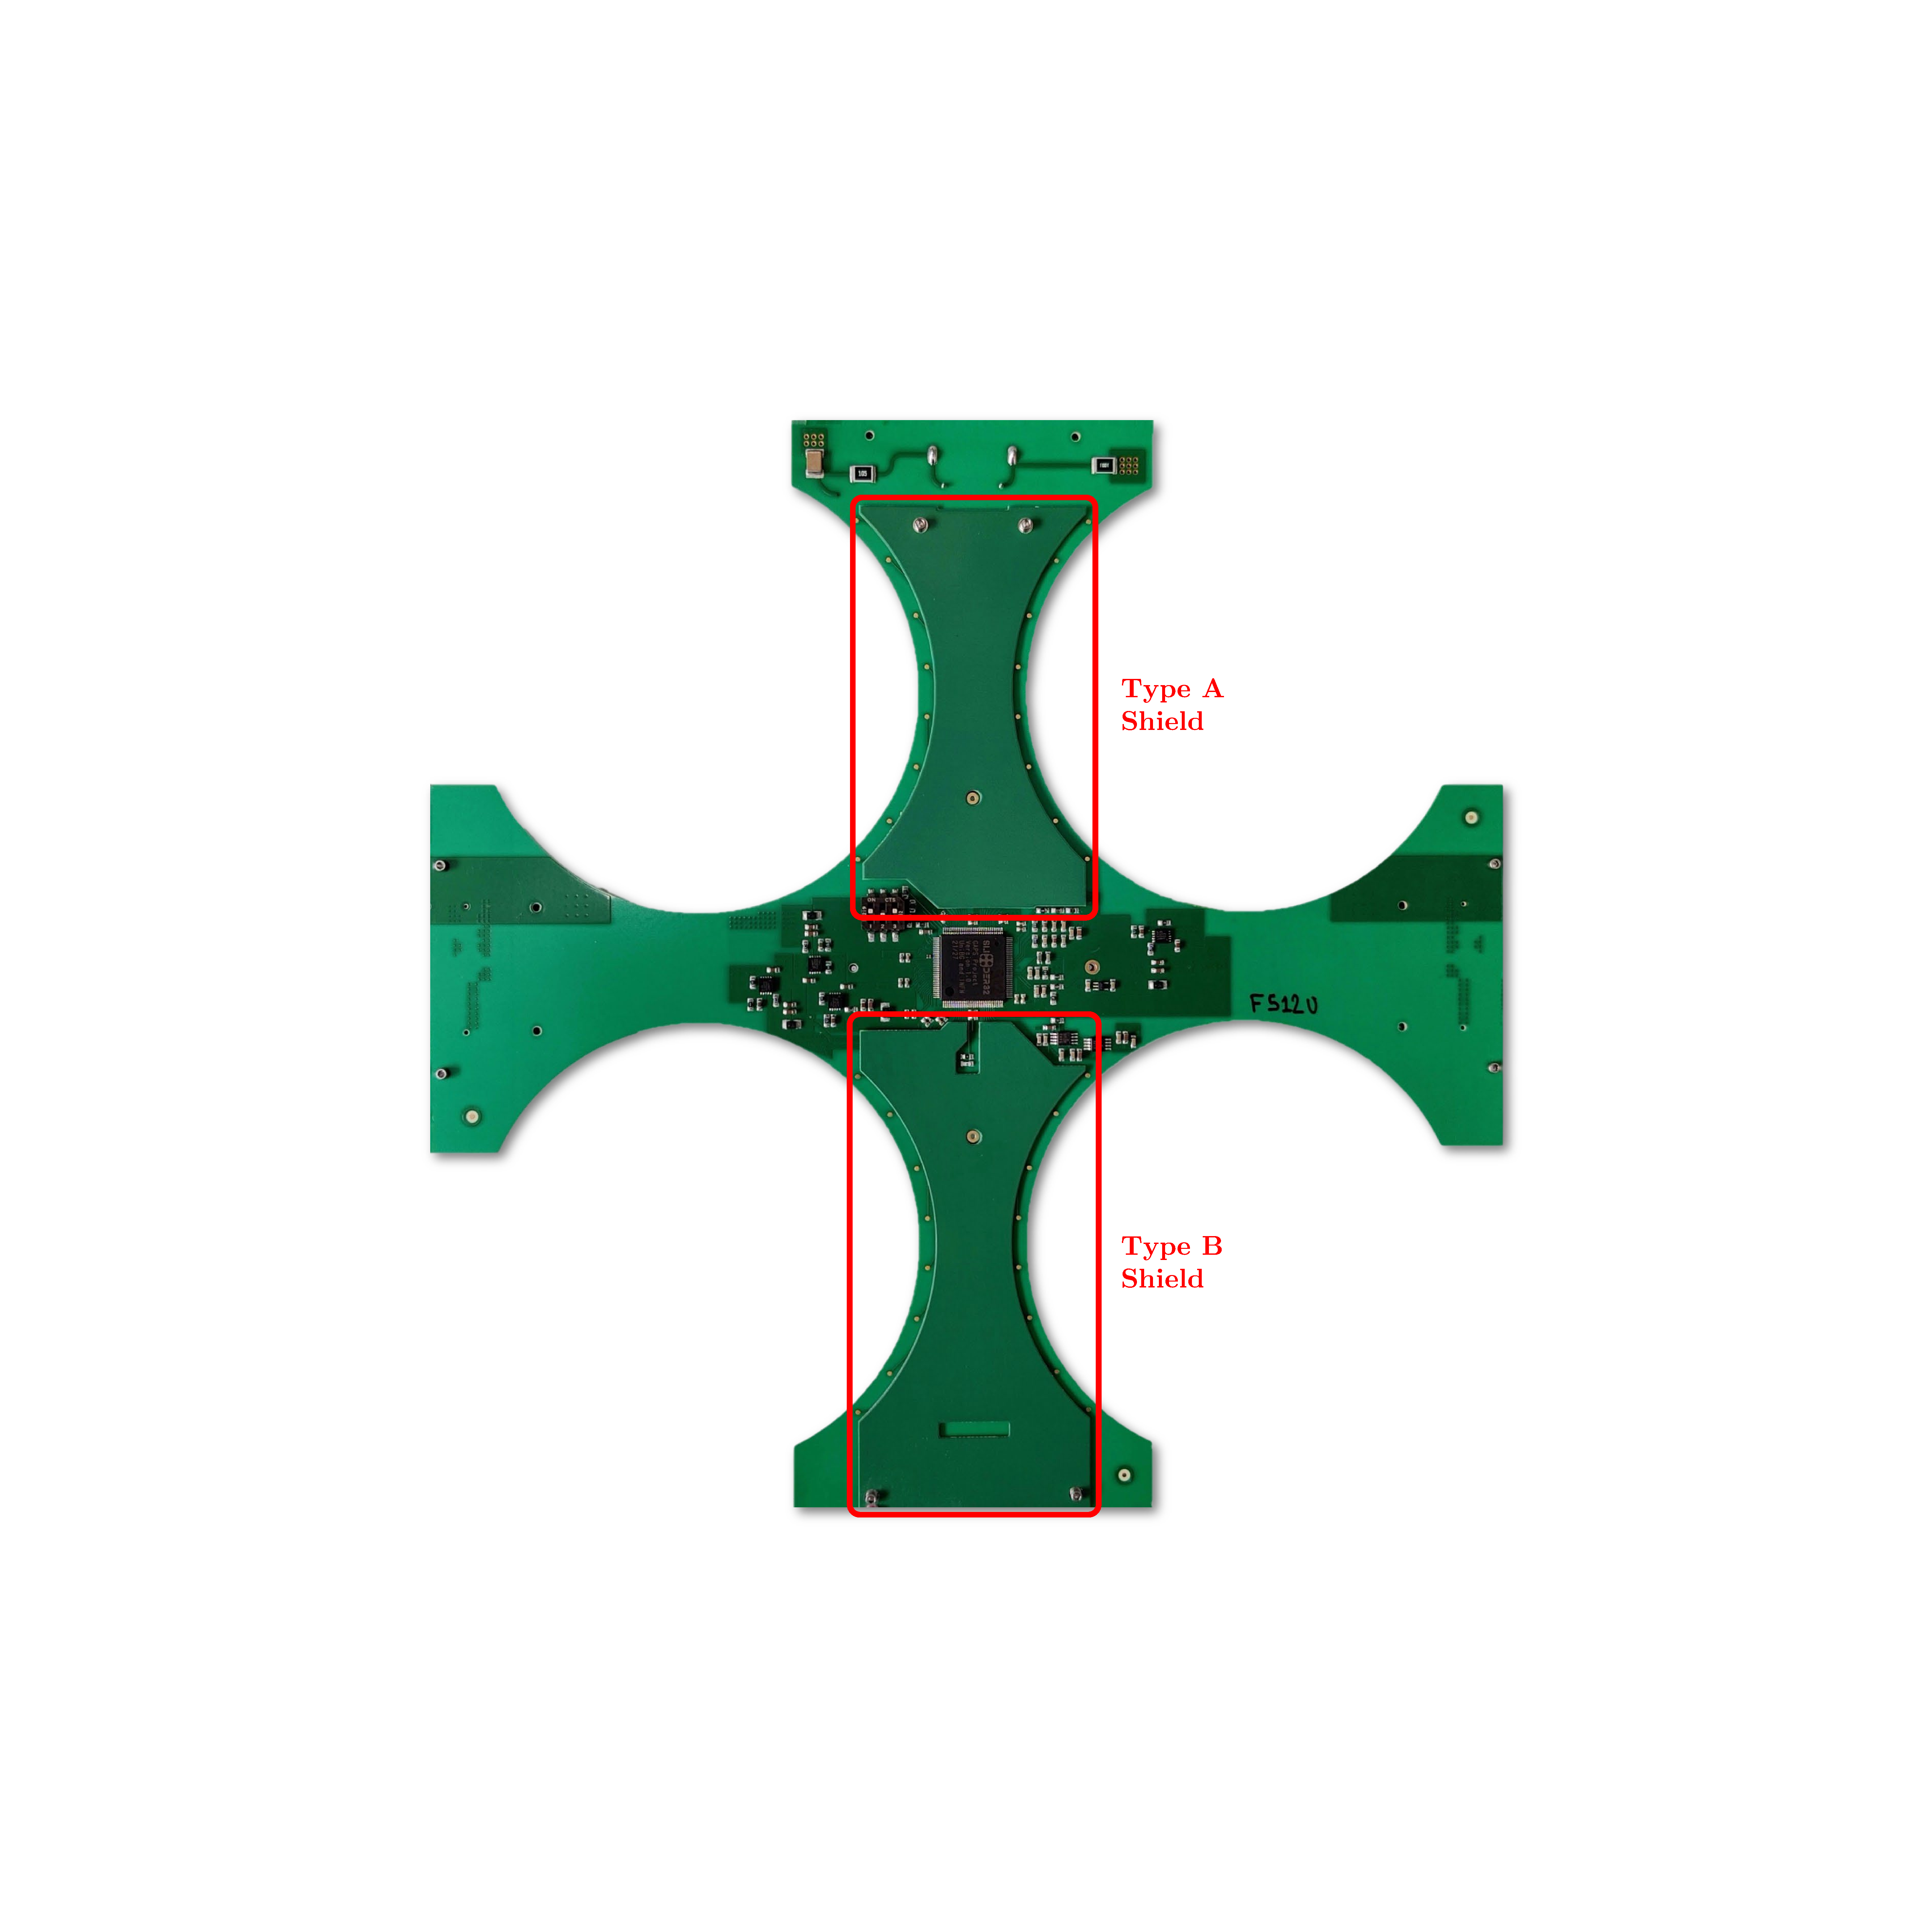
\includegraphics[width=1\textwidth]{images/backup_slides/FEB_with_shields.pdf}
            
        \column{0.49\textwidth}
            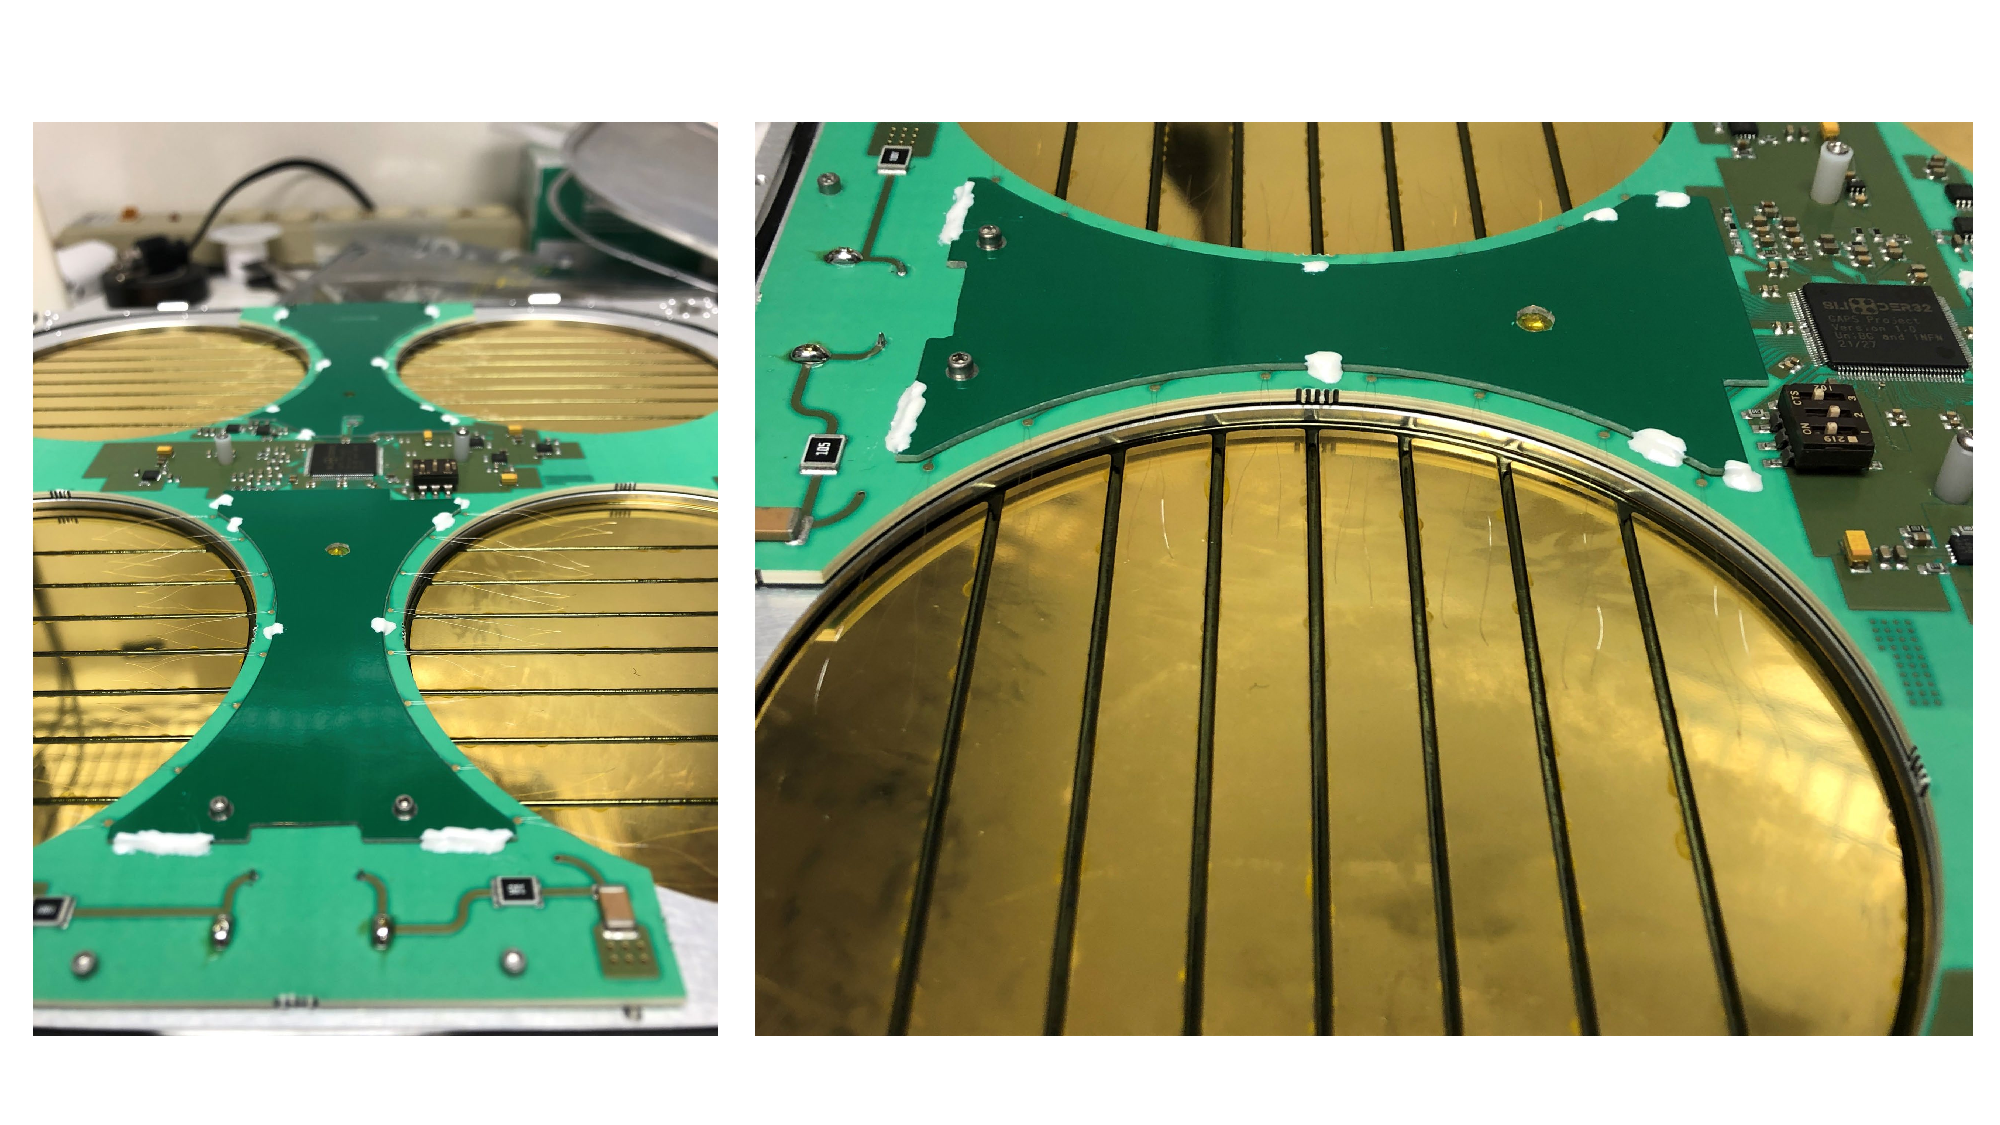
\includegraphics[width=0.99\textwidth]{images/backup_slides/shields_menjiao_coppia.pdf}

            \vskip0.3cm
            \begin{itemize}
                \item \textbf{Type A} and \textbf{Type B} front-end board shields
                \item Designed with metal plane connected to ground
                \item Installed on front-end board over tracks connecting Si(Li) detector strips to ASIC
                \item \textcolor{Red}{\textbf{Problem:}} long tracks acting as antennas for disturbances of electromagnetic nature
                \item \textcolor{ForestGreen}{\textbf{Solution:}} cover tracks with shields to lower the noise
            \end{itemize}
    \end{columns}
    
\end{frame}

\begin{frame}{Front-end board test setup}
    \begin{columns}
        \column{0.48\textwidth}
            \fontsize{9pt}{1}\selectfont
            \textcolor{Red}{\textbf{Test setup}}
            \begin{itemize}
                \fontsize{8.5pt}{1}\selectfont
                \item FEB or 6 FEBs connected by 5 flex-rigid boards
                \item Termination connector to close the row
                \item FPGA Intel Cyclone V (\SI{48}{\mega\hertz} clock frequency)
                \item Interface board, flex-ribbon cable and adapter board for connecting FPGA to FEB
                \item Keysight N6705C DC power supply, providing analog, digital and calibration 
                \item PC connected via USB to FPGA
                \item Purposely developed Python software to perform test on FEB and acquire data
                \item MATLAB script to elaborate data and plot results
            \end{itemize}

            \vspace{0.15cm}
            \fontsize{9pt}{1}\selectfont
            \textcolor{Red}{\textbf{Tests performed}}
            \begin{itemize}
                \item Automated test performed via dedicated Python script
                \item Voltage measurements on FEB taken with multimeter
            \end{itemize}

        \column{0.48\textwidth}
            \centering
            \vskip0.1cm
            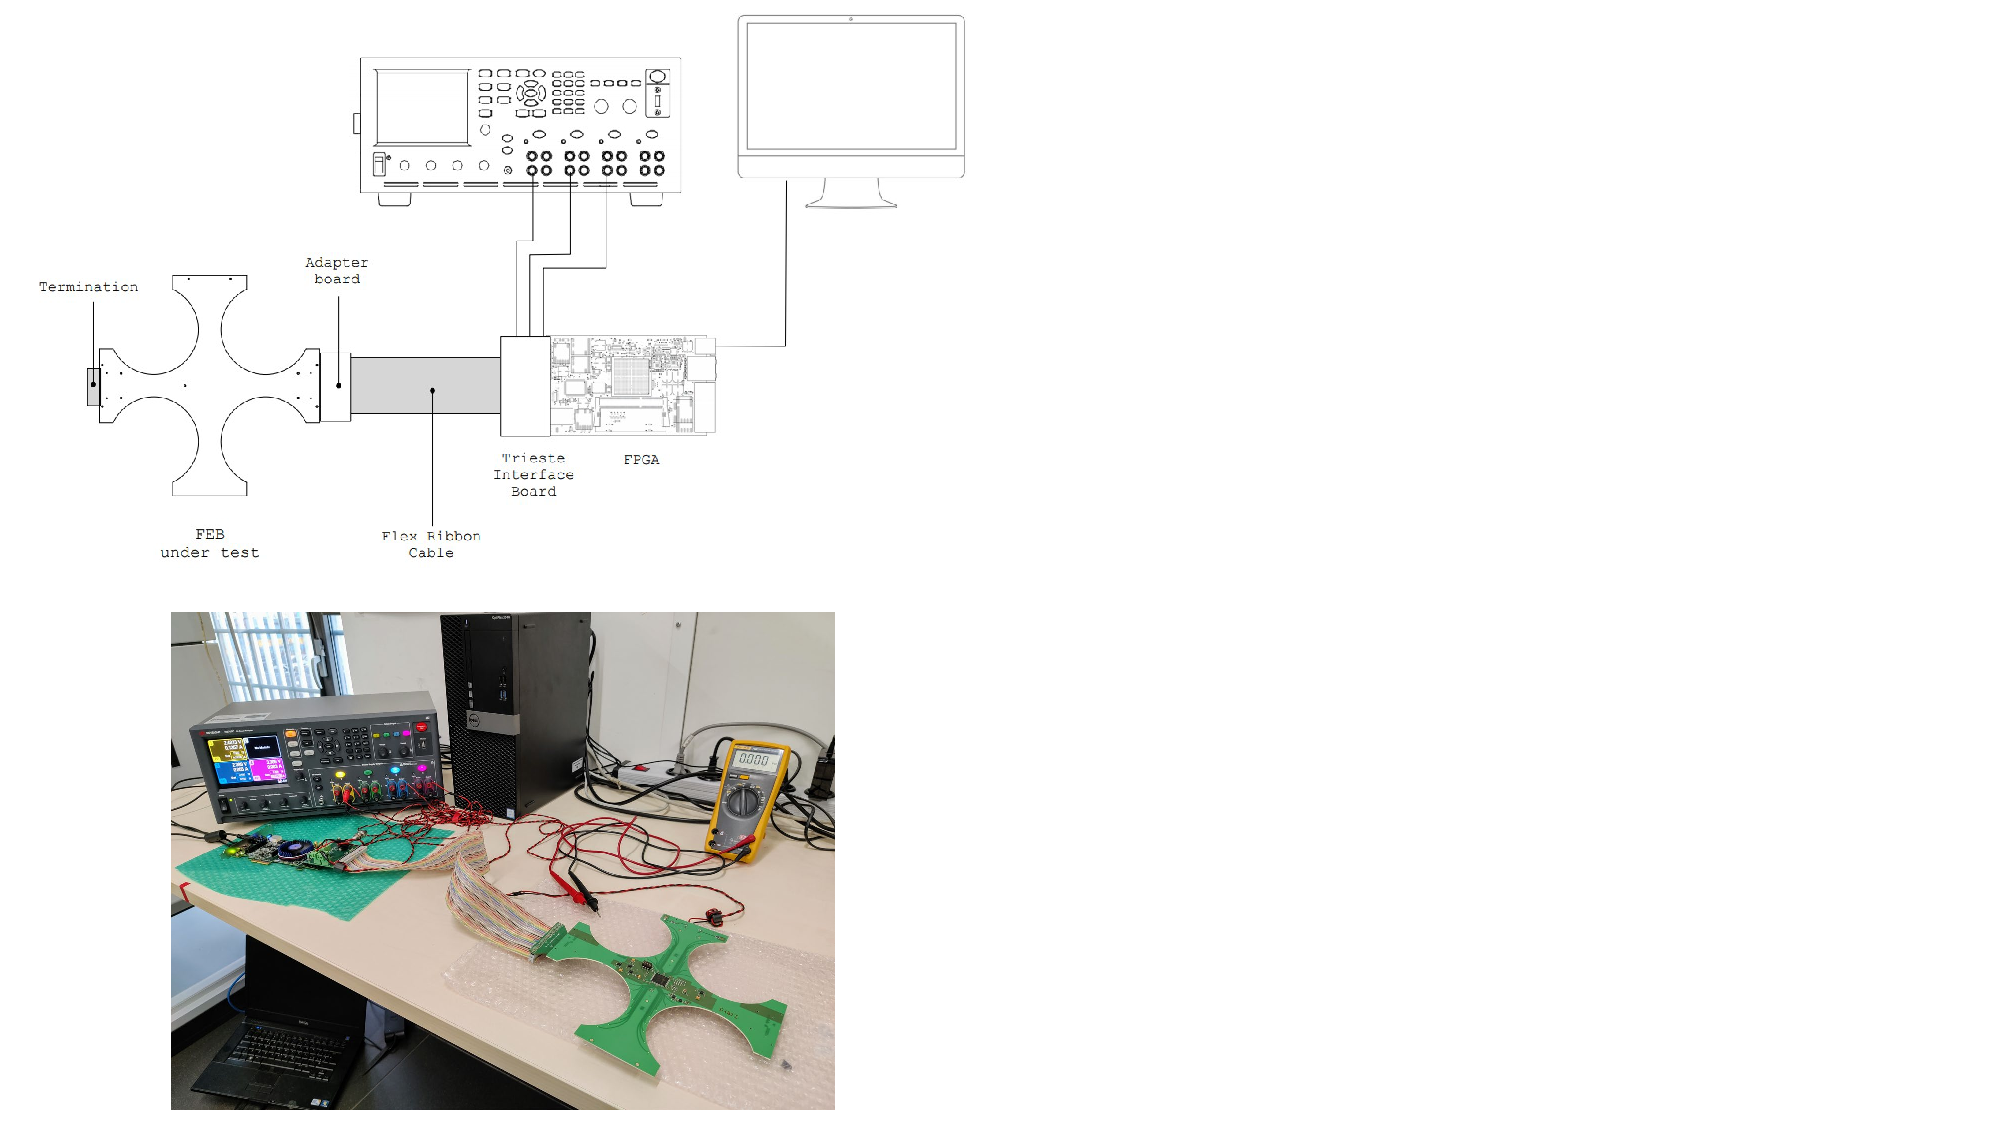
\includegraphics[height=0.85\textheight]{images/backup_slides/FEB_setup_combo.pdf}
            
    \end{columns}
    
\end{frame}

\begin{frame}{Threshold setting for X-ray detection}
    \begin{columns}[T]
        \column{0.475\textwidth}
            \centering
             \fontsize{9pt}{1}\selectfont
            \textbf{\textcolor{ForestGreen}{Charge scan performed on Si(Li) detector \#0}}\\
             \fontsize{8.5pt}{1}\selectfont
             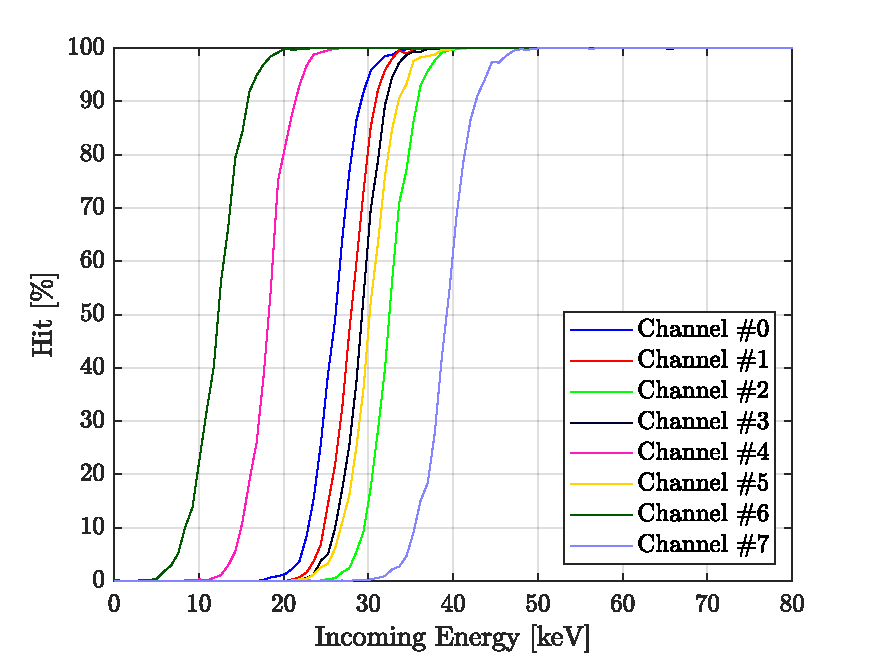
\includegraphics[height=0.55\textheight]{images/backup_slides/Threshold Scan - Detector 0 - TH214.pdf}
             \vspace{0.1cm}
            \begin{itemize}
                \item Detector \#0: channels 0 to 7
                \item \textbf{Goal:} determine THR value to detect \ce{^{241}Am} X-ray peaks at \SI{26.34}{\kilo\electronvolt} and \SI{59.54}{\kilo\electronvolt}
                \item Channel's trigger profile obtained keeping THR constant and varying injected charge
            \end{itemize}

        \column{0.475\textwidth}
            \centering
            \fontsize{9pt}{1}\selectfont
            \textbf{\textcolor{ForestGreen}{Threshold \& ENC obtained from charge scan}}\\
            \fontsize{8.5pt}{1}\selectfont
            \vskip0.26cm
            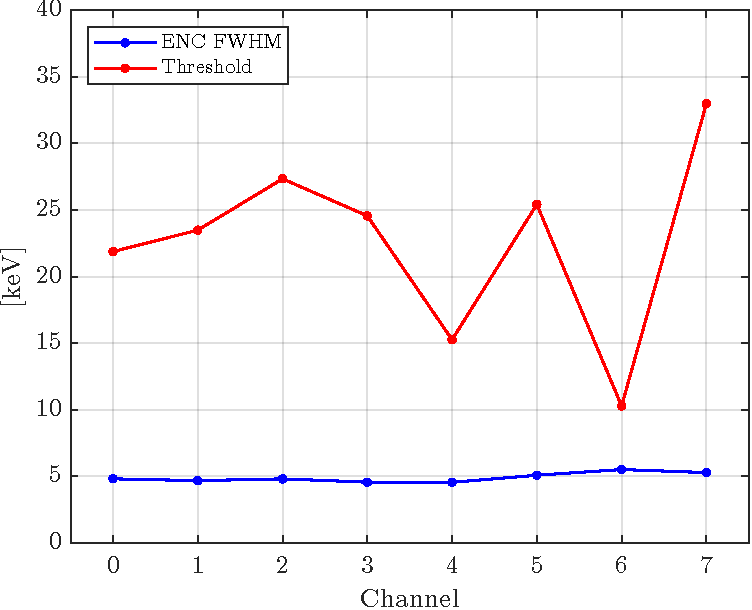
\includegraphics[height=0.515\textheight]{images/backup_slides/ENC_channels.pdf}
            \vspace{0.15cm}
            \begin{itemize}
                \item Threshold and ENC values for each channel extracted by interpolating Gaussian CDF
                \item Mean threshold equivalent to \textbf{\SI{22.65}{\kilo\electronvolt}}
                \item \textcolor{Red}{\textbf{Channel 6:}} \textbf{\SI{10.29}{\kilo\electronvolt}} threshold
                \item \textcolor{Red}{\textbf{Channel 7:}} \textbf{\SI{32.98}{\kilo\electronvolt}} threshold
            \end{itemize}
    \end{columns}
    
\end{frame}

\begin{frame}{Si(Li) detectors leakage current measurement}
    \begin{columns}[T]
        \column{0.6\textwidth}
            \centering
            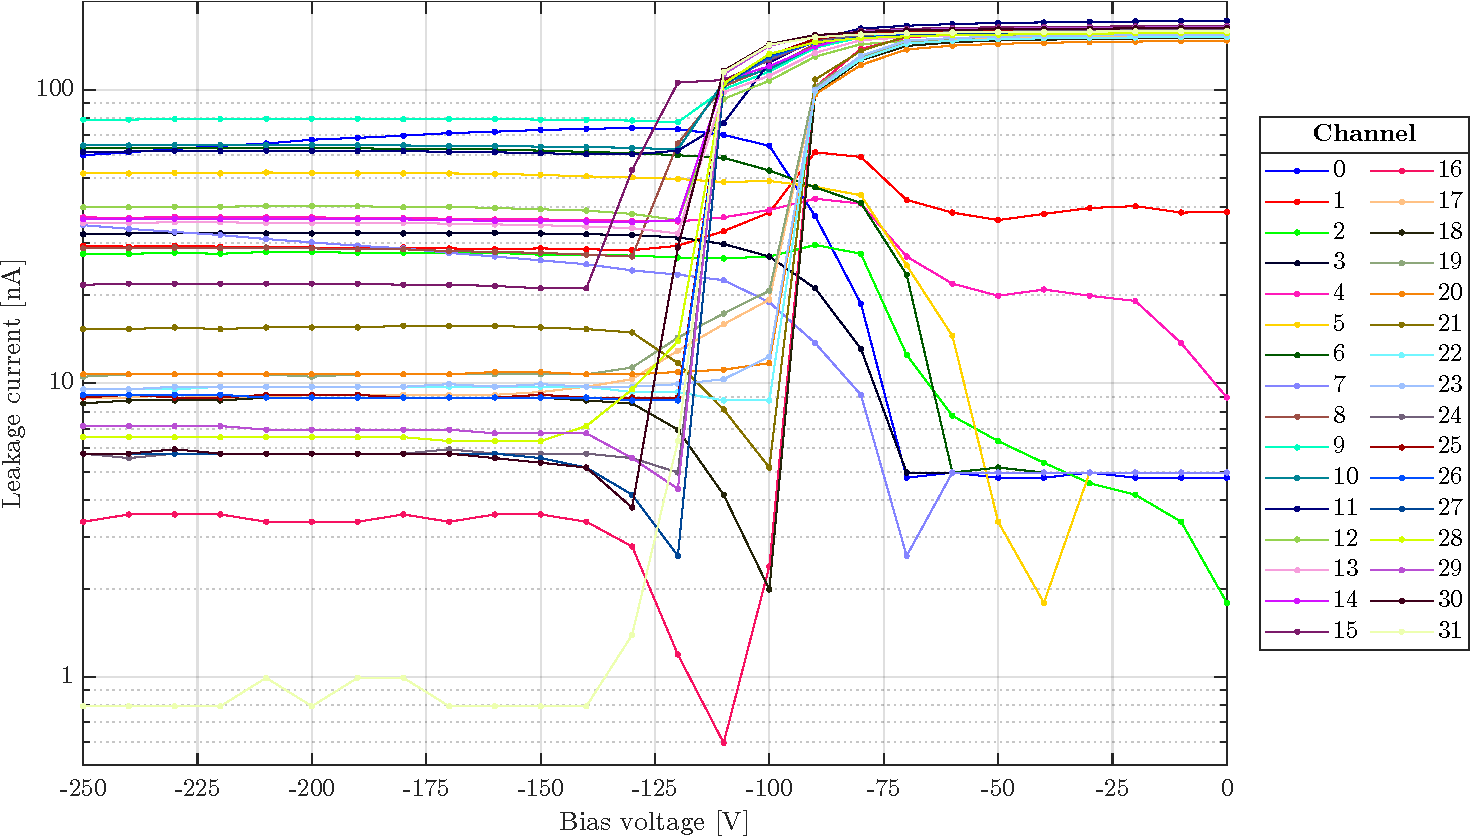
\includegraphics[width=1\textwidth]{images/backup_slides/leakage_current.pdf}
            \fontsize{8.5pt}{1}\selectfont
            \vspace{0.1cm}
            \begin{itemize}
                \item Si(Li) detector biased using a Caen HiVolta high voltage power supply
                \item Bias voltage comprised between \textbf{\SI{0}{\volt}} and \textbf{\SI{-250}{\volt}}
                \item Leakage current measured with ASIC internal circuit
                \item Measurement carried out at \textbf{\SI{-40}{\celsius}}
            \end{itemize}
            
        \column{0.4\textwidth}
            \centering
            \includegraphics[width=0.95\textwidth]{images/backup_slides/leakage_current_ch_250V.pdf}
            \fontsize{8.5pt}{1}\selectfont
            \vspace{0.1cm}
            \begin{itemize}
                \setlength\itemsep{0.7em}
                \item Measurement carried out with Si(Li) detectors biased at \textbf{\SI{-250}{\volt}}
                \item \textbf{\SI{71.13}{\nano\ampere}} maximum on channel 9
                \item \textbf{\SI{1.59}{\nano\ampere}} minimum on channel 31
                \item \textbf{\SI{746.11}{\nano\ampere}} in total over 32 channels is consistent with power supply readout
            \end{itemize}
        
    \end{columns}
    
\end{frame}

\backupend

\end{document}